\documentclass[11pt]{article}
\usepackage[T1]{fontenc}
\usepackage[utf8]{inputenc}
\usepackage{lmodern}
\usepackage[margin=1in]{geometry}
\usepackage{amsmath,amssymb,amsthm,mathtools,mathrsfs}
\usepackage{booktabs,enumitem,microtype}
\usepackage{placeins}
\usepackage{tikz}
\usetikzlibrary{arrows.meta,positioning,fit,calc,decorations.pathreplacing}
\usepackage[hidelinks]{hyperref}
\usepackage[capitalize,nameinlink,noabbrev]{cleveref}
\hypersetup{
  pdftitle={Harmonic heights and the Artin K(pi,1) conjecture},
  pdfauthor={OpenAI},
  pdfsubject={Contractibility of the full Artin Salvetti universal cover},
  pdfkeywords={Artin groups, Salvetti complex, Deligne complex, zigzag algebra, harmonic extension}
}
\newtheorem{theorem}{Theorem}[section]
\newtheorem{lemma}[theorem]{Lemma}
\newtheorem{proposition}[theorem]{Proposition}
\newtheorem{corollary}[theorem]{Corollary}
\theoremstyle{definition}
\newtheorem{definition}[theorem]{Definition}
\theoremstyle{remark}
\newtheorem{remark}[theorem]{Remark}
\numberwithin{equation}{section}
\newcommand{\C}{\mathbb C}
\newcommand{\R}{\mathbb R}
\newcommand{\Zbb}{\mathbb Z}
\DeclareMathOperator{\Hom}{Hom}
\DeclareMathOperator{\End}{End}
\DeclareMathOperator{\Cone}{Cone}
\DeclareMathOperator{\supp}{supp}
\DeclareMathOperator{\id}{id}
\DeclareMathOperator{\rad}{rad}
\setlist[enumerate]{itemsep=3pt,topsep=5pt}
\setlist[itemize]{itemsep=3pt,topsep=5pt}
\setlength{\emergencystretch}{1em}
\allowdisplaybreaks[1]
\title{Harmonic heights and the Artin \(K(\pi,1)\) conjecture}
\author{OpenAI}
\date{September 23, 2026}
\begin{document}
\maketitle
\begin{abstract}
We prove that the standard Salvetti complex of every Artin group with
finitely many standard generators is aspherical. This resolves the Artin
\(K(\pi,1)\) conjecture in finite rank.
\end{abstract}
\tableofcontents
\section{Introduction}\label{sec:introduction}

Let \(S\) be a finite set and \(M=(m_{st})_{s,t\in S}\) a Coxeter
matrix.  Thus \(m_{ss}=1\) and, for distinct \(s,t\), the symmetric
entry \(m_{st}\) belongs to
\(\{2,3,\ldots\}\cup\{\infty\}\).
The Artin group \(A=A(W,S)\) has generators \(\sigma_s\), with the
relation equating the two alternating words of length \(m_{st}\)
whenever \(m_{st}<\infty\).  The Coxeter group \(W\) is the quotient
obtained by imposing \(\sigma_s^2=1\).
A subset \(T\subseteq S\) is \emph{spherical} if its standard Coxeter
parabolic \(W_T\) is finite.

The standard Artin Salvetti complex \(X(W,S)\) has one cell of
dimension \(|T|\) for each spherical subset \(T\), including its
vertex for \(T=\varnothing\).  Its attaching maps come from the
oriented Coxeter-Salvetti construction.  These include the braid
relations in dimension two and the spherical cells in all higher
dimensions.  We recall the full model in
Section~\ref{sec:topology}.

\begin{theorem}\label{thm:main}
For every Coxeter matrix on a finite set \(S\), the universal cover
of \(X(W,S)\) is contractible.  Equivalently,
\[
  \pi_n\bigl(X(W,S)\bigr)=0\qquad(n\ge2).
\]
The conclusion allows arbitrary finite labels, infinite labels,
and connected or disconnected diagrams.
\end{theorem}

Thus Theorem~\ref{thm:main} resolves the \(K(\pi,1)\) conjecture
for Artin groups with finitely many standard generators.
The theorem concerns the full Salvetti complex: its
higher-dimensional cells are part of both the statement and the proof.
Although the generating set is finite, the Coxeter group need not be.

Theorem~\ref{thm:main} also supplies the asphericity input in several
established implications.  In Section~\ref{sec:consequences}, the
finite-dimensional classifying space gives torsion-freeness, and the
center theorem of Jankiewicz--Schreve~\cite[Theorem~3]{JankiewiczSchreve2022},
together with Deligne's spherical center theorem~\cite[Theorem~4.21]{Deligne1972},
gives \(Z(A)\cong\Zbb^k\), where \(k\) counts the connected
Coxeter-diagram components whose Coxeter groups are finite.  For the
positive Artin monoid, defined by the same generators and braid relations
in the category of monoids, Dobrinskaya's equivalence~\cite{Dobrinskaya2002},
as reproved by Ozornova~\cite[Section~5]{Ozornova2013}, gives the natural
equivalence of its classifying space with that of the group.  We also apply Boyd's
conditional stability theorem~\cite[Corollary~B]{Boyd2020} to its exact
family obtained by attaching a growing type-\(A\) path to a distinguished
vertex of an arbitrary fixed finite diagram, with no other new edges.
Its constant-coefficient range is recorded in
Corollary~\ref{cor:boyd-stability}.

\subsection{Context}

In spherical type, the geometric model is the complement of the
complexified reflection hyperplanes modulo the free action of the finite
Coxeter group.  Its fundamental group is the Artin group, and the
conjecture asks whether this orbit space is aspherical
\cite[Section~2]{Brieskorn1973}.  Modern accounts conventionally attribute
the origins of the conjecture to Arnol'd, Brieskorn, Pham and
Thom~\cite[Introduction]{Paolini2026}.
The Salvetti model connects the pairwise braid presentation with a
finite-dimensional cellular space governed by spherical parabolics.
Asphericity makes this explicit complex a classifying space, so its
cells and attaching maps encode group-topological invariants.

For ordinary braid groups, the configuration-space arguments of
Fadell--Neuwirth and Fox--Neuwirth give the basic example
\cite[Section~8]{FoxNeuwirth1962}.
Deligne proved the spherical case using finite real reflection
arrangements~\cite{Deligne1972}.  The positive-monoid structure in
finite type was developed by Brieskorn--Saito and
Deligne~\cite{BrieskornSaito1972,Deligne1972}.
Salvetti's cellular constructions give the relevant arrangement and
Coxeter models~\cite{Salvetti1987,Salvetti1994}; standard Artin
parabolics embed by van der Lek's
theorem~\cite{VanDerLek1983}.  Paolini gives a recent account of the
spherical theorem and its cell structure~\cite{Paolini2026}.

Charney--Davis developed the modified Deligne complex, built from
spherical parabolic cosets, and its equivalence to the asphericity
problem~\cite[Section~1.5 and Corollary~3.2.6]{CharneyDavis1995}.
They proved the FC case, in which every subset with all pairwise labels
finite is spherical, and the dimension-at-most-two case
\cite[Theorems~4.3.5--4.3.6 and Proposition~4.4.5]{CharneyDavis1995}.
Here dimension means the largest size of a spherical subset, which can
be much smaller than the rank $|S|$.
Paolini--Salvetti resolved all affine types using dual noncrossing
partitions and discrete Morse theory
\cite[Theorem~8.15]{PaoliniSalvetti2021}, building on the dual and
Garside constructions of McCammond--Sulway~\cite{McCammondSulway2017}.

Recent geometric methods cover further broad classes.
Huang--Przytycki proved the dimension-at-most-three case and additional
specified higher-dimensional classes
\cite[Theorems~1.1 and~12.20]{HuangPrzytycki2025}.
Hoda--Huang proved the conjecture when every irreducible spherical
parabolic is of type $A$, $B$, or $I_2$
\cite[Theorem~1.3]{HodaHuang2026}.
Huang's tree reduction~\cite[Theorem~1.1 and Corollary~9.2]{Huang2026}
requires both asphericity for tree diagrams and the condition that every
special four-cycle of alternating types in their Artin complexes has a
common neighboring vertex.  Our proof uses the classical spherical-coset reduction
and contracts that poset directly for every finite-rank matrix.

The algebraic tools have a different ancestry.  Zigzag algebras and
braid actions by evaluation cones were developed by
Huerfano--Khovanov, Khovanov--Seidel and Seidel--Thomas
\cite{HuerfanoKhovanov2001,KhovanovSeidel2002,SeidelThomas2001}.
Heng--Licata extend these constructions to fusion categories and
arbitrary Coxeter labels~\cite[Sections~4--5]{HengLicata2024}.
We use a framed version of that construction, with explicit choices of
fusion factors and edge objects.  The extreme-degree tests adapt the
positive-divisor method of Brav--Thomas for ADE configurations of
$2$-spherical objects~\cite[Section~3]{BravThomas2011}; here the tests
also apply to right simples and must recover original colors after
unfolding.  The proofs record these adaptations at their points of use.

Heng--Licata also relate their distinguished fusion-equivariant
stability component to Artin hyperplane complements and formulate its
contractibility as a route to the \(K(\pi,1)\) conjecture
\cite[Theorem~7.7 and Conjecture~7.12]{HengLicata2024}.  Here we contract
the spherical-coset poset directly.  The local requirements are a
two-point comparison of spherical cosets and an obstruction to an isolated
positive harmonic layer.  They combine categorical cohomology with
harmonic extension to control the links of a single well-ordered filtration.

\subsection{The proof and its local estimates}

Write \(\mathcal D\) for the poset of spherical right cosets
\(A_Tx\), ordered by inclusion with nested types.
The classical spherical theorem, the parabolic embedding theorem,
and Quillen's Theorem~A identify its order complex up to homotopy
with the full Salvetti universal cover
(Lemma~\ref{lem:salvetti-comparison}).
The task is therefore to contract \(|\mathcal D|\).
We add the vertices in a well-order.  A vertex's \emph{earlier link}
is the part of its link already present, and a \emph{source} has
empty earlier link.  If all earlier links are empty or contractible,
each component is contractible and has exactly one source
(Lemma~\ref{lem:filtration-principle}).  Thus controlling links and
distinguishing sources are the two topological tasks.

We adjoin a frame vertex and construct a finite graded zigzag
algebra.  An Artin element acts by invertible bimodule complexes.
Its action on the frame projectives has finitely many
\emph{layers}, indexed by the sum of cochain and internal
generator degrees.  Their nonnegative weighted multiplicities
give vectors \(m^d(x)\), with coordinates indexed by the original
colors \(S\) and the frame \(o\).  An original color means one
standard generator.  The frame coordinate is always one in layer
zero and zero in every other layer.
For distinct original colors $i,j\in S$, the diagram weights are
$b_{ij}=2\cos(\pi/m_{ij})$ for finite labels, $b_{ij}=2$ for
infinite labels, and $b_{io}=b_{oi}=1$ for frame edges.
For a spherical coset \(A_Tx\), the multiplicities outside \(T\) are
independent of the representative.  Their \emph{harmonic extension}
\(p=p^d(A_Tx)\) retains those exterior coordinates and solves
\[
 2p_i=\sum_{j\ne i}b_{ij}p_j\qquad(i\in T).
\]
Sphericity guarantees a unique nonnegative solution.
These vectors define the height: compare the highest nonnegative
layer first, and at each level resolve equality of vectors by a
type-order rule before comparing lower layers.

Passing to a larger spherical coset replaces more coordinates by
harmonic values; passing to a smaller coset exposes actual layer
multiplicities.  Positive-definite Cartan forms control strict
comparisons.  A different rule is needed when the harmonic vector at a
level \(q>0\) restricts on a connected component of its positive support
to a null vector for that component's Cartan matrix, and all higher
harmonic vectors vanish on the component and its boundary.  At those
components we reverse the type-order tie.  This rule permits the
upper-link contraction, but requires closed inequalities in certain
lower links.

Call data \emph{capped at \(q\)} on a set of colors if there are no
generators there above layer \(q\).  The lower-link problem leads to
two kinds of sublevel inside a fixed spherical coset \(A_Tx\) whose
boundary data are capped at \(q\).  For a proper subcoset
\(A_Jz\subsetneq A_Tx\), compare the exposed
counts \(m_i^q(z)\), \(i\in T\setminus J\), with the harmonic values
\(p_i^q(A_Tx)\), requiring these colors to be capped at \(q\).
Strict inequalities define the strict sublevel.  When \(T\) is contained
in a support component of this null kind, we also need the special
closed sublevel,
which permits equality.
Proposition~\ref{prop:residue-sublevels} proves that the strict
sublevel is empty or contractible, and that the special closed
sublevel is nonempty and contractible.  Its induction again uses
earlier links, so every component has a unique source.  The two
algebraic estimates supply source uniqueness and closed-sublevel
nonemptiness, respectively.

First, at a putative source \(A_Jz\), a lower bound valid at every
capped representative of that coset turns the excess above
\(p^q(A_Jz)\) into a convex combination of subrepresentation dimensions
(Proposition~\ref{prop:convex-subobjects}).
A three-step tensor filtration then compares two such sources.
The resulting two-point inequalities have a sum equal to the
negative of a positive-definite Cartan quadratic form, forcing
equality of their harmonic data.  Right-simple complexes supply
a parabolic detector that then identifies the actual cosets.
This proves uniqueness of the possible sources
(Proposition~\ref{prop:candidate-uniqueness}).

Second, emptiness of a special closed sublevel would mean that
every capped representative has all its interior counts strictly
above the prescribed null harmonic values.  The Hom calculation
in Section~\ref{sec:rigidity}, together with convexity, controls
a finite sequence of twists that simplifies successive lower
layers while retaining the cap.  It forces the boundary of the
null component to vanish in each layer reached by this process.
The fixed frame supplies a nonzero boundary coordinate in layer
zero, so the lowest nonzero boundary layer lies at or below zero.
Reaching that layer, below \(q>0\), gives a contradiction.  This is
the isolated harmonic-layer obstruction
(Proposition~\ref{prop:isolated-layer}).
The tensor and Hom arguments are proved independently of the
subsequent topological contraction.

With these residue sublevels available, the earlier upper and lower
links in the global filtration are empty or contractible.
The vertex-filtration principle makes each component contractible;
rank-one cosets connect all singleton cosets and hence the entire
poset.  This proves Theorem~\ref{thm:deligne-contractible}, and
the Salvetti comparison proves Theorem~\ref{thm:main}.

Figure~\ref{fig:dependencies} summarizes these dependencies.

\begin{figure}[tbp]
  \centering
  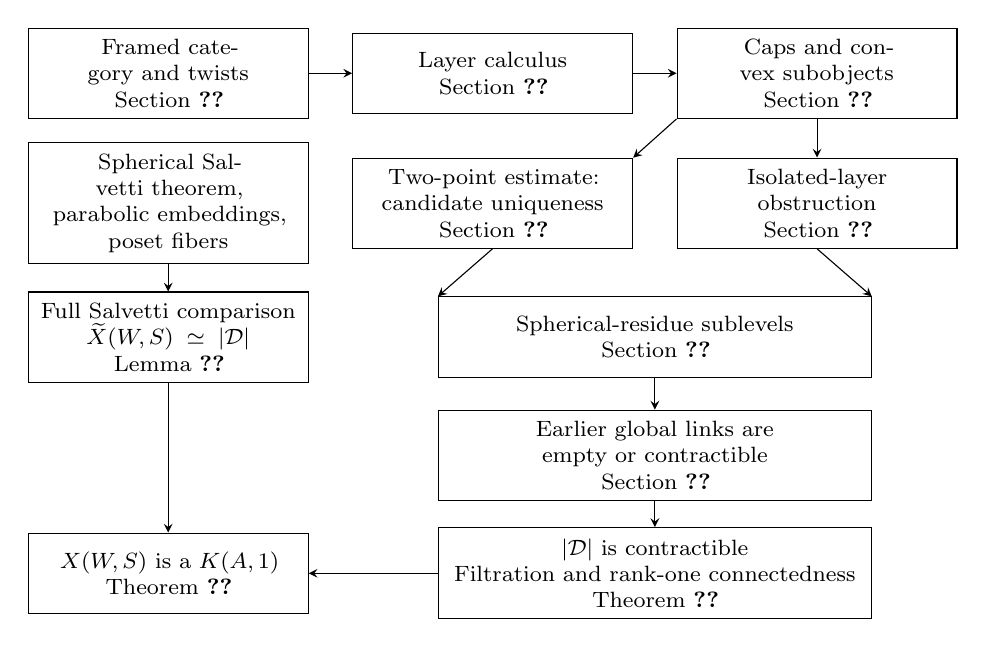
\begin{tikzpicture}[
      x=.01\linewidth,y=1cm,
      every node/.style={font=\footnotesize,align=center},
      result/.style={draw,thin,text width=.27\linewidth,
        minimum height=1.02cm,inner sep=4pt},
      wide/.style={result,text width=.43\linewidth},
      implication/.style={->,thin,>=stealth}
    ]
    \node[result] (category) at (0,0)
      {Framed category and twists\\Section~\ref{sec:category}};
    \node[result] (layers) at (34,0)
      {Layer calculus\\Section~\ref{sec:layers}};
    \node[result] (convexity) at (68,0)
      {Caps and convex subobjects\\Section~\ref{sec:height-data}};
    \node[result] (classical) at (0,-1.65)
      {Spherical Salvetti theorem,\\parabolic embeddings,\\poset fibers};
    \node[result] (two-point) at (34,-1.65)
      {Two-point estimate:\\candidate uniqueness\\Section~\ref{sec:two-point}};
    \node[result] (rigidity) at (68,-1.65)
      {Isolated-layer obstruction\\Section~\ref{sec:rigidity}};
    \node[result] (comparison) at (0,-3.35)
      {Full Salvetti comparison\\$\widetilde X(W,S)\simeq|\mathcal D|$\\
        Lemma~\ref{lem:salvetti-comparison}};
    \node[wide] (residues) at (51,-3.35)
      {Spherical-residue sublevels\\Section~\ref{sec:residues}};
    \node[wide] (links) at (51,-4.85)
      {Earlier global links are empty or contractible\\Section~\ref{sec:global}};
    \node[wide] (contractibility) at (51,-6.35)
      {$|\mathcal D|$ is contractible\\
        Filtration and rank-one connectedness\\
        Theorem~\ref{thm:deligne-contractible}};
    \node[result] (target) at (0,-6.35)
      {$X(W,S)$ is a $K(A,1)$\\Theorem~\ref{thm:main}};

    \draw[implication] (category) -- (layers);
    \draw[implication] (layers) -- (convexity);
    \draw[implication] (convexity.south west) -- (two-point.north east);
    \draw[implication] (convexity) -- (rigidity);
    \draw[implication] (two-point.south) -- (residues.north west);
    \draw[implication] (rigidity.south) -- (residues.north east);
    \draw[implication] (residues) -- (links);
    \draw[implication] (links) -- (contractibility);
    \draw[implication] (classical) -- (comparison);
    \draw[implication] (comparison) -- (target);
    \draw[implication] (contractibility) -- (target);
  \end{tikzpicture}
  \caption{The main dependencies.  The two algebraic estimates are proved
    before their use in the induction on spherical residues.  The classical
    comparison is independent of the height argument and transfers the
    resulting contraction to the full Salvetti universal cover.  Arrows
    display the main flow of the proof; the finite-type Coxeter and monoid
    inputs to the algebraic constructions are specified in the text.}
  \label{fig:dependencies}
\end{figure}


\subsection{Conventions and organization}

All posets are realized as their order complexes with the CW
topology.  All tensor categories and algebras are over \(\C\).
Complexes carry cochain and internal gradings; the total generator
degree is their sum.  Only cochain degrees determine differential
signs.  We use bimodule homotopy equivalences whenever a
nonprojective module will subsequently be tensored.
Subsets written with \(\subseteq\) need not be proper.

Section~\ref{sec:topology} fixes the topological model and the
classical inputs.
Sections~\ref{sec:category}--\ref{sec:height-data} construct the
algebra, its action, the layers and their convexity.
Sections~\ref{sec:two-point} and~\ref{sec:rigidity} prove the two
local estimates.
Sections~\ref{sec:residues} and~\ref{sec:global} establish the
sublevel theorem and the global contraction.
Section~\ref{sec:consequences} derives the structural consequences and
the homological-stability statement for fixed-core braid-tail families.

\section{The Salvetti complex and spherical parabolic cosets}
\label{sec:topology}

We first specify the space whose universal cover will be contracted.
Let $A=A(W,S)$ be the Artin group in Theorem~\ref{thm:main}, and let
\[
  \vartheta\colon A\longrightarrow W,
  \qquad \vartheta(\sigma_s)=s,
\]
be its Coxeter quotient.  For $T\subseteq S$, write $W_T=\langle T\rangle$
and $A_T=\langle\sigma_s:s\in T\rangle$, and put
\[
  \mathcal S^{\mathrm f}
  =\{T\subseteq S:W_T\text{ is finite}\}.
\]
The members of $\mathcal S^{\mathrm f}$ are called \emph{spherical}.
In particular, $\varnothing\in\mathcal S^{\mathrm f}$ and
$A_{\varnothing}=\{1\}$.

For a poset $\mathcal P$, its realization $|\mathcal P|$ will always mean
the order complex: vertices are elements of $\mathcal P$, simplices are
nonempty finite chains, and the realization has its CW topology.

\subsection{Classical inputs}

We use the following facts about Coxeter systems
\cite[Chapter IV, \S1, nos.~4--5 and 8]{Bourbaki2002}.
Each $(W_T,T)$ is the Coxeter
system defined by the submatrix on $T$.  A left coset of $W_R$ in
$W_T$, for $R\subseteq T$, has a unique element $u_0$ of minimal length,
and
\begin{equation}
  \ell(u_0v)=\ell(u_0)+\ell(v)
  \qquad(v\in W_R).
  \label{eq:topology-length-additivity}
\end{equation}
Reduced expressions for an element of $W$ are related by braid moves.
Consequently, if $w=s_1\cdots s_r$ is reduced, the element
\begin{equation}
  \iota(w)=\sigma_{s_1}\cdots\sigma_{s_r}\in A
  \label{eq:topology-positive-lift}
\end{equation}
is independent of the reduced expression.  Whenever
$\ell(uv)=\ell(u)+\ell(v)$, it satisfies
$\iota(uv)=\iota(u)\iota(v)$.

We also use the geometric representation and its chamber description:
the standard geometric form is positive definite exactly when the
Coxeter group is finite
\cite[Chapter V, \S4, no.~8, Theorem 2]{Bourbaki2002};
in finite type the chambers form a simply
transitive Coxeter orbit, signs of roots detect descents, and the
translates of a closed fundamental chamber cover the dual space
\cite[Chapter V, \S3, no.~3, and \S4, nos.~4 and 6]{Bourbaki2002}.
These assertions apply both to spherical submatrices of the original
system and to the finite Coxeter systems constructed below.

\begin{theorem}[Standard parabolic embedding]
\label{thm:topology-parabolic-embedding}
For every $T\subseteq S$, the homomorphism from the Artin group defined
by the submatrix on $T$ to $A$, sending its standard generators to the
corresponding $\sigma_t$, is injective.  Its image is $A_T$.
\end{theorem}

This is van der Lek's standard parabolic theorem
\cite[Chapter II, Section 4, Theorem 4.13(i)]{VanDerLek1983}.
No spherical hypothesis is imposed here.

The positive monoid on a subset $T$ means the monoid with the same
generators and positive braid relations as its Artin group.  Its
identity is the empty word.  An element $b$ \emph{right-divides} $a$
if $a=cb$ for some positive element $c$; left divisibility is defined
in the opposite order.

\begin{theorem}[Finite-type positive monoids]
\label{thm:topology-finite-monoid}
Suppose that $T$ is spherical, and let $A_T^+$ be its positive Artin
monoid.  Then the following statements hold.
\begin{enumerate}[label=\textup{(\roman*)}]
  \item The natural map $A_T^+\to A_T$ is injective.  In particular,
    $A_T^+$ is cancellative on both sides.
  \item Every element of $A_T$ can be written both as $ab^{-1}$ and
    as $c^{-1}d$, with $a,b,c,d\in A_T^+$.
  \item Any two elements of $A_T^+$ have a greatest common right
    divisor, and also a greatest common left divisor.
  \item If $w_T$ is the longest element of $W_T$, then
    $\Delta_T=\iota(w_T)$ is the finite-type fundamental element.
    Its left divisors and its right divisors coincide and are exactly
    the elements $\iota(w)$, $w\in W_T$.
\end{enumerate}
\end{theorem}

These are the finite-type monoid results of Brieskorn--Saito and
Deligne.  Cancellation and fractions are given in
\cite[Propositions 2.3 and 5.5(iii)--(iv), and Theorem 5.6]{BrieskornSaito1972} and
\cite[Theorem 4.14]{Deligne1972}; the gcd statement is
\cite[Proposition 4.2]{BrieskornSaito1972}.  For the fundamental
element and its divisors, see
\cite[Lemma 5.4 and Propositions 5.5 and 5.7]{BrieskornSaito1972}.
We use Theorem~\ref{thm:topology-finite-monoid} only for spherical
subsets and for finite Coxeter unfoldings.  In particular, fractions
in a positive monoid are never assumed for the full system when it
is not spherical.

\subsection{Permutahedral cells and their face maps}

For each nonempty spherical $T$, take a point in the interior of a
fundamental chamber of the finite reflection representation of $W_T$.
Choose these points compatibly with diagram components: on a reducible
system use the direct sum of the points chosen for its components.
The convex hull of its $W_T$-orbit is a Coxeter permutahedron $\Pi_T$.
It is a closed ball of dimension $|T|$, with vertices labeled by
$W_T$ and with a distinguished \emph{source} labeled $1$.
Set $\Pi_{\varnothing}$ to be a point.

The nonempty faces of $\Pi_T$ are indexed by cosets $u_0W_R$, where
$R\subseteq T$ and $u_0$ is the shortest element of its coset.
The face with this index will be denoted $F_{u_0,R}$; its vertices
have labels $u_0v$, $v\in W_R$.  There is a specified cellular
homeomorphism
\begin{equation}
  j_{u_0,R}\colon \Pi_R\longrightarrow F_{u_0,R},
  \qquad v\longmapsto u_0v
  \quad\text{on vertices}.
  \label{eq:topology-face-identification}
\end{equation}
One precise choice is obtained by taking the barycentric subdivisions
of both face lattices, sending the center of the face $v_0W_Q$ to the
center of $u_0v_0W_Q$, and extending affinely over their simplices.
Centers on product faces are chosen as products of the centers of
their factors.

These identifications are compatible on nested faces.  Indeed, if
$v_0$ is the shortest representative of a left $W_Q$-coset in $W_R$,
then \eqref{eq:topology-length-additivity} makes $u_0v_0$ the shortest
representative of the corresponding left $W_Q$-coset in $W_T$.
On barycentric subdivisions this gives the equality
\begin{equation}
  j_{u_0,R}\circ j_{v_0,Q}=j_{u_0v_0,Q}.
  \label{eq:topology-nested-faces}
\end{equation}

Define $X(W,S)$ by taking one copy of $\Pi_T$ for every
$T\in\mathcal S^{\mathrm f}$ and, for every proper face
$F_{u_0,R}\subset\Pi_T$, identifying $j_{u_0,R}(y)$ with the point
$y$ in the copy of $\Pi_R$.  Equation~\eqref{eq:topology-nested-faces}
makes all these identifications compatible.  The resulting CW complex
has one open $|T|$-cell of each spherical type $T$.

An edge in a model cell whose endpoints are $u_0$ and $u_0s$, with
$\ell(u_0s)=\ell(u_0)+1$, projects to the edge of type $s$, oriented
positively.  This convention fixes the attaching maps, including their
orientations.  Equivalently, the Coxeter Salvetti complex has cells
$(w,T)$, $w\in W$, $T\in\mathcal S^{\mathrm f}$, with the same models
and face parameters $(wu_0,R)$.  Its $W$-action is left multiplication
on $w$, and its quotient has precisely the identifications just given.
Thus this is the oriented Coxeter--Salvetti model
\cite[Theorem~1.4]{Salvetti1994}; compare
\cite[Theorem~3.3 and Section~5]{Paolini2026}.

The one-skeleton has one vertex and one oriented edge $\sigma_s$ for
each $s\in S$.  If $\{s,t\}$ is spherical, its model is a $2m_{st}$-gon.
The two increasing paths from its source to its opposite vertex read
the two alternating words of length $m_{st}$.  Its attaching relation
is their equality.  If $m_{st}=\infty$, there is no cell of this type.
It follows that the two-skeleton is the Artin presentation complex,
and hence
\begin{equation}
  \pi_1(X(W,S))=A.
  \label{eq:topology-fundamental-group}
\end{equation}
The cells of dimension at least three remain part of $X(W,S)$.

We invoke the spherical theorem in the following precise form.

\begin{theorem}[Spherical asphericity]
\label{thm:topology-spherical-asphericity}
If $T$ is spherical, the universal cover of the CW complex
$X(W_T,T)$ with the preceding permutahedral attaching maps is
contractible.
\end{theorem}

Deligne proved asphericity of the corresponding finite reflection
arrangement complement \cite[opening theorem, p.~273]{Deligne1972}.
The Salvetti formulation is given, for example, in
\cite[Theorem 3.3 and Corollary 5.7]{Paolini2026}.
The hypothesis here is finiteness of $W_T$, not merely finiteness
of its generating set.

\subsection{The regular universal cover}

Let $\widetilde X$ be the universal cover of $X(W,S)$, and label its
vertices by $A$, with the vertex $1$ chosen over the unique vertex of
$X(W,S)$.  A positive edge of type $s$ goes from $\alpha$ to
$\alpha\sigma_s$.  A lift of a cell of type $T$ is uniquely determined
by the lift $\alpha$ of its source, so denote this open cell by
$(\alpha,T)$.

A reduced gallery from the source of $\Pi_T$ to its vertex $u$ reads
a reduced word for $u$.  Its lift therefore ends at $\alpha\iota(u)$.
In particular, the face indexed by $u_0W_R$ has parameter
\begin{equation}
  (\alpha\iota(u_0),R),
  \qquad R\subseteq T,
  \quad u_0\text{ shortest in }u_0W_R\subseteq W_T.
  \label{eq:topology-lifted-faces}
\end{equation}
The corresponding characteristic map on that face is
\eqref{eq:topology-face-identification}.  Compatibility also follows
directly from
$\iota(u_0v_0)=\iota(u_0)\iota(v_0)$.

The lifted CW structure is regular.  To see this, consider two open
faces of a single $\Pi_T$.  If their types differ, their lifted cells
differ.  If both have type $R$, with shortest representatives $u_0$
and $u_1$, equality of their lifted parameters would give
$\alpha\iota(u_0)=\alpha\iota(u_1)$.  Applying $\vartheta$ gives
$u_0=u_1$, so the faces coincide.  Each open face maps
homeomorphically to its lifted cell.  It follows inductively on
dimension that the characteristic map of $\Pi_T$ is injective on its
whole closed ball.  Since the model is compact and the cover is
Hausdorff, this map is an embedding.  Thus the face poset
$\mathcal F(\widetilde X)$ has realization canonically homeomorphic
to the barycentric subdivision of $\widetilde X$.

\subsection{The spherical-coset comparison}

The modified Deligne complex of Charney--Davis is built from spherical
parabolic cosets~\cite[Section~1.5]{CharneyDavis1995}.  We use its
right-coset presentation.  Define
\begin{equation}
  \mathcal D
  =\{A_Tx:x\in A,\ T\in\mathcal S^{\mathrm f}\},
  \label{eq:topology-deligne-poset}
\end{equation}
with types retained, ordered by coset inclusion with nested types.
Thus $A_Ry\le A_Tx$ means $R\subseteq T$ and
$A_Ry\subseteq A_Tx$.  Inversion identifies this poset with the
left-coset poset
$\mathcal D^{\ell}=\{xA_T:x\in A,\ T\in\mathcal S^{\mathrm f}\}$.

We use the following form of Quillen's Theorem A
\cite[Section 1, Theorem A and its dual formulation]{Quillen1973}:
if $f\colon\mathcal P\to\mathcal Q$ is a map of small posets and
\[
  \bigl|f^{-1}(\mathcal Q_{\le q})\bigr|
  \quad\text{is contractible for every }q\in\mathcal Q,
\]
then $|f|\colon|\mathcal P|\to|\mathcal Q|$ is a homotopy equivalence.
Here $\mathcal Q_{\le q}=\{q'\in\mathcal Q:q'\le q\}$ is the whole
lower ideal, and the posets and fibers need not be finite.

\begin{lemma}[Salvetti--coset comparison]
\label{lem:salvetti-comparison}
There is a homotopy equivalence
\[
  \widetilde X(W,S)\simeq|\mathcal D|.
\]
Consequently, contractibility of $|\mathcal D|$ implies the conclusion
of Theorem~\ref{thm:main}.
\end{lemma}

\begin{proof}
Define
\[
  f\colon\mathcal F(\widetilde X)\longrightarrow\mathcal D^{\ell},
  \qquad f(\alpha,T)=\alpha A_T.
\]
Formula~\eqref{eq:topology-lifted-faces} makes $f$ order preserving:
if $(\alpha\iota(u_0),R)$ is a face of $(\alpha,T)$, then
$\iota(u_0)\in A_T$ and $R\subseteq T$, so
$\alpha\iota(u_0)A_R\subseteq\alpha A_T$.

Fix $\beta A_T\in\mathcal D^{\ell}$.  The inverse image of its
lower ideal consists exactly of the cells
\begin{equation}
  (\alpha,R),\qquad \alpha\in\beta A_T,\quad R\subseteq T.
  \label{eq:topology-fiber-cells}
\end{equation}
Indeed, the indicated conditions imply
$\alpha A_R\subseteq\beta A_T$, and the converse follows from the
retained types and from $\alpha\in\alpha A_R$.

By Theorem~\ref{thm:topology-parabolic-embedding}, write
$\alpha=\beta h$ uniquely with $h$ an element of the Artin group on
$T$.  Under this correspondence, every face formula becomes
\[
  (h,R)\longmapsto(h\iota(u_0),Q),
  \qquad Q\subseteq R\subseteq T,
\]
with $u_0$ the shortest representative of the specified $W_Q$-coset
in $W_R$.  These are exactly the lifted face maps of $X(W_T,T)$.
Thus the poset in \eqref{eq:topology-fiber-cells} is its universal-cover
face poset.  Its realization is contractible by
Theorem~\ref{thm:topology-spherical-asphericity}.  For $T=\varnothing$
it is a single vertex.

Quillen's Theorem A now gives
$|\mathcal F(\widetilde X)|\simeq|\mathcal D^{\ell}|$.
Regularity identifies the left side with a subdivision of
$\widetilde X$, and inversion identifies the right side with
$|\mathcal D|$.  This proves the lemma.
\end{proof}

\begin{remark}
The comparison uses the full spherical universal covers over lower
ideals, including all their higher cells.  It does not assert that the
translation action on $\mathcal D$ is free: its vertex stabilizers are
conjugates of standard parabolic subgroups.  The classical comparison appears in
\cite[Corollary~3.2.6]{CharneyDavis1995}; it is also established in the
more general framework of
\cite[Section 3, Theorem 3.1 and Lemma 3.2]{GodelleParis2012}.
\end{remark}

We record two elementary coset facts for the later link calculations.
If $R\subseteq T$ and $A_Ry$ meets $A_Tx$, then
$A_Ry\subseteq A_Tx$.  For a fixed coset $A_Ry$ and a specified
larger spherical type $T$, its unique upper extension is $A_Ty$.
Thus lower intervals can be computed entirely inside the indicated
parabolic subgroup, and upper extensions are determined by their
types.  These assertions use only inclusions with nested types.

Finally, if $T=T_1\sqcup\cdots\sqcup T_r$ is the decomposition into
components of its Coxeter diagram, the presentation and
Theorem~\ref{thm:topology-parabolic-embedding} give
\begin{equation}
  A_T=A_{T_1}\times\cdots\times A_{T_r}.
  \label{eq:topology-parabolic-product}
\end{equation}
Cosets of subgroups whose types lie in these blocks, and their
inclusion relations, are accordingly products.  When $S$ is empty,
both $X(W,S)$ and $|\mathcal D|$ are points; in the rest of the proof
we may assume $S\ne\varnothing$.

\section{A framed category and its Artin action}
\label{sec:category}

We construct a finite graded algebra and a homotopy action of the Artin
group on complexes of its projectives. The construction uses a fusion
category to realize the nonintegral entries of the geometric Coxeter
form.  This is a framed variant of the fusion-category zigzag construction
and Artin action of Heng--Licata~\cite[Sections~4--5]{HengLicata2024}.
We use a full Temperley--Lieb factor for each edge with finite label
at least four, its string
object as edge label, and an additional frame.  These choices differ
from their default labels; compare their Remarks~4.4 and~5.4.
We give the algebra and its bimodule homotopies for these conventions.

\subsection{The geometric form and a frame}

Adjoin a vertex $o$, called the frame, to the original finite set $S$,
and put $\widehat S=S\sqcup\{o\}$. For distinct original vertices set
\[
 b_{ij}=\begin{cases}
 2\cos(\pi/m_{ij}),&m_{ij}<\infty,\\
 2,&m_{ij}=\infty,
 \end{cases}
 \qquad b_{io}=b_{oi}=1\quad(i\in S).
\]
Let $C$ be the symmetric matrix indexed by $\widehat S$ with diagonal
entries $2$ and off-diagonal entries $-b_{ij}$. An edge means a pair with
$b_{ij}>0$; in particular a label $2$ gives no edge. The frame is not an
Artin generator. If $T\subseteq\widehat S$, write $C_T$ for the
corresponding principal submatrix, and write $\partial T$ for the vertices
outside $T$ adjacent to a vertex of $T$. This boundary includes the frame
when appropriate.

We use the standard geometric representation of Coxeter systems: on
root-coefficient vectors the simple reflection at $i$ is
\begin{equation}
 s_i p=p-(Cp)_i\varepsilon_i,
 \label{eq:category-reflection}
\end{equation}
where $\varepsilon_i$ is the $i$th coordinate vector. Its restriction to
the coordinates of a parabolic subsystem is its geometric
representation. The standard Coxeter theorems identify spherical
$T\subseteq S$ with the positive definite matrices $C_T$
\cite[Chapter~V, \S4, no.~8, Theorem~2]{Bourbaki2002}. We also use
the root-sign criterion for descents and the fact that reduced
expressions are related by braid moves; these are Coxeter-system
theorems, without a finiteness assumption on the ambient system
\cite[Chapter~IV, \S1; Chapter~V, \S4, nos.~4 and~6]{Bourbaki2002}.
Whenever the chamber covering or a
longest element is used below, the subsystem concerned has first been
shown to be finite.

\begin{lemma}
\label{lem:cartan-positive-null}
For a spherical subset $T\subseteq S$, the inverse $C_T^{-1}$ is
entrywise nonnegative, and is strictly positive within each connected
diagonal block. Prescribing the coordinates of $p$ outside $T$ therefore
determines a unique vector harmonic on $T$, by which we mean
$(Cp)|_T=0$. Nonnegative prescribed coordinates give a nonnegative
harmonic extension.

More generally, let $G$ be a nonempty connected vertex set. If
$v_i>0$ for $i\in G$ and $C_Gv\geq0$ coordinatewise, then either
$C_G$ is positive definite or $C_Gv=0$.
\end{lemma}

\begin{proof}
Write $C_T=2I-B_T$, where $B_T$ is symmetric and entrywise nonnegative.
Positive definiteness implies that the largest eigenvalue of $B_T$ is
less than $2$. The Perron--Frobenius bound for a nonnegative symmetric
matrix then gives spectral radius less than $2$, so
\[
 C_T^{-1}=\frac12\sum_{n\geq0}(B_T/2)^n.
\]
This is nonnegative, and a path between any two vertices in the same
block gives a strictly positive entry in some power. Harmonic extension
is explicitly
\[
 p_T=C_T^{-1}B_{T,\widehat S\setminus T}
                 p_{\widehat S\setminus T},
\]
which proves the first assertions, including uniqueness.

For the last assertion, every real vector $x$ on $G$ satisfies
\begin{equation}
 x^{\mathsf t}C_Gx
 =\sum_{\substack{i<j\\i,j\in G}}b_{ij}v_iv_j
       \left(\frac{x_i}{v_i}-\frac{x_j}{v_j}\right)^2
   +\sum_{i\in G}\frac{(C_Gv)_i}{v_i}x_i^2.
 \label{eq:category-scaled-form}
\end{equation}
If at least one coordinate of $C_Gv$ is positive, vanishing of this
quadratic form forces all $x_i/v_i$ to be equal by connectedness, and
then forces their common value to be zero. The form is therefore
positive definite. If none is positive, the assumed inequalities say
exactly that $C_Gv=0$.
\end{proof}

\subsection{Fusion labels}

The ingredients are the Jones--Wenzl projectors and the spherical
quotient by negligible maps.  We recall their construction to fix the
normalization; see Wenzl~\cite{Wenzl1987},
Barrett--Westbury~\cite[Theorem~2.9]{BarrettWestbury1999}, and the
Temperley--Lieb account in Chen~\cite[Sections~5.1--5.4]{Chen2014}.
The finite semisimplicity below uses the specific projector decomposition,
in addition to the general spherical quotient construction.

\begin{proposition}
\label{prop:fusion-construction}
There is a finite semisimple spherical $\C$-linear tensor category
$\mathscr C$ with strictly positive real dimensions, and, for every
ordered edge $(s,t)$ of $\widehat S$, an object $D^1_{st}$ of dimension
$b_{st}$, with $D^1_{ts}$ its dual, having the following properties.
For every finite edge and simple objects $L,L'$,
\[
 \dim_\C\Hom_{\mathscr C}(L,D^1_{st}\otimes L')\leq1.
\]
On a label-$3$ edge or a frame edge one may take $D^1_{st}=\mathbf1$;
on an infinite edge one may take $D^1_{st}=\mathbf1\oplus\mathbf1$.
\end{proposition}

\begin{proof}
For each individual finite edge of label $m\geq4$, use an independent
Temperley--Lieb factor with circle value
\[
 d_m=2\cos(\pi/m),\qquad
 [j]=\frac{\sin(j\pi/m)}{\sin(\pi/m)}.
\]
Here is its construction. Begin with the pivotal diagram category whose
objects are nonnegative tensor powers of a self-dual string and whose
morphisms are $\C$-linear combinations of planar pairings. Composition
is stacking, a closed circle is replaced by $d_m$, and tensor product
is juxtaposition. Closing a diagram gives its spherical trace. Take the
additive idempotent completion, quotient by the ideal of negligible
maps, and complete additively and idempotently again. A map $f:X\to Y$
is negligible if $\operatorname{tr}(gf)=0$ for every $g:Y\to X$.
Cyclicity proves stability under composition, and partial trace proves
stability under tensoring; hence this is a tensor ideal.

For completeness, the idempotents and decompositions in this quotient
can be obtained directly. Let $f_0$ and $f_1$ be the respective identity
diagrams, and define, for $1\leq j\leq m-2$,
\begin{equation}
 f_{j+1}=p-\frac{[j]}{[j+1]}p e_jp,
 \qquad p=f_j\otimes\id,
 \label{eq:category-jw-recursion}
\end{equation}
where $e_j$ is the unnormalized cap--cup at the last two positions.
All denominators in this recursion are nonzero. Inductively $f_j$ is
idempotent, kills every elementary turnback on either side, and its
partial trace over the last string is
\begin{equation}
 \operatorname{ptr}(f_j)=\frac{[j+1]}{[j]}f_{j-1}
 \qquad(1\leq j\leq m-1).
 \label{eq:category-jw-partial-trace}
\end{equation}
Indeed the partial trace of the two terms defining $f_j$ is
$d_m f_{j-1}-([j-1]/[j])f_{j-1}^2$, which is the right side of
\eqref{eq:category-jw-partial-trace}; the case $j=1$ starts the
induction. Sandwiched between the last cap--cups, $p$ consequently gives
$([j+1]/[j])(f_{j-1}\otimes e)$, where $e$ is the last cap--cup.
Since $p$ already factors through $f_{j-1}$ on the first $j-1$ strings,
this identity shows that the subtracted term in
\eqref{eq:category-jw-recursion} is a projection, proves idempotence
of $f_{j+1}$, and proves its turnback cancellation. The last cap and cup
factor that projection through $f_{j-1}$; their opposite composite is
the nonzero scalar $[j+1]/[j]$. Thus its image is isomorphic to
$f_{j-1}$, giving
\begin{equation}
 f_j\otimes f_1\cong f_{j+1}\oplus f_{j-1}
 \qquad(1\leq j<m-1).
 \label{eq:category-string-fusion}
\end{equation}
Closing \eqref{eq:category-jw-partial-trace} gives
$\operatorname{tr}(f_j)=[j+1]$.

A planar pairing between the corners of $f_i$ and $f_j$ has a turnback
unless $i=j$ and it is the straight pairing. Consequently these corners
vanish for $i\ne j$ and are one-dimensional for $i=j$. The object
$f_{m-1}$, whose trace is $[m]=0$, is therefore negligible. The objects
$f_0,\ldots,f_{m-2}$ survive, are simple, and have positive dimensions
$[1],\ldots,[m-1]$. The decompositions
\eqref{eq:category-string-fusion}, with $f_{m-1}$ now zero, generate
every tensor power from these objects. Thus the quotient is finite
semisimple. Reflecting the diagrams gives the same fusion rule on the
other side: the turnback-killing idempotent with straight coefficient
one is unique, as follows by multiplying any two such idempotents.
Duality and the spherical trace descend to the quotient and its
completions. This proves all the stated properties of a single factor.

Take the tensor product of these finitely many categories, with simple
objects the tuples of simple objects in the factors and tensor product
and Hom spaces given factorwise. If there are no such factors, take
finite-dimensional vector spaces. For an edge of label $m\geq4$, use
the string object $f_1$ in its factor and units in the other factors.
Tensoring by it has the path-$A_{m-1}$ multiplicities in that factor and
fixes the others, proving the multiplicity bound. The choices of units
and two units cover the remaining edges. All dimensions are products
of positive dimensions. Choose dual objects for opposite orientations
and use the opposite pivotal evaluations on the two orientations.
\end{proof}

Fix representatives $\operatorname{Irr}(\mathscr C)$ of the simple
objects, and put
\[
 w_L=\dim_{\mathscr C}L>0
 \qquad(L\in\operatorname{Irr}(\mathscr C)).
\]
The tensor category is not required to be symmetric. In what follows
the labels are always tensored on the right, and evaluation of an edge
and its dual occurs on the left of those labels.

\subsection{The graded algebra and its pairing}

Ordinary zigzag algebras and their graded-symmetric pairing are developed
by Huerfano--Khovanov~\cite[Section~3, Proposition~1]{HuerfanoKhovanov2001}.
The following projective category is the basic-algebra realization of
the fusion-labelled version; compare
\cite[Section~4.4, Proposition~4.13]{HengLicata2024}.

For $s\in\widehat S$ and $X\in\mathscr C$ introduce an additive
projective symbol $P_{s,X}$. Besides $D^1_{st}$ on edges, set
$D^0_{ss}=D^2_{ss}=\mathbf1$ and set every unspecified $D^a_{st}$ to
zero. Define the length-$a$ morphisms by
\begin{equation}
 \Hom^a(P_{s,X},P_{t,Y})
   =\Hom_{\mathscr C}(X,D^a_{st}\otimes Y).
 \label{eq:category-projective-hom}
\end{equation}
The length-zero units act as identities. For two length-one maps,
composition is obtained by first tensoring their label maps and then
applying
\[
 D^1_{st}\otimes D^1_{ts}\longrightarrow\mathbf1=D^2_{ss}
\]
on a backtrack. All other products of two positive lengths are zero.
For opposite directions use the left and right pivotal evaluations.
This is associative: the assertion involving a length-zero map is
functoriality, and both products of any three positive lengths are
zero.

An unfolded vertex is a pair $\alpha=(s,L)$ with $L$ simple. For a set
of colors $T$ write $\widetilde T=T\times\operatorname{Irr}(\mathscr C)$.
Let $Z$ be the finite-dimensional basic graded algebra with
\begin{equation}
 e_\alpha Z e_\beta=\Hom(P_\alpha,P_\beta),
 \label{eq:category-path-order}
\end{equation}
where multiplication is in path order. With this convention
$P_\alpha=Ze_\alpha$ is a left projective and
$\Hom_Z(Ze_\alpha,Ze_\beta)=e_\alpha Ze_\beta$ as required. Put
$Q_\alpha=e_\alpha Z$ for the right projective.
Let $U_\alpha$ be the simple top of $Q_\alpha$, concentrated in
cochain and internal degrees zero. Decomposing $X$ into
simples expresses $P_{s,X}$ as a sum of the $P_\alpha$'s. The algebra
has only lengths $0,1,2$; length zero is the semisimple diagonal, and
length two is one-dimensional on each unfolded diagonal. Write
$t_\alpha$ for the length-two token corresponding to $\id_L$ when
$\alpha=(s,L)$.

\begin{lemma}
\label{lem:category-frobenius}
The functional $\tau:Z\to\C$ defined by
\[
 \tau(t_{s,L})=w_L,
 \qquad \tau(Z^0\oplus Z^1)=0
\]
is a symmetric Frobenius trace of degree $-2$. Thus
$\theta_\alpha=t_\alpha/w_L$ has trace one. The radical of $Z$ is
$Z^{>0}$, and the socle of each indecomposable left or right projective
is its token subspace.

For every finite graded bimodule $M$, the adjoint dual has a natural
bimodule identification
\begin{equation}
 M^\vee:=\Hom_{Z\text{-left}}(M,Z)
       \cong D_\C(M)\langle2\rangle,
 \label{eq:category-adjoint-duality}
\end{equation}
where $D_\C$ is graded vector-space duality and $\langle a\rangle$
raises degrees by $a$. It is an involutive contravariant equivalence,
fixes the regular bimodule, and satisfies
\begin{equation}
 (P_\alpha\otimes_\C Q_\beta)^\vee
       \cong(P_\beta\otimes_\C Q_\alpha)\langle-2\rangle.
 \label{eq:category-projective-dual}
\end{equation}
In particular this duality preserves additive radicals.
\end{lemma}

\begin{proof}
The length-zero and length-two spaces pair perfectly. For length one,
duality identifies maps $L'\to D^1_{ts}\otimes L$ with maps
$D^1_{st}\otimes L'\to L$. Pairing these against
$L\to D^1_{st}\otimes L'$ by the semisimple trace is nondegenerate:
on every simple summand the ordinary matrix trace is multiplied by its
nonzero categorical dimension. This is exactly the backtrack pairing.
Its symmetry is the pivotal partial-trace identity. Namely, the trace
on $L$ of the first backtrack equals the trace on
$D^1_{st}\otimes L'$ of the opposite composite; taking partial trace
in $D^1_{st}$ gives the second pivotal cap and then the trace on $L'$.
Hence $\tau(ab)=\tau(ba)$. This is ordinary symmetry; it has no sign
from internal degree.

The positive-length ideal is nilpotent and the quotient is the
semisimple diagonal, so it is the radical. Tokens are annihilated by
this radical. A nonzero length-one element has a nonzero product with
a suitable opposite arrow by the perfect pairing, and a nonzero
length-zero element has a nonzero product with its token. Therefore
the token is the entire socle of each projective.

For \eqref{eq:category-adjoint-duality}, send $f$ to $\tau\circ f$.
A homogeneous $f$ of degree $k$ gives a functional of degree $k-2$,
which explains the shift $\langle2\rangle$. Nondegeneracy of the trace
gives the usual Frobenius identification for every finite left module.
It respects both bimodule actions: with
$(a f b)(m)=f(ma)b$ one has
\[
 \tau(f(ma)b)=\tau(bf(ma))=\tau(f(bma)),
\]
which is the action $(a\lambda b)(m)=\lambda(bma)$ on the vector dual.
The shifted vector dual squares naturally to the identity, so this is
a contravariant equivalence. Such an equivalence preserves the
additive radical, characterized by invertibility of $1-gf$ for all
opposite maps $g$.

The trace identifies
$D_\C(P_\alpha)=Q_\alpha\langle-2\rangle$ and
$D_\C(Q_\beta)=P_\beta\langle-2\rangle$. Vector duality reverses
the factors of an external tensor product; combining its shift $-4$
with the shift $+2$ in \eqref{eq:category-adjoint-duality} proves
\eqref{eq:category-projective-dual}. The same trace identifies
$D_\C(Z)\langle2\rangle$ with $Z$.
\end{proof}

\subsection{Finite Coxeter unfoldings}

Fusion unfolding replaces labelled vertices by their simple constituents;
see Heng--Licata~\cite[Section~8]{HengLicata2024}.
For the chosen factors we prove the positivity and descent properties
that will be needed for finite-type braid and termination arguments.

Define a symmetric matrix $\widetilde C$, indexed by unfolded vertices,
with diagonal $2$ and off-diagonal entries
\[
 \widetilde C_{\alpha\beta}
       =-\dim_\C(e_\alpha Z^1e_\beta).
\]
Symmetry follows also from the perfect edge pairing. Define
\begin{equation}
 (\phi p)_{s,L}=w_Lp_s.
 \label{eq:category-phi}
\end{equation}
Fusion and duality imply
\begin{equation}
 \widetilde C\phi p=\phi Cp.
 \label{eq:category-intertwining}
\end{equation}
Indeed, for fixed $L$ and an edge object $D$, the weighted sum of
$\dim\Hom_{\mathscr C}(L,D\otimes L')$ over $L'$ is
$\dim(D)w_L$: adjunction identifies these multiplicities with those
of $L'$ in $D^*\otimes L$, whose dimension is $\dim(D)w_L$.
Equation~\eqref{eq:category-intertwining} also holds on any color
submatrix.

We write $D_L(w)=\{s:\ell(sw)<\ell(w)\}$ and
$D_R(w)=\{s:\ell(ws)<\ell(w)\}$ for the left and right descent sets,
where $s$ ranges over the simple generators of the Coxeter system
in question.

\begin{lemma}
\label{lem:finite-unfolding}
If $J\subseteq S$ is spherical, then $\widetilde C_{\widetilde J}$
is positive definite and simply laced, and defines a finite Coxeter
system. Replacing each original letter $s_i$, $i\in J$, by the product
of the commuting reflections in all vertices of its color gives a
lift of words to this system. For every such word representing $w$,
its lifted product $\widetilde w$ has
\begin{equation}
 D_L(\widetilde w)=\widetilde{D_L(w)},\qquad
 D_R(\widetilde w)=\widetilde{D_R(w)}.
 \label{eq:category-descents}
\end{equation}
Reduced expressions lift to reduced expressions, and a reduced
expression for the longest element of $W_J$ lifts to a reduced
expression for the longest element of the unfolded system.
\end{lemma}

\begin{proof}
The positive vector
$v=\phi(C_J^{-1}\mathbf1)$ satisfies
$\widetilde C_{\widetilde J}v=\phi\mathbf1>0$.
Applying the scaled quadratic-form identity
\eqref{eq:category-scaled-form} to each connected component proves
positive definiteness of the entire unfolded matrix. In particular
this proves positivity on directions outside the image of $\phi$.
An infinite edge cannot lie in $J$, since its two-by-two Cartan matrix
is singular. The multiplicity assertion of
Proposition~\ref{prop:fusion-construction} therefore makes every
off-diagonal unfolded entry either $0$ or $-1$. The finite Coxeter
criterion applies.

There are no edges between different vertices of a single color.
Their reflections commute, and
\eqref{eq:category-intertwining} shows that their product on a folded
vector is the original reflection
\eqref{eq:category-reflection}. Choose $p$ with $C_Jp>0$. Then
$\phi p$ lies in the interior of a full unfolded fundamental chamber,
since every row of $\widetilde C_{\widetilde J}\phi p$ is positive.
For any word, intertwining identifies its image with $\phi(wp)$.
The row at an unfolded vertex $\alpha$ on this image tests the sign
of $\widetilde w^{-1}\alpha$, while the corresponding original row
tests the sign of $w^{-1}\alpha_i$.

To see why this is a complete sign test, a root of either finite
system has either all nonnegative or all nonpositive coefficients in
the simple-root basis. Pairing it with one chamber-interior point is
therefore strictly positive or strictly negative respectively. No
assumption about the dimension of the folded subspace or about its
orbit meeting every unfolded chamber is needed. The intertwining
identity multiplies the original row by $w_L>0$, proving the equality
of left descent sets. Applying the same argument to reversed words
proves the equality of right descent sets. The lifted product depends
only on the original group element as well: a word for the identity
fixes $\phi p$, and the stabilizer of a chamber-interior point in the
finite unfolded reflection group is trivial
\cite[Chapter~V, \S3, no.~3]{Bourbaki2002}.

Suppose an original reduced expression is extended by an ascent
letter. Every vertex of its color is an ascent of the lifted prefix
by \eqref{eq:category-descents}. After one reflection of that color,
the others remain ascents, because they are orthogonal to it.
Consequently the whole block is a sequence of successive ascents.
Induction proves reducedness of the lift. Finally the longest
original element has every original simple reflection as a descent.
Its lift has every unfolded simple reflection as a descent, and hence
is the longest unfolded element.
\end{proof}

\subsection{Twist bimodules}

Two-term evaluation bimodules are the standard algebraic model for
spherical twists.  The inverse calculations below follow the method of
Khovanov--Seidel~\cite[Section~2d, Proposition~2.4]{KhovanovSeidel2002};
for fusion-labelled zigzags see
\cite[Definition~5.2, Proposition~5.3]{HengLicata2024}.

All complexes are bounded cochain complexes of finite internally
graded modules or bimodules. Differentials have cochain degree one and
internal degree zero. The internal shift $\langle a\rangle$ raises
degrees by $a$, while $[1]$ lowers cochain placements by one. Tensor
products and Hom complexes use the ordinary cochain signs only; the
internal grading contributes no additional signs. Graded Hom retains
both degrees.

Put $M_\alpha=P_\alpha\otimes_\C Q_\alpha$. Multiplication gives
$\mu_\alpha:M_\alpha\to Z$. The perfect trace pairing between
$P_\alpha$ and $Q_\alpha$ gives the central tensor
\[
 \delta_\alpha(1)=\sum_a p_a\otimes q_a,
 \qquad \tau(q_ap_b)=\delta_{ab},
\]
where the bases are homogeneous. It has internal degree two, and
invariance of the pairing proves its centrality, so it defines a
bimodule map $Z\to M_\alpha\langle-2\rangle$. Define
\begin{equation}
 B_\alpha=[M_\alpha\xrightarrow{\mu_\alpha} Z],
 \qquad
 D_\alpha=[Z\xrightarrow{\delta_\alpha}
                   M_\alpha\langle-2\rangle],
 \label{eq:category-twists}
\end{equation}
with $Z$ in cochain degree zero in both complexes. Thus the projective
terms of $B_\alpha,D_\alpha$ lie in degrees $-1,1$, respectively.

\begin{lemma}
\label{lem:category-twist-inverse}
There are bigraded bimodule chain homotopy equivalences
\[
 B_\alpha\otimes_ZD_\alpha\simeq Z
       \simeq D_\alpha\otimes_ZB_\alpha.
\]
\end{lemma}

\begin{proof}
The product has terms $M_\alpha$ in degree $-1$,
\[
 Z\oplus
 P_\alpha\otimes_\C(e_\alpha Ze_\alpha)
                 \otimes_\C Q_\alpha\langle-2\rangle
\]
in degree zero, and $M_\alpha\langle-2\rangle$ in degree one.
Split the middle factor as
$e_\alpha Ze_\alpha=\C e_\alpha\oplus\C\theta_\alpha$.
The incoming differential projects isomorphically, up to its cochain
sign, onto the token summand. Explicitly, the token coefficient of
$q p_a$ is $\tau(q p_a)$, and the identity
$\sum_a\tau(qp_a)q_a=q$ is the dual-basis identity. Cancel this
degree-$-1$/degree-zero isomorphism. The outgoing differential from
the remaining unit summand is the identity onto
$M_\alpha\langle-2\rangle$, by multiplication with $e_\alpha$;
cancel it as well. The remaining complex is the regular bimodule $Z$
in degree zero. These are Gaussian cancellations of actual bimodule
complexes. In the reverse tensor order the dual-basis identity and
unit multiplication give the same two cancellations, with the
opposite tensor order and the prescribed cochain signs.
\end{proof}

We record the spherical-twist conjugation argument used for braid
relations, following Seidel--Thomas~\cite[Lemma~2.11 and
Propositions~2.12--2.13]{SeidelThomas2001} with the required bimodule
homotopies. For a
bounded perfect left complex $P$, define its evaluation twist to be
the bimodule cone
\begin{equation}
 T_P=\Cone\bigl(P\otimes_\C\Hom_Z(P,Z)\longrightarrow Z\bigr).
 \label{eq:category-evaluation-twist}
\end{equation}
It is unchanged up to homotopy by either shift of $P$. It is also
unchanged under a homotopy equivalence of $P$: a chosen homotopy
inverse and its homotopies identify the two evaluation morphisms up
to homotopy and identify their cones. If $B$ is an invertible
bimodule complex of the kind generated by
\eqref{eq:category-twists}, then
\begin{equation}
 B\otimes_ZT_P\otimes_ZB^{-1}\simeq T_{B\otimes_ZP}.
 \label{eq:category-conjugation}
\end{equation}
Here all terms of $B$ are finite projective on each side: they are
sums of shifts of $Z$ and of $P_\alpha\otimes_\C Q_\beta$.
The left-module dual $B^\vee=\Hom_Z(B,Z)$, with the usual complex
signs, is its tensor adjoint. The evaluation and coevaluation for
finite projectives give the adjunction identities at chain level.
Invertibility therefore identifies $B^\vee$ with $B^{-1}$ in the
bimodule homotopy category. Lemma~\ref{lem:category-frobenius} shows
that these duals remain in the same class of terms. Tensor--Hom
identifies the dual of $B\otimes_ZP$ with
$\Hom_Z(P,Z)\otimes_ZB^\vee$, and under this identification the
composed evaluations agree. Taking their cones proves
\eqref{eq:category-conjugation}.

\begin{lemma}
\label{lem:category-local-braid}
If there is no arrow between distinct unfolded vertices $\alpha,\beta$,
then $B_\alpha B_\beta\simeq B_\beta B_\alpha$. If there is exactly
one arrow in each direction, then
\[
 B_\alpha B_\beta B_\alpha
       \simeq B_\beta B_\alpha B_\beta.
\]
Products here and below denote tensor products over $Z$.
\end{lemma}

\begin{proof}
In the first case $M_\alpha M_\beta=0=M_\beta M_\alpha$, so both
products are the simultaneous evaluation cone with projective term
$M_\alpha\oplus M_\beta$.

In the second case, $B_\alpha P_\beta$ has the nonzero arrow
$P_\alpha\langle1\rangle\to P_\beta$ in degrees $-1,0$.
The complex $D_\beta P_\alpha$ has the nonzero arrow
$P_\alpha\to P_\beta\langle-1\rangle$ in degrees $0,1$.
Nondegeneracy of the edge pairing makes both arrows nonzero, and
their common Hom space is one-dimensional. Therefore
\[
 B_\alpha P_\beta\simeq
       (D_\beta P_\alpha)\langle1\rangle[1],
\]
after rescaling one term if needed. Their evaluation twists agree.
Since $T_{P_\gamma}=B_\gamma$, conjugation gives
\[
 B_\alpha B_\beta D_\alpha
       \simeq D_\beta B_\alpha B_\beta.
\]
Multiplying on the left by $B_\beta$ and on the right by $B_\alpha$
gives the claimed braid relation.
\end{proof}

\begin{proposition}
\label{prop:twist-action}
For each original color $i$, let
\[
 B_i=\prod_{\alpha\in\widetilde{\{i\}}}B_\alpha,
 \qquad
 D_i=\prod_{\alpha\in\widetilde{\{i\}}}D_\alpha.
\]
These products are independent of their order up to bimodule homotopy.
The assignments $\sigma_i\mapsto B_i$ and $\sigma_i^{-1}\mapsto D_i$
define an action of the original Artin group by invertible bimodule
homotopy classes. For $x\in A$ write $B_x$ for a representing complex,
and write $F_i=B_i\otimes_Z-$ on left complexes.

For every $H\in\mathscr C$, right tensoring of labels,
\[
 T_H(P_{s,X})=P_{s,X\otimes H},
\]
is an additive functor on projectives that preserves path lengths and
extends to their bounded homotopy category. It commutes naturally up
to homotopy with the positive and inverse color twists, and hence
with each $B_x\otimes_Z-$. All the action identities above are
bimodule chain homotopy equivalences, so they remain valid upon
tensoring with finite complexes of modules that are not projective.
\end{proposition}

\begin{proof}
Distinct vertices in a color have no mutual Hom spaces. Their twists
commute by Lemma~\ref{lem:category-local-braid}, and their products
are inverse by Lemma~\ref{lem:category-twist-inverse}. Moreover
\begin{equation}
 B_i\cong
 \Cone\left(\bigoplus_{\alpha\in\widetilde{\{i\}}}
               P_\alpha\otimes_\C Q_\alpha\longrightarrow Z\right):
 \label{eq:category-color-cone}
\end{equation}
every mixed tensor term in the expansion vanishes by orthogonality.

If $m_{ij}<\infty$, the subsystem on $\{i,j\}$ is spherical.
The two alternating words of length $m_{ij}$ are reduced expressions
for its longest element. By Lemma~\ref{lem:finite-unfolding}, both
lift to reduced expressions for the same longest element of its
finite simply-laced unfolding. Matsumoto's theorem relates these
expressions by commutations and three-term braid moves, all of which
hold for the bimodules by Lemma~\ref{lem:category-local-braid}.
This proves the original Artin relation. When $m_{ij}=\infty$ there
is no relation to verify. Thus the assignment defines the asserted
homotopy action for every Coxeter matrix under consideration.

On a morphism in \eqref{eq:category-projective-hom}, $T_H$ is
right tensoring by $\id_H$, with the associativity identifications.
All cap multiplications are to the left of the label, so this
preserves composition and path length. In the evaluation term of
\eqref{eq:category-color-cone} applied to $P_{t,Y}$, semisimplicity
gives the canonical identification
\begin{align*}
 &\bigoplus_{a,L}
    P_{i,L}\langle a\rangle\otimes_\C
      \Hom_{\mathscr C}(L,D^a_{it}\otimes Y)\\
 &\hspace{35mm}\cong
      \bigoplus_a P_{i,D^a_{it}\otimes Y}\langle a\rangle.
\end{align*}
Its evaluation is the tautological label map. Tensoring this
description on the right by $H$ is the same description with $Y$
replaced by $Y\otimes H$, naturally in $Y$ and its projective
morphisms. Hence the evaluation cones commute naturally with $T_H$
on projectives and on their complexes. Whiskering this natural
commutation by the inverse equivalence proves the same assertion
for $D_i$, without requiring $T_H$ itself to be invertible.

Finally, tensoring an explicit chain homotopy and its equations with
any module complex preserves those equations with the ordinary
cochain tensor signs. The last assertion therefore follows from
the homotopy-level inverse and braid calculations, without any
flatness requirement on these additional module complexes.
\end{proof}

We will extract the height data from the images $B_xP_{o,L}$ of the
frame projectives, for $x\in A$ and all simple labels $L$.  Retaining
the whole label family will allow us to combine its generator counts,
using the positive label dimensions, into vectors indexed by the
original colors and the frame.  We first need to extract these counts
from homotopy classes.  The next section uses minimal complexes and
groups their generators into layers according to $c+u$, where $c$ is
the cochain placement and $u$ is the internal generator degree.

\section{Layers and cohomological tests}
\label{sec:layers}

We turn the twist action into a calculus of generator layers.  The
objectives are to detect the top and socle of a layer by ordinary
cohomology and to bound the layers created by a reduced spherical word.
These bounds will make the later cap-preserving operations possible.

We work in the homotopy category of bounded complexes of finite graded
left projective $Z$-modules.  A differential has cochain degree $1$ and
internal degree $0$.  The internal shift $\langle u\rangle$ raises
internal degrees by $u$, whereas $[1]$ lowers cochain placements by one.
Thus a generator of a copy of $P_\alpha\langle u\rangle$ in cochain
degree $c$ has \emph{level}
\begin{equation}
 d=c+u.
 \label{eq:layers-level}
\end{equation}
Generator dimensions always count copies of projectives, rather than
the vector-space dimensions of the projectives themselves.

\subsection{Minimal complexes and the linear heart}

A bounded projective complex is \emph{minimal} if each differential
entry belongs to the graded radical of the additive category of
projectives.  Any invertible entry between shifted indecomposables can
be removed by Gaussian elimination, splitting off a contractible
two-term complex.  There are finitely many summands, so this procedure
ends in a minimal complex.  Such a model is unique up to chain
isomorphism: a homotopy equivalence between two minimal complexes is
termwise invertible modulo the additive radical, since the homotopies
are composed with radical differentials.  Each term map is therefore
invertible, by the Krull--Schmidt property of finite graded module
terms.  This also proves the corresponding minimality statement for
any of the finite additive categories of module or bimodule terms
used below.

In a minimal complex a nonzero differential entry has path length
$a=1$ or $2$.  Its generator placements change by $(1,-a)$, and hence
its level changes by $1-a$.  The entries of length one preserve the
level, and those of length two lower it by one.  For a minimal complex
$E$, let $Y^d(E)$ be the complex consisting of the generators of level
$d$, with the length-one part of the differential.  This is a complex:
the length-two component of the equation $\partial^2=0$ is exactly
the square of its length-one part.

More concretely, write $V^d_{\alpha,c}(E)$ for the multiplicity space
of $P_\alpha\langle d-c\rangle$ in cochain degree $c$.  A coefficient
of a length-one differential is a map
\[
 V^d_{\alpha,c}(E)\longrightarrow V^d_{\beta,c+1}(E)
\]
for a chosen functional on $e_\alpha Z^1e_\beta$.  These coefficient
maps satisfy the backtrack relation obtained by multiplying opposite
arrows in $Z^2$.  There are no other length-two products to impose.
All these arrays are finite, and every coefficient arrow raises $c$.
In particular their paths act nilpotently.

At an unfolded vertex $\alpha$, the \emph{top} of such an array is
the generator space modulo the images of all incoming coefficient
maps, and its \emph{socle} is the common kernel of all outgoing
coefficient maps.  These spaces retain their cochain and internal
placements.  We write $\operatorname{top}_\alpha M$ and
$\operatorname{soc}_\alpha M$ for them, and write
$\dim M_\alpha$ for the sum of the generator multiplicities over
all placements at $\alpha$.

\begin{lemma}[Layer structure]\label{lem:layer-structure}
The full subcategories defined by minimal generator levels $d\leq0$
and $d\geq0$ form a bounded $t$-structure.  Its truncation
$\tau_{\leq k}E$ is represented by the subcomplex of a minimal model
on levels at most $k$; the complementary quotient represents
$\tau_{\geq k+1}E$.

The heart is equivalent to the abelian category of finite graded
coefficient arrays just described.  In particular, subobjects of a
pure layer, after shifting that layer into the heart, are precisely
graded subrepresentations of its array.  The unshifted cohomology
layer at $d$ is $Y^d(E)$.
\end{lemma}

\begin{proof}
The level calculation shows that the indicated low terms form a
subcomplex, with the indicated high quotient.  An internal- and
cochain-degree-zero map from a generator of level $d$ to one of
level $e$ would require a path of length $d-e$.  Consequently every
such map from levels at most $0$ to levels at least $1$ is zero.
This gives the required orthogonality.  The cochain shift $[1]$
decreases all levels by one, giving the two shift-closure axioms.
The short exact sequence of low subcomplex, full complex, and high
quotient gives the truncation triangle.  There are finitely many
occupied levels, so the $t$-structure is bounded.

Between pure objects of the same level, a degree-zero map has only
length-zero entries.  It is therefore exactly a graded map of their
multiplicity arrays commuting with the coefficient arrows.  A
cochain homotopy would have cochain degree $-1$ and would require
path length $-1$, so there are no homotopies to quotient out.
Conversely every finite array satisfying the backtrack relation
defines a pure complex of projectives.  Kernels and cokernels of
array maps, taken in each graded coefficient space, still satisfy
the relation.  This identifies the heart with the asserted abelian
category.  Applying the truncations twice identifies its cohomology
layers with the complexes $Y^d(E)$.
\end{proof}

We use the usual long exact cohomology sequence of a $t$-structure
\cite[Theorem~1.3.6]{BBD1982}.  To distinguish it from the vector-space tests
below, denote the heart-valued cohomology by $H^d_{\mathrm{lay}}$;
our conventions give
\[
 H^d_{\mathrm{lay}}(E)=Y^d(E)[d],\qquad
 H^d_{\mathrm{lay}}(E[1])=H^{d+1}_{\mathrm{lay}}(E).
\]
The corresponding fusion-category linear-heart construction appears in
\cite[\S6.1]{HengLicata2024}.

An exact functor has \emph{layer amplitude} $[a,b]$ if it sends each
pure layer at $d$ to levels in $[d+a,d+b]$.  By bounded truncations,
the same statement gives the corresponding bounds on an arbitrary
interval of input levels.

\begin{lemma}[Adjacent-layer exact sequences]
\label{lem:layers-amplitude-extension}
Suppose that an exact functor $F$ has layer amplitude $[0,1]$.
For any $E$ and any $d$, there is a short exact sequence
\begin{equation}
\begin{split}
0\longrightarrow Y^d\bigl(F(Y^{d-1}(E))\bigr)
\longrightarrow Y^d(FE)
\longrightarrow Y^d\bigl(F(Y^d(E))\bigr)
\longrightarrow0,
\end{split}
\label{eq:layers-adjacent-positive}
\end{equation}
where all terms are shifted by $[d]$ when regarded as objects of the
heart.  In particular their generator dimensions are additive.

For amplitude $[-1,0]$, the corresponding sequence is
\begin{equation}
0\longrightarrow Y^d\bigl(F(Y^d(E))\bigr)
\longrightarrow Y^d(FE)
\longrightarrow Y^d\bigl(F(Y^{d+1}(E))\bigr)
\longrightarrow0.
\label{eq:layers-adjacent-negative}
\end{equation}
\end{lemma}

\begin{proof}
In the positive case apply $F$ to
\[
 \tau_{\leq d-1}E\longrightarrow\tau_{\leq d}E
 \longrightarrow Y^d(E).
\]
The first term has levels at most $d$, and the last term has levels
$d,d+1$.  The flanking groups in the long exact sequence at $d$ are
$H^{d-1}_{\mathrm{lay}}F(Y^d(E))$ and
$H^{d+1}_{\mathrm{lay}}F(\tau_{\leq d-1}E)$; both are zero.
This gives a short exact sequence at that level.  Applying $F$ to
the truncation below $d-1$ identifies its left term with the one in
\eqref{eq:layers-adjacent-positive}, since levels at most $d-2$ map
to levels at most $d-1$.  Applying it to the truncation above $d$
identifies the middle term with $Y^d(FE)$, since levels at least
$d+1$ remain at least $d+1$.

For the negative case use
$\tau_{\leq d}E\to\tau_{\leq d+1}E\to Y^{d+1}(E)$.
After $F$ the first term has levels at most $d$, and the last has
levels $d,d+1$.  The same exact-sequence argument, now discarding
input levels below $d$ and above $d+1$, gives
\eqref{eq:layers-adjacent-negative}.
\end{proof}

\begin{lemma}[Composition at the bottom]
\label{lem:layers-bottom-composition}
Suppose that each of $F_1,\ldots,F_r$ is exact and has no negative
change of layer level.  Starting from a pure layer at $d$, the
level-$d$ part of $F_r\cdots F_1$ is obtained by retaining only the
level-$d$ part after each intermediate operation.  In particular,
any relation between such composed functors gives the corresponding
relation between their operations on the bottom layer.
\end{lemma}

\begin{proof}
After the first operation the quotient by its level-$d$ truncation
has levels at least $d+1$.  Every subsequent functor keeps that
quotient in levels at least $d+1$.  The long exact sequence therefore
identifies bottom cohomology before and after discarding it.
Repeat this argument at each step.
\end{proof}

\subsection{Extremal tests and single twists}

When vector-space cohomology retains both gradings, we write
$H^t(V)$ for the direct sum of its cohomology spaces whose cochain
degree plus internal degree is $t$.  Differentials raise this total
degree by one.  Only cochain degrees enter the signs.

\begin{lemma}[Extremal cohomological tests]
\label{lem:layers-extremal-tests}
For a pure layer $M$ at level $d$,
\begin{equation}
 H^d(e_\alpha M)\cong\operatorname{soc}_\alpha M,
 \qquad
 H^{d+2}(e_\alpha M)\cong
                  (\operatorname{top}_\alpha M)\langle2\rangle,
 \label{eq:layers-extremal-tests}
\end{equation}
as graded multiplicity spaces, with their corresponding placements.
The shift on the top is the internal placement of the token.
If a minimal complex $E$ has no generators above $d$ at $\alpha$
or its neighbors, its test in degree $d+2$ is still
$(\operatorname{top}_\alpha Y^d(E))\langle2\rangle$, and all
higher test cohomology there vanishes.
If it has no generators below $d$ at those vertices, its test in
degree $d$ is the socle of $Y^d(E)$ at $\alpha$.

A nonzero pure layer supported on a vertex set has a nonzero top
and a nonzero socle somewhere in that set.
\end{lemma}

\begin{proof}
For a pure layer at $d$, the paths in $e_\alpha M$ have lengths
$0,1,2$, and their total degrees are respectively $d,d+1,d+2$.
At the length-zero end, being a cycle means being killed by every
outgoing coefficient map.  At the token end, the incoming maps span
exactly the images of the incoming coefficient maps, because the
opposite-arrow pairing is nondegenerate.  This proves
\eqref{eq:layers-extremal-tests}.

For the upper assertion, every term of $e_\alpha E$ comes from a
generator at $\alpha$ or a neighbor.  Its actual total degree is its
generator level plus its path length, and is therefore at most
$d+2$.  At degree $d+2$ only the level-$d$ token terms occur.
Their incoming differential consists of the indicated linear maps:
any additional contribution would need a higher generator at the
same vertex or a neighbor.  The lower assertion follows in the same
way from the length-zero end.  Finally, the coefficient arrows
strictly raise cochain placement in a finite array.  Iterating them
cannot avoid a socle, and iterating incoming images cannot generate
a nonzero array with zero top everywhere.
\end{proof}

Let $F_i=B_{\sigma_i}(-)$ be the positive color twist from
Proposition~\ref{prop:twist-action}.  Write $r_i$ for the product of
the commuting coordinate reflections in its unfolded fiber.  On
vectors of generator multiplicities this changes only that fiber.

\begin{lemma}[Positive layers]\label{lem:positive-layer}
Each $F_i$ has layer amplitude $[0,1]$.  Its upper piece on a pure
layer $M$ at $d$ is supported on the fiber of $i$, has no arrows,
and has multiplicity $\dim\operatorname{top}_\alpha M$ at a vertex
$\alpha$ of that fiber.  Its bottom piece has unchanged
multiplicities at all other vertices, and at $\alpha$ in the fiber
it has multiplicity
\begin{equation}
 \dim Y^d(F_iM)_\alpha
 =\sum_\beta(2\id-\widetilde C)_{\alpha\beta}
       \dim M_\beta
       -\dim M_\alpha+\dim\operatorname{top}_\alpha M.
 \label{eq:layers-positive-dimension}
\end{equation}
The bottom piece has zero socle in color $i$.  If $M$ has zero
socle in every color of a set $J$ containing $i$, its bottom piece
after $F_i$ also has zero socle in all of $J$.

For any bounded left complex $E$, without a projectivity assumption
on its terms, there is a natural homotopy equivalence of test
complexes
\begin{equation}
 e_\alpha F_iE\simeq(e_\alpha E)\langle2\rangle[1]
 \qquad(\alpha\text{ of color }i).
 \label{eq:layers-positive-test-shift}
\end{equation}
There is the identical statement for right complexes tested on the
right.
\end{lemma}

\begin{proof}
For pure input at $d$, the simultaneous evaluation cone inserts
generators in color $i$ at levels $d+a-1$, for path lengths
$a=0,1,2$.  Those at $d-1$ are the length-zero evaluation copies.
Their maps to the old generators of color $i$ are identities modulo
the additive radical.  Cancelling these pairs removes all
generators below $d$.  None were inserted above $d+1$, proving the
amplitude bound.  Only the acted color can occur above $d$.

For one vertex $\alpha$ of this color put $A=e_\alpha E$.
All other vertices of the same color are orthogonal to it, so its
simultaneous test is
\begin{equation}
 \Cone\bigl(A\oplus A\langle2\rangle
       \xrightarrow{(\id,\theta_\alpha)}A\bigr).
 \label{eq:layers-token-cone}
\end{equation}
Projection onto the token source summand
$A\langle2\rangle[1]$ is a chain map with kernel the cone of
$\id_A$.  It is therefore a homotopy equivalence, proving
\eqref{eq:layers-positive-test-shift} for arbitrary input.
The same calculation works on the right.  For pure input, the
degree-$d+3$ test on the output is the old degree-$d+2$ test.
Lemma~\ref{lem:layers-extremal-tests} identifies it with the upper
generator multiplicities and with the old top, respectively.
There are no arrows among the vertices of the upper piece.

For completeness, signed generator counts are computed with
$(-1)^d$.  A contractible scalar pair has consecutive levels, so
its two signed contributions cancel.  In the cone for one vertex,
the inserted signed contribution from a generator at $\beta$ is
minus the alternating path count
$2\delta_{\alpha\beta}-(2\id-\widetilde C)_{\alpha\beta}$.
Thus the total signed vector transforms by $r_i$.  Since the
output has only levels $d,d+1$, subtracting its upper vector from
its bottom vector gives $r_i\dim M$.  The upper vector is the old
top.  At the acted fiber this gives
\eqref{eq:layers-positive-dimension}; outside it the multiplicities
are unchanged.

At a vertex of color $i$, the degree-$d$ test of $F_iM$ is zero
by \eqref{eq:layers-positive-test-shift}, so its bottom socle is
zero.  For a vertex $\beta$ of another color the evaluation
triangle for $e_\beta F_iM$ has first term a sum of copies of
$(e_\alpha M)\langle1\rangle$, with $\alpha$ in the acted fiber
adjacent to $\beta$.  Its cohomology at $d$ is zero, and its
cohomology at $d+1$ is a sum of the old socles at those $\alpha$.
If the socles in $J$ vanish, the long exact sequence at $d$,
together with the old socle vanishing at $\beta$, gives the
claimed vanishing at $\beta$ after the move.
\end{proof}

\begin{lemma}[Inverse amplitude]\label{lem:layers-inverse-amplitude}
If an exact equivalence $F$ has layer amplitude $[0,1]$, its inverse
has amplitude $[-1,0]$.  In particular each $F_i^{-1}$ has that
amplitude and satisfies
\begin{equation}
 e_\alpha F_i^{-1}E\simeq
       (e_\alpha E)\langle-2\rangle[-1]
 \qquad(\alpha\text{ of color }i),
 \label{eq:layers-negative-test-shift}
\end{equation}
with the analogous formula for right complexes.

For either sign, acting in color $i$ leaves the generator
multiplicities in every layer unchanged at all other colors.
\end{lemma}

\begin{proof}
It suffices to test the inverse on a heart object $X$.  If $A$ has
levels at most $-2$, then $FA$ has levels at most $-1$, whence
\[
 \Hom(A,F^{-1}X)=\Hom(FA,X)=0.
\]
Orthogonality implies that $F^{-1}X$ has levels at least $-1$.
If $B$ has levels at least $1$, then $FB$ does also, and
\[
 \Hom(F^{-1}X,B)=\Hom(X,FB)=0.
\]
It follows that $F^{-1}X$ has levels at most $0$.  This proves the
inverse bound; shifting proves it for every pure level.
Formula~\eqref{eq:layers-negative-test-shift} follows by applying
\eqref{eq:layers-positive-test-shift} to $F_i^{-1}E$ and using
invertibility.  This argument is at the homotopy level also for
nonprojective test inputs.

For $\beta$ outside the acted color, the right simple $U_\beta$
satisfies
\[
 U_\beta B_{\sigma_i}^{\pm1}\simeq U_\beta,
\]
because all the inserted projective bimodule terms have left
vertex in color $i$.  Tensoring a minimal left projective complex
with $U_\beta$ kills its radical differential and counts precisely
its generators at $\beta$, with both placements retained.  The
displayed identity therefore proves the last assertion in every
layer.
\end{proof}

\subsection{Positive divisors detected by cohomology}

Fix a spherical subset $J$.  Its unfolding is a finite simply-laced
Coxeter system by Lemma~\ref{lem:finite-unfolding}.  In the next two
lemmas the letters are its individual unfolded vertices.  For a
bounded left complex $X$ put
\begin{equation}
 h_J(X)=\max\{t:H^t(e_\alpha X)\ne0
                        \text{ for some }\alpha\in\widetilde J\},
 \label{eq:layers-test-height}
\end{equation}
and set $h_J(X)=-\infty$ if all these tests vanish.  For right
complexes replace $e_\alpha X$ by $Xe_\alpha$.  The statements
require only bounded test cohomology; the input need not be a
projective complex.

The next two lemmas use the extreme-degree method of
Brav--Thomas~\cite[Lemma~3.3 and Proposition~3.1]{BravThomas2011}.
They work with finite ADE configurations of $2$-spherical objects.
We give the total-degree calculation on both module sides, including
the nonprojective right simples needed below, and then pass from
unfolded vertices to the original colors.

\begin{lemma}[Change of test height]\label{lem:layers-height-change}
For a positive unfolded letter $\alpha$, if $h_J(X)$ is finite,
\[
 h_J(X)\leq h_J(B_\alpha X)\leq h_J(X)+1.
\]
An increase occurs exactly when $\alpha$ is an old highest-test
vertex; in that case it is the only new highest-test vertex.
Vanishing of all tests persists.  The same assertions hold for
right actions.
\end{lemma}

\begin{proof}
The test at $\alpha$ shifts up by one in total degree.  A
nonneighbor's test is unchanged.  At a neighbor $\beta$ in
$\widetilde J$ the evaluation triangle is
\begin{equation}
 (e_\alpha X)\langle1\rangle\longrightarrow e_\beta X
       \longrightarrow e_\beta B_\alpha X.
 \label{eq:layers-neighbor-triangle}
\end{equation}
If the old maximum is $t$, the neighboring new tests cannot
exceed $t$.  Thus the maximum rises precisely when the test at
$\alpha$ was nonzero at $t$, and only $\alpha$ attains $t+1$.
If its old maximum was $t-1$, its shifted test reaches $t$.
If it was below $t-1$, any nonzero old degree-$t$ test at another
vertex survives, by the long exact sequence of
\eqref{eq:layers-neighbor-triangle}.  This proves monotonicity.
The same triangles prove persistence of total vanishing.  Reversing
the module sides proves the right-action statements.
\end{proof}

\begin{lemma}[Top-divisor test]\label{lem:top-divisor}
Let $b$ be a positive word in the unfolded finite-type Artin
generators.  If
\[
 h_J(B_bX)>h_J(X),
\]
then every unfolded vertex attaining the highest test cohomology
of $B_bX$ is a left divisor of $b$ in the positive Artin monoid.
For a right action, every such vertex is a right divisor of $b$.
These assertions hold for arbitrary inputs with bounded test
cohomology, including complexes of right simples.
\end{lemma}

\begin{proof}
We prove the left statement by induction on the positive word
length, writing $b=\alpha b'$ and $Y=B_{b'}X$.  If this last
action raises height, its only new top vertex is $\alpha$, and
the assertion follows immediately.  Otherwise let
$h_J(Y)=h_J(B_\alpha Y)=t>h_J(X)$.  The top vertex $\alpha$,
if present, already left-divides $b$.  A top vertex $\beta\ne
\alpha$ not adjacent to $\alpha$ was a top of $Y$; by induction
it divides $b'$, and it commutes past $\alpha$.

It remains to treat an adjacent top vertex $\beta$.  Since height
did not rise, $H^t(e_\alpha Y)=0$.  The triangle
\eqref{eq:layers-neighbor-triangle} gives
\begin{equation}
 H^t(e_\beta B_\alpha Y)
 =\operatorname{coker}\bigl(
 H^{t-1}(e_\alpha Y)\longrightarrow H^t(e_\beta Y)\bigr).
 \label{eq:layers-divisor-cokernel}
\end{equation}
The nonzero cokernel implies that $\beta$ was a top of $Y$.
Induction allows $b'=\beta v$ using positive relations.  Put
$Z_0=B_vX$, so $Y\simeq B_\beta Z_0$.

We identify the arrow in
\eqref{eq:layers-divisor-cokernel} directly.  Set
$A=e_\beta Z_0$, $C=e_\alpha Z_0$, and choose arrows
\[
 r\in e_\alpha Z e_\beta,\qquad
 s\in e_\beta Z e_\alpha,\qquad
 sr=\kappa\theta_\beta,\quad\kappa\ne0.
\]
The two test complexes are
\[
 e_\beta Y=\Cone\bigl(A\oplus A\langle2\rangle
                   \xrightarrow{(\id,\theta_\beta)}A\bigr),
 \qquad
 e_\alpha Y=\Cone\bigl(A\langle1\rangle
                   \xrightarrow{r}C\bigr).
\]
Let $\pi:e_\beta Y\to A\langle2\rangle[1]$ be the token
projection of \eqref{eq:layers-token-cone}.  The arrow
$s:(e_\alpha Y)\langle1\rangle\to e_\beta Y$ maps its source
summand to $\kappa$ times the token source summand, and maps its
target summand into the target $A$, which $\pi$ kills.  Thus
$\pi s$ is exactly $\kappa$ times the connecting projection of
the second cone, up to a cochain sign.  This is an identity of
chain maps and needs no projectivity of $Z_0$.

Since $\pi$ is a homotopy equivalence, exactness of the second
cone identifies the image of the map in
\eqref{eq:layers-divisor-cokernel} with
\begin{equation}
 \ker\bigl(H^{t-1}(e_\beta Z_0)
                  \longrightarrow H^t(e_\alpha Z_0)\bigr).
 \label{eq:layers-divisor-kernel}
\end{equation}
The cokernel is nonzero, so the last map has nonzero image.
Consequently $H^t(e_\alpha Z_0)\ne0$.  Height monotonicity gives
$h_J(Z_0)\leq h_J(Y)=t$, hence $h_J(Z_0)=t>h_J(X)$.
Induction applied to $v$ makes $\alpha$ a left divisor of $v$.
Writing $v=\alpha v'$ and using the three-term braid gives
\[
 b=\alpha\beta\alpha v'=\beta\alpha\beta v',
\]
which extracts $\beta$ as required.  All cases of the induction
are proved.  The right-sided cones and the opposite arrows give
the right-divisor assertion by the same argument.
\end{proof}

A negative lift of a Coxeter expression is obtained by replacing each
letter by its inverse Artin generator, without reversing the order.

\begin{corollary}[Reduced-word amplitude]
\label{cor:reduced-amplitude}
For spherical $J$, a positive lift of any reduced expression in
$W_J$ has layer amplitude $[0,1]$.  A negative lift of a reduced
expression has amplitude $[-1,0]$.
\end{corollary}

\begin{proof}
First consider a reduced unfolded word.  Its test height can
increase at most once.  Indeed, at a second increase the new
letter was a highest-test vertex of the preceding result, whose
height already exceeded the starting one.  By
Lemma~\ref{lem:top-divisor} that letter could be extracted on
the last-action side of the preceding positive word.  Prepending
it would then give two equal consecutive Coxeter generators,
contrary to reducedness.

A pure input layer at $d$ has $h_J\leq d+2$.  Positives never
produce a layer below $d$.  Suppose that the output's highest
layer had level $a>d+1$.  Outside $\widetilde J$ generator
multiplicities in each layer are unchanged, so that highest
layer is supported in $\widetilde J$.  It has a nonzero top
there.  Lemma~\ref{lem:layers-extremal-tests} would give a test
at degree $a+2>d+3$, contrary to the preceding height bound.
If the input tests all vanish, they remain zero and give the
same contradiction.  This proves the positive bound in the
unfolding.

By Lemma~\ref{lem:finite-unfolding}, reduced expressions in
$W_J$ lift to reduced unfolded expressions, so the bound holds
for their positive color actions.  The inverse of a negative
reduced lift is a positive reduced lift of the reversed
expression.  Lemma~\ref{lem:layers-inverse-amplitude} therefore
gives the negative bound.
\end{proof}

\section{Weighted height data and convex subobjects}
\label{sec:height-data}

This section packages the layer counts by original colors and proves
the two properties needed for their later comparisons.  When the
boundary layers vanish above a chosen level, we can choose a
representative in the spherical coset with the same upper-layer
vanishing on its type.  A uniform lower bound on the remaining layer then
produces actual subrepresentations through a convex-hull argument.

For $x\in A$ and a simple object $L$ of $\mathscr C$, consider the
left projective complex
\begin{equation}
 E_L(x)=B_xP_{o,L},\qquad Y_L^d(x)=Y^d(E_L(x)).
 \label{eq:height-data-frame-family}
\end{equation}
The family member with label $L$ is assigned weight
$w_L=\dim_{\mathscr C}L>0$.  All layer multiplicities below are
computed in minimal models.  Their independence of those models
follows from Lemma~\ref{lem:layer-structure}.

\subsection{Label tensoring and proportionality}

\begin{lemma}[Tensoring and canonical truncations]
\label{lem:height-data-tensor-truncation}
For $H\in\mathscr C$, right tensoring of all projective labels by
$H$ defines a $t$-exact functor $T_H$ for the layer $t$-structure.
It commutes naturally with its truncations, layers, and all the
color twist functors and their inverses.

In particular, if a subobject is constructed by applying a word
of twists, taking a layer truncation, and applying the inverse
word, this construction commutes with $T_H$ as a morphism into
the ambient object.  No choice of minimal model or Gaussian
elimination is required to be natural.
\end{lemma}

\begin{proof}
Proposition~\ref{prop:twist-action} supplies the additive
functor $P_{s,X}\mapsto P_{s,X\otimes H}$ and its natural
commutation with twists.  It extends termwise to complexes and
commutes with cones and shifts.  A positive-length differential
entry remains of positive length after tensoring and decomposing
the labels.  Hence a minimal model stays minimal, with the same
cochain and internal placements.  Both halves of the layer
$t$-structure are preserved, proving $t$-exactness.

The images under a $t$-exact functor of the two objects in a
truncation triangle still have the required bounds.  The
uniqueness of $t$-truncations therefore gives natural
commutation with $\tau_{\leq d}$ and $\tau_{\geq d}$, and
with the induced layers.  Commutation with inverse twists
follows from the natural commutation with the positive
equivalences.  Finally a truncation-defined subobject is a
composite of a canonical truncation map with the unit or
counit of the inverse equivalences.  The preceding natural
isomorphisms commute with that composite.  One may subsequently
represent the resulting pure objects and subobjects by their
coefficient arrays using Lemma~\ref{lem:layer-structure}.
\end{proof}

\begin{lemma}[Proportionality of the frame family]
\label{lem:family-proportionality}
There are nonnegative vectors
$m^d(x)\in\R^{\widehat S}$ such that the weighted generator
dimension vector of the layer family is
\begin{equation}
 \sum_L w_L\dim Y_L^d(x)=\phi m^d(x).
 \label{eq:height-data-proportionality}
\end{equation}
The weighted top and socle dimension vectors of these layers
also have the form $\phi v$.  Consequently, if a top or socle
occurs anywhere in a color in the family, then at every unfolded
vertex of that color it occurs in at least one member of the
family.

For each $x$ the vectors $m^d(x)$ have finite support in $d$.
Uniformly over $x$, $d$, and the colors, each coordinate has
only finitely many possible values in a bounded interval.
Operations on the left by $\sigma_i^{\pm1}$ change $m^d$ only
in coordinate $i$, and
\begin{equation}
 m_o^d(x)=
 \begin{cases}1,&d=0,\\0,&d\ne0.\end{cases}
 \label{eq:height-data-frame-coordinate}
\end{equation}
On folded signed counts, either twist in color $i$ acts by the
coordinate reflection for $C$:
\begin{equation}
 \sum_d(-1)^d m^d(\sigma_i^{\pm1}x)
   =s_i\left(\sum_d(-1)^d m^d(x)\right).
 \label{eq:height-data-signed-reflection}
\end{equation}
\end{lemma}

\begin{proof}
Let $\mathbf1$ be the unit label.  Natural label equivariance
gives
\[
 E_L(x)\simeq T_L E_{\mathbf1}(x),\qquad
 Y_L^d(x)\simeq T_LY_{\mathbf1}^d(x).
\]
For an object $X\in\mathscr C$ and a simple label $H$, rigidity
and semisimplicity give
\begin{equation}
 \sum_L w_L[X\otimes L:H]
       =w_H\dim_{\mathscr C}X.
 \label{eq:height-data-weighted-fusion}
\end{equation}
Indeed $[X\otimes L:H]$ is the multiplicity of $L$ in
$X^*\otimes H$, by adjunction.  Summing the dimensions of these
simple summands gives
$\dim(X^*\otimes H)=\dim(X)\dim(H)$.

In a minimal representative of $E_{\mathbf1}(x)$, collect the
projective labels at each color and pair of placements into an
object $X\in\mathscr C$.  Tensoring that summand by $L$ gives
$P_{s,X\otimes L}$ with unchanged placements.  Applying
\eqref{eq:height-data-weighted-fusion} and summing over the
placements of a fixed level gives
\eqref{eq:height-data-proportionality}.

The same argument applies to tops and socles, as follows.  For
any such projective complex and any color $s$, its test at
$(s,H)$ is obtained by applying $\Hom_{\mathscr C}(H,-)$ to a
complex of objects of $\mathscr C$: a term of type $P_{t,X}$
contributes $D^a_{st}\otimes X$ at path length $a$, with the
given placements.  The maps are induced by the same
$D$-multiplications as the projective differential.  Tensoring
labels by $L$ tensors this entire label complex on the right
by $L$.  Tensoring in the semisimple category is exact, so it
commutes with its cohomology.  Apply
\eqref{eq:height-data-weighted-fusion} to the cohomology in the
two extremal total degrees from
Lemma~\ref{lem:layers-extremal-tests}.  This proves the
proportionality for both tops and socles.  Since every $w_H$
and every family weight is positive, a nonzero proportional
coordinate at one label is nonzero at all labels of that
color, proving the occurrence assertion.

There are finitely many family members and finitely many
generators in each of their complexes, proving finite level
support.  Fixing one simple label $H$ in
\eqref{eq:height-data-proportionality} writes $m_s^d$ as a
nonnegative integer combination of the finitely many positive
numbers $w_L/w_H$.  Below a fixed bound, each integer
coefficient is bounded.  Thus there are only finitely many
values; irrational label dimensions cause no accumulation
through cancellation.

The outside-color statement follows from the right-simple
test in Lemma~\ref{lem:layers-inverse-amplitude}.  In
particular $U_{o,H}B_x\simeq U_{o,H}$, because the frame is
never acted on.  Its tensor product with $P_{o,L}$ is one
copy of $\C$ in placements $(0,0)$ when $H=L$, and is zero
otherwise.  The weighted count is therefore $w_H$ in level
zero and zero in the other levels.  This proves
\eqref{eq:height-data-frame-coordinate}.

Finally, the signed calculation in
Lemma~\ref{lem:positive-layer} gives the unfolded reflection
on generator counts.  Its inverse acts by the same reflection,
which is an involution.  The identity $\widetilde C\phi=\phi C$ in
\eqref{eq:category-intertwining} folds this to
\eqref{eq:height-data-signed-reflection}.
\end{proof}

For later normalizations set
\begin{equation}
 D_0=\sum_Lw_L^2.
 \label{eq:height-data-D0}
\end{equation}
In particular the ordinary dot product of two proportional
arrays is $(\phi p)^{\mathsf t}(\phi y)=D_0p^{\mathsf t}y$.

\subsection{Caps and spherical accessibility}

\begin{definition}[Cap]
\label{def:height-data-cap}
For $q\in\Zbb$ and $K\subseteq\widehat S$, the data at a
representative $x$ are \emph{capped at $q$ on $K$} if
\[
 m_i^d(x)=0\qquad(i\in K, d>q).
\]
For a set of colors $J$, let $\partial J$ denote its outside
neighbors in the framed diagram; it includes the frame when
the frame is a neighbor.  Positivity of the family weights
makes a cap equivalent to the absence of generators in all
the corresponding unfolded vertices and levels in every
member of the family.
\end{definition}

The exterior coordinates of every $m^d$ are constant on a
coset $A_Jx$, by Lemma~\ref{lem:family-proportionality}.
All caps imposed on sets outside $J$ are therefore independent
of the choice of representative in that coset.

We first isolate how a cap interacts with layers outside the
operated region.  A complex supported on colors outside
$J\cup\partial J$ has zero test at every unfolded vertex
of $J$.  Its positive evaluation and negative coevaluation
terms in $J$ vanish, so every twist in $J$ acts on that
complex as the identity.

\begin{lemma}[A layer under a capped negative operation]
\label{lem:height-data-capped-layer}
Let $E$ be a bounded minimal projective complex with no
generators above $q$ on $J\cup\partial J$.  If $G$ is a
word of negative twists in $J$, then
\begin{equation}
 Y^q(GE)\simeq Y^q\bigl(G(Y^q(E))\bigr).
 \label{eq:height-data-capped-layer}
\end{equation}
Moreover $GE$ still has no generators above $q$ on
$J\cup\partial J$.
\end{lemma}

\begin{proof}
Let $R=\tau_{\geq q+1}E$.  By the cap, every generator of
$R$ is outside $J\cup\partial J$, so $GR\simeq R$ by the
preceding observation.  Negative twists do not increase
levels.  Apply $G$ to
\[
 \tau_{\leq q}E\longrightarrow E\longrightarrow R.
\]
The first term has levels at most $q$, and the third is the
unchanged complex $R$ in levels at least $q+1$.  The long
exact sequence identifies level $q$ of $GE$ with level $q$
of $G\tau_{\leq q}E$, and all higher layers with the
corresponding layers of $R$.  These higher layers remain
outside the operated region, proving cap preservation.
Now apply $G$ to
\[
 \tau_{\leq q-1}E\longrightarrow\tau_{\leq q}E
       \longrightarrow Y^q(E).
\]
Its first term still has levels at most $q-1$, giving
\eqref{eq:height-data-capped-layer} by the long exact
sequence.  This argument does not require that $G$ be a
reduced word.
\end{proof}

\begin{lemma}[Cap accessibility]\label{lem:cap-accessibility}
Let $J\subseteq S$ be spherical, let $q\in\Zbb$, and suppose
the data at $x$ are capped at $q$ on $\partial J$.  There
exists $z\in A_Jx$ whose data are capped at $q$ on
$J\cup\partial J$.

Every negative generator in $J$ preserves an existing cap
at $q$ on $J\cup\partial J$.  At a representative with
this joint cap, a positive $F_i$, $i\in J$, also preserves
it whenever
\[
 \operatorname{top}_\alpha Y_L^q=0
 \qquad\text{for every $L$ and every $\alpha$ of color $i$}.
\]
\end{lemma}

\begin{proof}
Negative preservation follows by applying
Lemma~\ref{lem:height-data-capped-layer} to each family
member.  For the positive assertion use the same high
quotient $R=\tau_{\geq q+1}E_L$.  It is unchanged by
$F_i$.  On $\tau_{\leq q}E_L$ the only possible level
$q+1$ contribution is the upper piece of $F_iY_L^q$:
input levels below $q$ can rise by at most one.  By
Lemma~\ref{lem:positive-layer}, this upper piece is the
old top at color $i$, and vanishes under the hypothesis.
The low part therefore stays at levels at most $q$, while
the high quotient stays outside $J\cup\partial J$.
This proves the positive cap assertion.

For accessibility there is nothing to prove if $J$ is
empty or already capped.  Otherwise let $t>q$ be the
largest level with nonzero data on $J$.  The joint cap at
$t$ holds on $J\cup\partial J$.  In each $Y_L^t$ the
part supported on $\widetilde J$ is a direct summand,
because all boundary generators at that level vanish.
If these parts are nonzero, some member has a nonzero
top at a color $i\in J$.  Apply $F_i^{-1}$ and repeat
while level $t$ persists.  All these moves preserve the
joint cap at $t$.

We show that the chosen colors form a reduced expression
in $W_J$, read in their order of action.  Suppose the
current negative word represents a reduced Coxeter
expression $w$.  Every left descent $j$ of $w$ can occur
as its last-action letter, since reduced expressions are
related by braid moves.  The corresponding negative
Artin words are related by the same braid moves.  In
that expression, let $E'_L$ be the family immediately
before its last $F_j^{-1}$.  All preceding negative
moves preserve the joint $t$-cap.  For $\alpha$ in color
$j$, Formula~\eqref{eq:layers-negative-test-shift} and
Lemma~\ref{lem:layers-extremal-tests} give
\[
 H^{t+2}(e_\alpha F_j^{-1}E'_L)
       =H^{t+3}(e_\alpha E'_L)=0.
\]
Thus the current level-$t$ top vanishes in every descent
color.  A chosen nonzero top must be at a left ascent,
so appending its action increases Coxeter length.
This proves the induction from the empty word.

The finite group $W_J$ has a longest length.  Therefore
level $t$ must disappear after at most that many chosen
moves.  Negative operations cannot recreate a larger
level.  Repeating at the next largest excess level
terminates, since the initial largest level is finite
and each stage decreases it toward $q$.  All operations
lie in $A_J$, and the exterior data stay fixed, proving
the required accessibility.
\end{proof}

\subsection{Convex subobjects of a capped layer}

Let $J$ be spherical.  Given nonnegative data on its
complement, there is a unique vector agreeing with those
data outside $J$ and harmonic on $J$, namely satisfying
$(Cp)_J=0$.  The nonnegative inverse $C_J^{-1}$ gives
nonnegative interpolation, as in
Lemma~\ref{lem:cartan-positive-null}.  The reflection
action of $W_J$ on the full coordinate space fixes such
a vector $p$.

The use of reflection words to select subobjects has a parallel
in the torsion-pair description of preprojective-module polytopes
\cite[Sections~3.2, 5.4 and~5.6]{BaumannKamnitzerTingley2014}.
Here we construct the required graded subrepresentations by
transporting layer truncations through the twists.

\begin{proposition}[Convex subobjects]
\label{prop:convex-subobjects}
Let $J\subseteq S$ be spherical, and suppose that at
$x$ the data are capped at $q$ on $J\cup\partial J$.
Let $p$ agree with $m^q(x)$ outside $J$ and be harmonic
on $J$, and put $e=m^q(x)-p$, which is supported on $J$.
Assume that for \emph{every} representative $z\in A_Jx$
whose data are capped at $q$ on $J\cup\partial J$,
\begin{equation}
 m_j^q(z)\geq p_j\qquad(j\in J).
 \label{eq:height-data-universal-cap-inequality}
\end{equation}
Then $e_J$ belongs to the convex hull in $\R^J$ of
vectors $s_J$ with the following property: $s$ is zero
outside $J$, and there are graded subrepresentations
\begin{equation}
 \mathcal S_L\subseteq Y_L^q(x),\qquad
 \supp\mathcal S_L\subseteq\widetilde J,
 \qquad
 \sum_Lw_L\dim\mathcal S_L=\phi s.
 \label{eq:height-data-convex-subrepresentations}
\end{equation}
One may use a finite collection of such vectors,
together with the zero vector.

If all inequalities in
\eqref{eq:height-data-universal-cap-inequality} are
strict, $e_J$ is in the ordinary interior in $\R^J$
of such a convex hull.  For $J=\varnothing$ the
interior convention is that $\{0\}$ is open in
$\R^0$.
\end{proposition}

\begin{proof}
The exterior coordinates of $m^q$ are fixed on $A_Jx$,
so the vector $p$ in the hypothesis is the same for
every representative under consideration.  For each
$w\in W_J$, choose a reduced expression and let $G_w$
be its negative lift acting on the left.  Its action
on signed folded counts is $w$, because each negative
letter acts by the same coordinate reflection as its
positive inverse.  Both $G_w$ and its inverse have
the reduced-word amplitude from
Corollary~\ref{cor:reduced-amplitude}.

Put $M_L=Y_L^q(x)$ and $N_L=G_wM_L$.  The latter has
levels $q-1,q$.  Its truncation triangle is
\begin{equation}
 N_{L,\mathrm{low}}\longrightarrow N_L
       \longrightarrow N_{L,\mathrm{high}},
 \label{eq:height-data-two-layer-triangle}
\end{equation}
where the two end terms are pure at $q-1$ and $q$,
respectively.  The low term is supported on
$\widetilde J$: all outside-color multiplicities in
each layer are unchanged under $G_w$, and the input
was pure at $q$.

Apply $G_w^{-1}$ to
\eqref{eq:height-data-two-layer-triangle}.  Write its
end terms as $A_L$ and $C_L$, so that the triangle is
\[
 A_L\longrightarrow M_L\longrightarrow C_L.
\]
The amplitude bounds place $A_L$ in $[q-1,q]$ and
$C_L$ in $[q,q+1]$.  The long exact sequence at $q-1$
forces $H^{q-1}_{\mathrm{lay}}(A_L)=0$, since the
adjacent middle and right groups there vanish.  At
$q+1$ it forces
$H^{q+1}_{\mathrm{lay}}(C_L)=0$.  Thus both end terms
are pure at $q$, and the sequence at $q$ is short
exact:
\begin{equation}
 0\longrightarrow A_L\longrightarrow M_L
       \longrightarrow C_L\longrightarrow0
 \label{eq:height-data-subobject-sequence}
\end{equation}
in the shifted heart.  By
Lemma~\ref{lem:layer-structure}, $A_L$ is an actual
graded subrepresentation $\mathcal S_L$ of $M_L$.
Its support is still in $\widetilde J$, because a
twist at a color in $J$ sends a complex of projectives
of colors in $J$ to another such complex.

The subobject morphism in
\eqref{eq:height-data-subobject-sequence} is
\[
 G_w^{-1}\tau_{\leq q-1}(G_wM_L)
       \longrightarrow M_L.
\]
Lemma~\ref{lem:height-data-tensor-truncation} shows
that it is obtained from the unit-label morphism by
right tensoring with $L$, up to an isomorphism of
inclusions.  Applying the weighted fusion identity to
its generator spaces therefore gives
\eqref{eq:height-data-convex-subrepresentations} for
a vector $s=s_w$.  This argument uses canonical
truncations; it makes no choice of elimination
splittings simultaneously in the different labels.

The quotient family $C_L$ has weighted dimension
$\phi(m^q(x)-s_w)$.  Applying $G_w$ to it recovers
$N_{L,\mathrm{high}}$, which is pure at $q$.
Signed generator counts consequently give the folded
dimension of this high family as
\begin{equation}
 w\bigl(m^q(x)-s_w\bigr).
 \label{eq:height-data-reflected-quotient}
\end{equation}
There is no contribution here from higher layers of
the original $E_L(x)$ outside the operated region:
Lemma~\ref{lem:height-data-capped-layer} identifies
its level-$q$ family after $G_w$ with the level-$q$
family of $G_wM_L$, exactly the high family used in
\eqref{eq:height-data-reflected-quotient}.

The representative obtained by $G_w$ belongs to
$A_Jx$ and retains the joint cap, by
Lemma~\ref{lem:cap-accessibility}.  Applying the
universal hypothesis to
\eqref{eq:height-data-reflected-quotient}, and using
$wp=p$, gives
\begin{equation}
 \bigl(w(e-s_w)\bigr)_j\geq0\qquad(j\in J).
 \label{eq:height-data-chamber-inequalities}
\end{equation}
In the strict case every one of these coordinates is
strictly positive.

We finish in the finite-dimensional real vector
space of root coordinates on $J$.  The finite
Coxeter chamber theorem says that every linear
functional $f$ on this space can be written
\[
 f(v)=\sum_{j\in J}\lambda_j(wv)_j
 \quad\text{for some }w\in W_J\text{ and }
 \lambda_j\geq0.
\]
Indeed the nonnegative coordinate functionals form
the closed fundamental chamber in the dual
representation, whose $W_J$-translates cover
the dual space.  For the $w$ chosen for $f$,
\eqref{eq:height-data-chamber-inequalities} implies
\begin{equation}
 f(e)\geq f(s_w)\geq\min_{v\in\mathcal V} f(v),
 \qquad
 \mathcal V=\{s_u:u\in W_J\}\cup\{0\}.
 \label{eq:height-data-support-inequalities}
\end{equation}
The set $\mathcal V$ is finite.  If $e$ lay outside
its convex hull, a separating linear functional
would contradict
\eqref{eq:height-data-support-inequalities}.
Thus $e_J$ lies in that convex hull.

If the original inequalities were all strict, then
for nonzero $f$ at least one $\lambda_j$ is positive,
so $f(e)>f(s_w)\geq\min_{v\in\mathcal V}f(v)$.
A point in a finite convex hull which satisfies
this strict inequality for every nonzero functional
lies in its ordinary ambient interior: a boundary
point, or a convex hull in a proper affine
subspace, has a nonzero supporting functional
with equality.  This proves the strict assertion.
For $J=\varnothing$ the construction gives
$e=s_w=0$ and the stated zero-dimensional conclusion
directly.
\end{proof}

\section{A two-point estimate on spherical cosets}
\label{sec:two-point}

We prove a uniqueness statement that will distinguish the sources in the
spherical-residue filtrations.  Throughout this section, \(T\subseteq S\)
is nonempty and spherical, \(A_Tx_0\) is a fixed right coset, and the
data are capped at an integer \(q\) on \(\partial T\).  The data outside
\(T\) are constant on this coset by
Lemma~\ref{lem:family-proportionality}.  We regard vectors on \(T\) as
vectors on \(\widehat S\) by extension by zero when necessary.

\begin{definition}
\label{def:two-point-candidate}
A \emph{candidate} in \(A_Tx_0\) is a pair
\[
 X=(J,A_Jz),\qquad J\subsetneq T,\qquad z\in A_Tx_0,
\]
with the following properties.  Put \(V=T\setminus J\), and let \(p\)
agree with \(m^q(z)\) outside \(J\) and be harmonic on \(J\).
\begin{enumerate}[label=\textup{(\roman*)}]
\item The data are capped at \(q\) on \(V\).
\item The vector \(a\), defined on \(T\) by
      \(a_i=-(Cp)_i\), is strictly positive on \(V\) and zero on \(J\).
\item For every representative \(y\in A_Jz\) whose data are capped at
      \(q\) on \(T\), one has
      \[
      m_j^q(y)\ge p_j\qquad(j\in J).
      \]
\end{enumerate}
\end{definition}

On the open colors \(V\), the harmonic vector \(p\) retains the actual
layer counts, and condition \textup{(ii)} requires its Cartan rows to be
strictly negative.  On \(J\), the same vector is a harmonic prescription
that condition \textup{(iii)} places below every capped representative's
layer counts.  The source argument in Section~\ref{sec:residues} will
establish these conditions for each source of a residue sublevel.

All three conditions depend only on the indicated coset with its type.
Indeed, changes of representative in \(A_Jz\) change no coordinate
outside \(J\), so they leave \(p\), \(a\), and the cap on \(V\)
unchanged.  The universally quantified set of representatives in
\textup{(iii)} is nonempty: the cap on
\(V\cup\partial T\) gives the cap on \(\partial J\), and
Lemma~\ref{lem:cap-accessibility} supplies a representative capped on
\(J\) as well.  This includes \(J=\varnothing\).

\begin{proposition}
\label{prop:candidate-uniqueness}
There is at most one candidate in \(A_Tx_0\).
\end{proposition}

The proof first compares the harmonic vectors of two candidates by a
tensor estimate.  It then uses right-module tests to turn equality of
those vectors into equality of the cosets.  We develop the tensor
estimate before proving the parabolic detector needed for the second
step.

\subsection{Minimal right complexes and inversion}

For an unfolded vertex \(\ell\in\widetilde T\), let \(U_\ell\) be the
simple top of \(Q_\ell=e_\ell Z\), placed in cochain and internal
degrees zero.  For \(h\in A_T\), consider
\begin{equation}
\label{eq:two-point-right-complex}
 R_\ell(h)=U_\ell\otimes_Z B_h.
\end{equation}
Expansion of a word for \(B_h\) gives a complex with the single term
\(U_\ell\) at placements \((0,0)\), together with shifts of right
projectives \(Q_\beta\), \(\beta\in\widetilde T\).  Here and below a
complex of this form is minimized in the additive category generated
by these graded modules.  This is a Krull--Schmidt category: its
indecomposable terms have finite-dimensional local endomorphism rings.
The cancellation argument of Lemma~\ref{lem:layer-structure} therefore
applies.  The simple cannot cancel against a projective, because the
latter has both a nonzero top and a nonzero token socle.  Consequently
the minimal complex still has exactly this one simple term.

Let
\[
 K^r_{\ell\beta}(h)
\]
denote the number of projective generators of type \(Q_\beta\) and
total generator degree \(r=c+u\) in this minimal complex.  Counts in
different cochain and internal placements with this same sum are
added.  They are well defined by uniqueness of minimal models.

\begin{lemma}
\label{lem:right-duality}
For every \(h\in A_T\), every \(\ell,\beta\in\widetilde T\), and every
integer \(r\),
\begin{equation}
\label{eq:two-point-duality}
 K^r_{\ell\beta}(h)
   =K^{-2-r}_{\beta\ell}(h^{-1}).
\end{equation}
If \(J,J'\subseteq T\), the rows with indices outside
\(\widetilde J'\) are unchanged by left multiplication of \(h\) by
\(A_{J'}\), and the columns with indices outside \(\widetilde J\) are
unchanged by right multiplication of \(h\) by \(A_J\).
\end{lemma}

\begin{proof}
Before minimizing, \(B_h\) has one regular bimodule \(Z\) in placements
\((0,0)\); every other term is a shift of
\(P_\alpha\otimes_{\C}Q_\beta\) with
\(\alpha,\beta\in\widetilde T\).  Tensor products of projective
bimodules remain sums of such terms, since their middle tensor factor
is a graded path space.

No indecomposable summand of the regular bimodule is isomorphic to one
of these projective bimodules.  To see this, decompose \(Z\) according
to the connected components of its unfolded graph.  The regular
bimodule of one component is indecomposable: a decomposition would
give a nontrivial central idempotent, whose degree-zero part would
separate the vertices despite the nonzero arrows between them.  Its
top modulo the left and right radicals consists of the diagonal
simple at every vertex of the component.  The corresponding top of
\(P_\alpha\otimes Q_\beta\) consists of just the single pair
\((\alpha,\beta)\).  Equality of these tops would force a singleton
component and \(\alpha=\beta\).  In that case the regular bimodule has
dimension two, whereas \(P_\alpha\otimes Q_\alpha\) has dimension
four.  Isomorphism is again impossible.  These observations are
unaffected by shifts.  Thus all regular summands remain in the
minimal bimodule complex, and remain only in placements \((0,0)\).

A radical map between projective bimodules is a sum of path tensors
with positive length on at least one side.  The only possible term
with both lengths zero is a scalar map between identical
indecomposable shifted projectives; a nonzero such term would be an
isomorphism modulo the radical and would have been canceled.
Tensoring on the left by \(U_\ell\) kills terms with positive left
length.  Every surviving projective-to-projective differential
therefore has positive right length and is radical.  A map involving
the regular term specializes to a map between \(U_\ell\) and a right
projective, hence is also radical.  There is no differential between
two surviving simple terms, since the regular terms occur only in
cochain degree zero.  It follows that tensoring the minimal bimodule
complex by \(U_\ell\) gives an already minimal right complex.  Its
projective counts are exactly the counts of the corresponding
bimodule terms with first index \(\ell\).

By Lemma~\ref{lem:category-frobenius}, adjoint duality on finite graded
bimodules satisfies
\[
 \Hom_{Z\text{-left}}(M,Z)
       \cong \Hom_\C(M,\C)\langle2\rangle.
\]
It is a contravariant equivalence, preserves additive radicals, and
sends
\[
 P_\ell\otimes Q_\beta
       \quad\longmapsto\quad
 (P_\beta\otimes Q_\ell)\langle-2\rangle.
\]
For complexes it also reverses cochain placements, with the ordinary
cochain dual differential.  Hence a generator at \((c,u)\) on the
left corresponds to one at \((-c,-u-2)\) on the right.  The total
generator degree changes from \(r\) to \(-2-r\).  The adjoint dual
of \(B_h\) is homotopy equivalent to its inverse \(B_{h^{-1}}\), by
Proposition~\ref{prop:twist-action}.  As the dual minimal complex is
still minimal, the preceding specialization proves
\eqref{eq:two-point-duality}.

For \(b\in A_{J'}\) and \(\ell\notin\widetilde J'\), each generator
or inverse generator occurring in \(b\) fixes \(U_\ell\): its
projective evaluation or coevaluation term tensors to zero.  Thus
\[
 U_\ell B_{bh}\simeq U_\ell B_h,
\]
which proves row invariance.  Apply
\eqref{eq:two-point-duality} to \((ha)^{-1}=a^{-1}h^{-1}\), for
\(a\in A_J\), to obtain column invariance.
\end{proof}

\subsection{Normalized right layers}

In a minimal complex \(R_\ell(h)\), keep the usual level \(c+u\) for
each projective generator, and assign the residual simple the
\emph{normalized level} \(-1\).  The actual placements of the simple
remain \((0,0)\).  This assignment has the following elementary
compatibility with differential entries.

A projective-to-projective entry of length \(a\in\{1,2\}\) changes
normalized level by \(1-a\).  A nonzero entry from a projective to
the simple must use the top quotient of \(Q_\ell\).  Its source
placements are \((-1,0)\), so its source also has normalized level
\(-1\).  Conversely, an entry from the simple to a projective uses
the token socle of \(Q_\ell\).  Its target placements are
\((1,-2)\), again of level \(-1\).  Give these two kinds of entries
\emph{effective length one}.  Every differential entry then changes
normalized level by one minus its effective length, and in particular
does not raise normalized level.

At a fixed level, retain the length-one projective entries and these
effective length-one entries.  They give coefficient maps, with the
simple allowed as an additional framing coefficient.  At a
projective vertex \(\beta\), define the \emph{right top} to be the
projective coefficient space modulo the images of all incoming
coefficient maps, including maps from the simple.  Coefficient paths
are nilpotent because their cochain placements strictly increase and
the complex is bounded.

If \(r\) is the highest normalized level of \(R_\ell(h)\), the same
path calculation as in Lemma~\ref{lem:layers-extremal-tests} gives
\begin{equation}
\label{eq:two-point-right-top}
 \dim H^{r+2}(R_\ell(h)e_\beta)
       =\dim\operatorname{top}_\beta(R_\ell(h)^r).
\end{equation}
Indeed, the projective token terms at level \(r\) are the only terms
of total degree \(r+2\).  The incoming images are precisely the
length-one coefficient images tested by the perfect backtrack
pairing, together with the token inclusions from the simple when
\(r=-1\).  A length-two differential reaching such a token from a
length-zero path would have to start at level \(r+1\), which is
absent.  All other possible incoming paths from lower levels would
multiply beyond length two and vanish.  The cohomology in
all higher total degrees vanishes.  Formula
\eqref{eq:two-point-right-top} also applies with a common upper bound
\(r\) for a finite family of these right complexes.

\begin{lemma}
\label{lem:two-point-negative-bound}
Let \(R\) be a minimal complex with a single simple \(U_\ell\) at
\((0,0)\) and shifted right projectives, and let \(r\ge-1\) bound its
normalized levels.  Applying a right inverse twist, and then
minimizing, does not increase this bound.  The same holds for the
product of inverse twists in one color.  At the acted vertex
\(\alpha\), the test complexes satisfy
\begin{equation}
\label{eq:two-point-inverse-test}
 (R D_\alpha)e_\alpha
       \simeq (Re_\alpha)\langle-2\rangle[-1].
\end{equation}
\end{lemma}

\begin{proof}
The inverse bimodule complex is
\[
 D_\alpha=
 [Z\longrightarrow(P_\alpha\otimes Q_\alpha)\langle-2\rangle],
\]
with its second term in cochain degree one.  An old projective
\(Q_\beta\) with placements \((c,u)\), tested against a path of
length \(a\) in \(e_\beta Ze_\alpha\), inserts a copy of
\(Q_\alpha\) with placements
\begin{equation}
\label{eq:two-point-inserted-placements}
 (c+1,u+a-2),
 \qquad\text{of level }c+u+a-1.
\end{equation}
The only insertions that can exceed the old level have \(a=2\), and
then \(\beta=\alpha\).  We cancel all of them simultaneously, keeping
track of the old differential.

Write \(\mathcal E=\operatorname{Tot}(R D_\alpha)\).  In its underlying
bigraded module, let \(A\) be the sum of all old \(Q_\alpha\) terms
in the \(Z\)-column, and let \(B\) be the sum of their inserted
length-two copies.  The copy paired with an old term at \((c,u)\)
lies at \((c+1,u)\).  The token--unit summand of the Frobenius
coevaluation gives an isomorphism
\[
 \Phi=\pi_B d|_A:A\longrightarrow B
\]
of cochain degree one, with signed nonzero scalar identity entries.
The old differential stays within its tensor column and contributes
nothing to this particular block.

Consider
\[
 \mathcal K=A\oplus d(A)\subseteq\mathcal E.
\]
Projection onto \(B\) identifies \(d(A)\) with \(B\), so
\(A\cap d(A)=0\).  The displayed sum is a subcomplex: its
differential maps \(A\) isomorphically to \(d(A)\) and kills
\(d(A)\).  It is contractible, and is a direct summand of the
underlying bigraded module.  Thus the quotient
\(\mathcal E\longrightarrow\mathcal E/\mathcal K\) is a homotopy
equivalence.  More explicitly, if
\(\mathcal E=A\oplus B\oplus W\) as a bigraded module, the quotient
has underlying terms \(W\).  Representing a quotient class by its
\(W\)-component gives the differential
\begin{equation}
\label{eq:two-point-pivot-differential}
 d'_W=d_{WW}-d_{WA}\Phi^{-1}d_{BW}.
\end{equation}
This formula includes any scalar entries that the old differential
induces among the inserted projectives; their vanishing is not
needed.

The remaining projective terms are the old \(Q_\beta\) with
\(\beta\ne\alpha\), and the length-zero and length-one insertions
in \eqref{eq:two-point-inserted-placements}.  Their levels are,
respectively, the old level, the old level minus one, and the old
level.  The original simple remains at normalized level \(-1\).
If \(\alpha=\ell\), the simple also inserts a projective with
placements \((1,-2)\), of level \(-1\); if \(\alpha\ne\ell\), it
inserts nothing.  All surviving terms have level at most \(r\).
Further minimization removes summands without introducing new ones,
so preserves this bound.  Applying this argument successively to the
orthogonal vertices of a color proves the color statement.

Finally, the inverse of the right-hand test-shift formula for the
positive twist in Lemma~\ref{lem:positive-layer} is
\eqref{eq:two-point-inverse-test}.  Equivalently, it follows by
canceling the token--unit component of \(D_\alpha e_\alpha\).
Its total shift is \(-2+1=-1\), so in particular
\[
 H^t((R D_\alpha)e_\alpha)
       \cong H^{t+1}(Re_\alpha).
\]
The shift formula holds for the nonprojective simple input as well,
since the cancellations are bimodule homotopies before tensoring.
\end{proof}

\subsection{The highest pair in the tensor filtration}

Compare two candidates, denoted by
\[
 (J,A_Jz),\quad (J',A_{J'}z'),
 \qquad V=T\setminus J,\quad V'=T\setminus J',
\]
and use \(p,a\) and \(p',a'\) for their harmonic vectors and
strictly positive open-color vectors.  By cap accessibility inside
\(J\), choose \(z\) capped at \(q\) on \(T\).  The initial
representative \(z'\) need only have the prescribed cap on \(V'\).
Set
\[
 h=z'z^{-1}\in A_T,
 \qquad R_\ell=R_\ell(h)\quad(\ell\in\widetilde V').
\]
Give the row \(\ell=(i,L)\) weight \(a'_i w_L\), and give each
left-family member \(E_{L'}(z)\) weight \(w_{L'}\), independently.
All these weights are positive.  Since
\[
 R_\ell\otimes_Z E_{L'}(z)
       \simeq U_\ell B_h B_zP_{o,L'}
       \simeq U_\ell E_{L'}(z'),
\]
the weighted total cohomology in degree \(d\) has dimension
\begin{equation}
\label{eq:two-point-actual-homology}
 D_0\sum_{i\in V'}a'_i m_i^d(z'),
 \qquad D_0=\sum_L w_L^2.
\end{equation}
Here tensoring a minimal left complex with \(U_\ell\) kills its
radical differential and counts its generators of type \(\ell\).
Summing first over \(L'\) gives \(w_Lm_i^d(z')\), and summing the
row weights gives \eqref{eq:two-point-actual-homology}.  In particular
all these tensor complexes have zero cohomology above \(q\).

Let \(r\ge-1\) be the highest normalized level appearing in the
finite right family.  Write \(N\) for its coefficient data at that
level, retaining the row index, and let
\[
 M_{L'}=Y_{L'}^q(z),\qquad M=(M_{L'})_{L'}.
\]
We define a three-term vector-space complex for each row and left
member.  Its length-zero terms are tensors of right and left
coefficients with an intervening length-zero path, its length-two
terms use tokens, and its length-one terms use arrows.  If \(r=-1\),
the simple-against-projective tensors are also placed in length one.
The differential is the length-one part of the tensor differential.
Write \(H_j(N,M)\) for the resulting cohomology in length
\(j\in\{0,1,2\}\), keeping the family indices when needed.  Its
weighted dimension, denoted \(\dim_{\mathrm{wt}}\), uses the two
independent weights just specified.

\begin{lemma}
\label{lem:two-point-tensor-filtration}
With these definitions,
\begin{equation}
\label{eq:two-point-highest-tensor}
 H_2(N,M)=0,
 \qquad
 H_1(N,M)\text{ survives in actual total degree }r+q+1.
\end{equation}
Moreover, at every unfolded projective vertex \(\beta\), the
length-two cokernel surjects onto the tensor product of the right
and left top quotients at \(\beta\).  Consequently, if a right top
at level \(r\) occurs in a color \(j\in J\), then all the
left-family tops at level \(q\) in that color vanish.
\end{lemma}

\begin{proof}
Filter the entire vector complex
\(R_\ell\otimes_Z E_{L'}(z)\) by middle path lengths zero, one, and
two, assigning length one to a simple tensor.  Minimal projective
differentials have positive path length.  The map from a projective
to a simple sends a length-zero tensor to the assigned length-one
tensor and kills positive middle paths; the map from the simple to
a projective sends its assigned length-one tensor to a token tensor.
A left radical differential tensored with a right simple is zero.
Thus every differential strictly increases this filtration index.

For a right projective generator at \((c,u)\), a left generator at
\((c',u')\), and a middle path of length \(a\), the total degree is
\[
 (c+u)+(c'+u')+a.
\]
For the simple tensor it is \(c'+u'=(-1)+(c'+u')+1\), the same rule
with the normalized right level.  The first differential of the
filtration increases length by one and preserves each pair of
levels.  Its cohomology at the pair \((r,q)\) is precisely
\(H_j(N,M)\).  With only three length columns, the only possible
remaining differential goes from length zero to length two.
Accordingly, every middle class survives to the associated graded
of actual cohomology.

Every right projective has its vertex in \(\widetilde T\).
The tensor \(Q_\beta\otimes_Z P_\gamma=e_\beta Ze_\gamma\) is
nonzero only if \(\gamma=\beta\) or \(\gamma\) is a neighbor of
\(\beta\).  A simple tensor is nonzero only at its own vertex in
\(\widetilde T\).  Hence every nonzero term of the entire tensor
complex uses a left color in \(T\cup\partial T\), where the cap is
\(q\).  Layers above \(q\) outside this set give zero tensor terms.

A secondary differential into length two at \((r,q)\) would start
in length zero at a pair whose level sum is \(r+q+1\): the
differential raises actual total degree by one while raising length
by two.  Such a pair is absent, since the right level is at most
\(r\) and every relevant left level is at most \(q\).  Thus
\(H_2(N,M)\) survives as well.  Its total degree is
\(r+q+2>q\), so \eqref{eq:two-point-actual-homology} forces it to be
zero.  The middle degree is \(r+q+1\), proving
\eqref{eq:two-point-highest-tensor}.

For the last assertion, project the token tensors at \(\beta\) to
the tensor product of the two coefficient spaces modulo their
incoming images, and send all other token tensors to zero.
Every incoming length-one boundary has, at \(\beta\), an incoming
coefficient on at least one side.  The projection therefore
annihilates boundaries and is surjective onto the tensor product of
the two top quotients.  If a right top at a vertex of color \(j\)
is nonzero, \(H_2(N,M)=0\) forces the left top at that same vertex
to be zero for every family member.  By
Lemma~\ref{lem:family-proportionality}, a top occurring anywhere in
a color of the left family occurs at every unfolded label of that
color in some member.  Hence no left-family top in color \(j\)
can occur.
\end{proof}

Figure~\ref{fig:filtrations} records the two excluded incoming sources at
\((r,q)\) and the permanent middle column.

\begin{figure}[tbp]
  \centering
  {\small
    Linear part: $C_0\xrightarrow{d_1}C_1\xrightarrow{d_1}C_2$,
    \quad $H_a=H^a(C_\bullet,d_1)$.\par}
  \medskip
  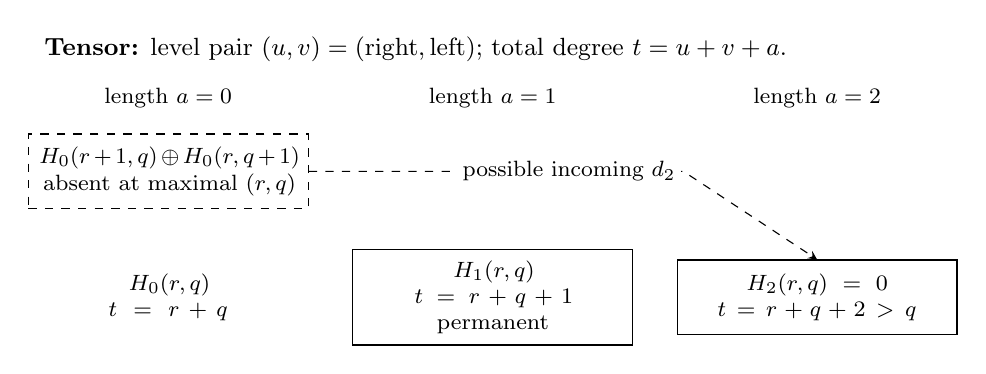
\begin{tikzpicture}[
      x=.01\linewidth,y=1cm,
      every node/.style={font=\footnotesize,align=center},
      term/.style={text width=.27\linewidth,inner sep=4pt},
      permanent/.style={term,draw,semithick,minimum height=.95cm},
      endpoint/.style={term,draw,thin,minimum height=.95cm},
      excluded/.style={term,draw,dashed,thin,minimum height=.95cm},
      differential/.style={->,thin,>=stealth}
    ]
    \node[anchor=west,align=left,font=\small] at (-14,0)
      {\textbf{Tensor:} level pair $(u,v)=(\text{right},\text{left})$;
        total degree $t=u+v+a$.};
    \node at (0,-.62) {length $a=0$};
    \node at (34,-.62) {length $a=1$};
    \node at (68,-.62) {length $a=2$};
    \node[excluded] (tensor-sources) at (0,-1.55)
      {$H_0(r+1,q)\oplus H_0(r,q+1)$\\
        absent at maximal $(r,q)$};
    \node[term] (tensor-zero) at (0,-3.15)
      {$H_0(r,q)$\\$t=r+q$};
    \node[permanent] (tensor-middle) at (34,-3.15)
      {$H_1(r,q)$\\$t=r+q+1$\\permanent};
    \node[endpoint] (tensor-two) at (68,-3.15)
      {$H_2(r,q)=0$\\$t=r+q+2>q$};
    \draw[differential,dashed] (tensor-sources.east)
      -- (54,-1.55) -- (tensor-two.north);
    \node[fill=white,inner sep=2pt] at (42,-1.55)
      {possible incoming $d_2$};

  \end{tikzpicture}
  \caption{The tensor length filtration at the highest contributing pair
    $(r,q)$.  The right normalized level is at most $r\ge-1$, and every
    contributing left color is in $T\cup\partial T$, where the cap is $q$.
    The only possible secondary differential is $d_2:0\to2$, so the middle
    classes are permanent.  Its two possible incoming sources at $(r,q)$
    are absent; hence the length-two classes also survive.  Their actual
    degree $r+q+2>q$ forces $H_2(r,q)=0$.  A residual right simple has
    normalized level $-1$ and assigned length $1$, which preserves the
    total-degree formula.  The dashed arrow marks an excluded possibility.
    Family and bidegree indices are suppressed.}
  \label{fig:filtrations}
\end{figure}


\begin{lemma}
\label{lem:two-point-remove-tops}
By replacing \(z\) within \(A_Jz\), preserving the cap on \(T\), one
can arrange that the highest normalized right layer has no right
top at any vertex of \(\widetilde J\).
\end{lemma}

\begin{proof}
Suppose a right top at the current highest level \(r\) occurs in
color \(j\in J\).  Lemma~\ref{lem:two-point-tensor-filtration} shows
that the left-family top in this color at level \(q\) vanishes.
The positive operation \(F_j\) therefore preserves the cap on
\(T\cup\partial T\), by Lemma~\ref{lem:cap-accessibility} applied
with spherical set \(T\).  Replace
\[
 z\longmapsto\sigma_jz,
 \qquad h\longmapsto h\sigma_j^{-1},
 \qquad R_\ell\longmapsto R_\ell B_{\sigma_j}^{-1}.
\]
The candidate, its harmonic vector \(p\), and the exterior cap are
unchanged.  The tensor products still compute the same complexes
\(U_\ell E_{L'}(z')\).  By
Lemma~\ref{lem:two-point-negative-bound}, the new maximum normalized
level is at most \(r\).  Thus the vanishing of the left top needed
to license the next move follows anew from
Lemma~\ref{lem:two-point-tensor-filtration}.

At a fixed value of \(r\), the sequence of chosen colors is reduced
in \(W_J\).  To prove this, let \(w\) be the reduced word already
chosen at this level.  If a color \(j\) were a right descent of
\(w\), a reduced expression for \(w\) could end in \(j\).
Matsumoto moves give the same negative Artin word in this
expression.  Each intermediate negative operation preserves the
upper bound \(r\), regardless of the expression.  The final inverse
operation in color \(j\) lowers the total test degrees in that
color by one.  Before it, every test above \(r+2\) vanishes; after
it, every test at \(r+2\) in color \(j\) therefore vanishes.
Formula~\eqref{eq:two-point-right-top} excludes a right top there.
A color selected for a nonzero right top must consequently be an
ascent, proving the assertion by induction on the number of moves.

The length of a reduced word in \(W_J\) is bounded by the length of
its longest element.  Therefore at a fixed \(r\) the procedure
either removes all the indicated tops or lowers the maximum level
after finitely many steps.  The maximum is an integer bounded below
by \(-1\), because the residual simples remain.  There are only
finitely many possible decreases from its initial value.  The
procedure terminates with the desired representative.  If
\(J=\varnothing\), no move is needed.
\end{proof}

\FloatBarrier
\subsection{Subrepresentations and the Euler estimate}

Use the representative supplied by
Lemma~\ref{lem:two-point-remove-tops}, and retain the notation
\(r,N,M\) for its highest right layer and left layer at \(q\).
Put
\[
 m=m^q(z),\qquad e=m-p.
\]
The vector \(e\) is supported on \(J\).  The cap on
\(T\cup\partial T\), together with the universal condition in
Definition~\ref{def:two-point-candidate}, verifies the hypotheses of
Proposition~\ref{prop:convex-subobjects} for \(A_Jz\).  Indeed, on
this coset the cap on \(T\setminus J\) is fixed, so a representative
capped on \(J\cup\partial J\) is also capped on \(T\).
Consequently \(e_J\) belongs to the convex hull of folded dimension
vectors \(s_J\) of families
\begin{equation}
\label{eq:two-point-subfamilies}
 \mathcal S_{L'}\subseteq M_{L'}
\end{equation}
of graded layer subrepresentations supported on \(\widetilde J\).
Their weighted dimensions have the form \(\phi s\), with \(s\)
zero outside \(J\).

\begin{lemma}
\label{lem:two-point-subrepresentation-tensor}
For every family \(\mathcal S\subseteq M\) in
\eqref{eq:two-point-subfamilies},
\begin{equation}
\label{eq:two-point-subrepresentation-homology}
 H_2(N,\mathcal S)=0,
 \qquad
 H_0(N,\mathcal S)\hookrightarrow H_0(N,M).
\end{equation}
\end{lemma}

\begin{proof}
The inclusion in degree zero follows from the inclusion of the
length-zero vector spaces and compatibility of the length-one
differentials.  Since there is no incoming term of negative length,
their degree-zero cohomologies are kernels, and kernel inclusion
gives the asserted injection.

For the degree-two assertion, work first with a single right row
and a single left subrepresentation, and retain homogeneous
coefficient spaces in their cochain gradings.  At every projective
vertex of \(\widetilde J\), vanishing of the right top says that
every right coefficient is a sum of incoming coefficient images,
from projective vertices or from the framing simple.  Iterating
this statement expresses coefficients in \(\widetilde J\) using
ones outside \(\widetilde J\) or in the simple: along an incoming
projective path the predecessor cochain placement is smaller by
one, and these placements are bounded below.

We make this iteration in the cokernel of the length-one
differential, rather than in the coefficient spaces alone.  Suppose
an incoming right coefficient at \(\beta\) comes from a homogeneous
coefficient at \(\gamma\), through a length-one map
\(Q_\gamma\to Q_\beta\).  Choose a middle path in
\(e_\gamma Z^1e_\beta\) dual to this arrow under the perfect
backtrack pairing.  Tensor this middle path with the coefficient
at \(\gamma\) and any homogeneous left coefficient in
\(\mathcal S_\beta\).  Its differential has two possible token
contributions.  The contribution at \(\beta\) is the selected
incoming right coefficient, tensored with the unchanged left
coefficient.  The contribution at \(\gamma\) is the original right
coefficient tensored with the corresponding left-arrow image, with
the ordinary cochain sign.  The dual path can be normalized so that
the first coefficient is one.  Hence, modulo length-two boundaries,
the token tensor at \(\beta\) is equal, up to a nonzero scalar and
sign, to the latter token tensor at \(\gamma\).

The new left coefficient lies in \(\mathcal S_\gamma\), since
\(\mathcal S\) is closed under the left coefficient maps.  Varying
the dual middle path tests every incoming arrow coefficient by
nondegeneracy of the pairing, including when an arrow space has
dimension greater than one.  Thus this substitution accounts for
the full span of incoming images.  Each substitution decreases the
right cochain placement by one and increases the left placement by
one, so the represented total degree is unchanged and the
substitution process terminates.

If it terminates at a projective vertex outside \(\widetilde J\),
the left coefficient is zero.  If an incoming coefficient comes
from the simple, its tensor with the same left coefficient is
itself an assigned length-one input.  The right differential sends
that tensor to exactly the token-inclusion image in question.  Its
left differential is zero because tensoring a radical left map
with a right simple gives zero.  Such a token tensor is therefore
already a boundary.  Every length-two generator is a sum of the
tensors just treated, so the cokernel vanishes.  This proves the
first assertion row by row and member by member, hence for the
families as well.
\end{proof}

Define the folded nonnegative vector \(n\), supported on \(T\), by
\begin{equation}
\label{eq:two-point-right-weight}
 n_j=\frac1{D_0}\sum_H w_H
       \sum_{i\in V'}\sum_L a'_i w_L
                K^r_{(i,L),(j,H)}(h)
       \qquad(j\in T).
\end{equation}
For any left-layer family of weighted dimension \(\phi y\), the
weighted Euler characteristic of its length complex with \(N\),
divided by \(D_0\), is
\begin{equation}
\label{eq:two-point-euler}
 \chi(n,y)=n^{\mathsf t}Cy
       -\mathbf1_{\{r=-1\}}(a')^{\mathsf t}y_T.
\end{equation}
Here is the count explicitly.  If
\[
 N_\beta^{\mathrm{wt}}
      =\sum_{i\in V'}\sum_L a'_i w_L K^r_{(i,L),\beta}(h),
\]
the projective part of the unnormalized count is
\[
 \sum_{\beta,\gamma}
       N_\beta^{\mathrm{wt}}\widetilde C_{\beta\gamma}(\phi y)_\gamma
   =\sum_{j,H}N_{(j,H)}^{\mathrm{wt}}w_H(Cy)_j
   =D_0 n^{\mathsf t}Cy.
\]
The two diagonal paths, of lengths zero and two, give diagonal
coefficient two; the middle arrows give minus adjacency.  We used
\(\widetilde C\phi=\phi C\) in the first equality.  If \(r=-1\),
the residual simples also occur at this level.  Their length-one
contribution is
\[
 -\sum_{i\in V'}\sum_L a'_i w_L\,(w_Ly_i)
      =-D_0(a')^{\mathsf t}y_T.
\]
No simple is present in \(N\) when \(r>-1\).  This proves
\eqref{eq:two-point-euler}, including its normalization and sign.

\begin{lemma}
\label{lem:two-point-euler-estimate}
At the representative with no highest right tops on \(J\),
\begin{equation}
\label{eq:two-point-estimate}
 \frac1{D_0}\dim_{\mathrm{wt}}H_1(N,M)
       \ge n_T^{\mathsf t}a
              +\mathbf1_{\{r=-1\}}(a')^{\mathsf t}p_T.
\end{equation}
\end{lemma}

\begin{proof}
For a family \(\mathcal S\) with folded dimension \(s\),
Lemma~\ref{lem:two-point-subrepresentation-tensor} and the Euler
identity give
\[
 \chi(n,s)
  =\frac{\dim_{\mathrm{wt}}H_0(N,\mathcal S)
             -\dim_{\mathrm{wt}}H_1(N,\mathcal S)}{D_0}
  \le\frac{\dim_{\mathrm{wt}}H_0(N,M)}{D_0}.
\]
The right side is independent of the chosen subfamily.  Since
\(e\) is a convex combination of these \(s\), and
\(\chi(n,\cdot)\) is linear, the same upper bound holds for
\(\chi(n,e)\).  On the other hand,
Lemma~\ref{lem:two-point-tensor-filtration} gives
\[
 \chi(n,m)
   =\frac{\dim_{\mathrm{wt}}H_0(N,M)
             -\dim_{\mathrm{wt}}H_1(N,M)}{D_0}.
\]
Subtracting yields
\[
 \frac1{D_0}\dim_{\mathrm{wt}}H_1(N,M)
    \ge\chi(n,e)-\chi(n,m)=-\chi(n,p).
\]
Finally, \(n\) is supported on \(T\), and \((Cp)_T=-a\).
Equation~\eqref{eq:two-point-euler} therefore turns the right side
into the expression in \eqref{eq:two-point-estimate}.
\end{proof}

\subsection{A spherical parabolic detector}

The tensor estimate is now available.  In the final comparison it will
force the harmonic vectors of two candidates to agree; to identify their
cosets as well, we need to recover parabolic membership from a vanishing
block of the right-projective counts \(K^r_{\ell\beta}\).

We need to reflect positive last-letter divisibility through the
finite unfolding.  Recall that a \emph{simple} positive element in a
finite-type Artin monoid is a reduced-word lift of an element of the
Coxeter group \(W_T\).
The finite-type monoid facts in
Theorem~\ref{thm:topology-finite-monoid} imply that the greatest simple
right divisor of a positive element \(b\) exists: it is its right gcd
with the Garside element.  Write it as \(t(b)\).

\begin{lemma}
\label{lem:two-point-greedy}
For nonidentity simple elements \(d_1,\ldots,d_k\), the factorization
\(d_1\cdots d_k\) is obtained by repeatedly extracting the greatest
simple suffix if and only if
\begin{equation}
\label{eq:two-point-greedy-condition}
 D_R(d_i)\subseteq D_L(d_{i+1})\qquad(1\le i<k).
\end{equation}
Here the descent sets are those of the corresponding elements of
the Coxeter group.  Consequently, if an unfolded vertex right-divides the
unfolding of a positive element of \(A_T^+\), its original color
right-divides that positive element.
\end{lemma}

\begin{proof}
An atom \(s\) right-divides a simple element \(d\) exactly when
\(s\in D_R(d)\), and \(sd\) is simple exactly when
\(s\notin D_L(d)\).  If the inclusion in
\eqref{eq:two-point-greedy-condition} fails, an atom in its difference
can be transferred from the end of \(d_i\) to the beginning of
\(d_{i+1}\), giving a larger simple suffix of the corresponding
prefix.  This proves necessity.

For sufficiency, induct on prefixes.  Suppose
\(P=d_1\cdots d_{j-1}\) has greatest simple suffix \(d_{j-1}\), and
let \(g=t(Pd_j)\).  Since \(d_j\) is a simple suffix, it right-divides
\(g\); write \(g=cd_j\).  If \(c\ne1\), choose a final atom of
\(c\), so \(c=c's\).  The element \(sd_j\), being a factor of the
simple element \(g\), is simple.  Also \(Pd_j=bg=bc d_j\) for some
positive \(b\), so cancellation gives \(P=bc\).  Thus \(s\)
right-divides \(P\).  Since an atom is simple, it right-divides
\(t(P)=d_{j-1}\).  We have obtained
\(s\in D_R(d_{j-1})\) and \(s\notin D_L(d_j)\), a contradiction.
Therefore \(g=d_j\), completing the induction.  Removing the final
factor successively gives the asserted greedy extraction.

Now take the greedy factorization of a positive original element.
Lemma~\ref{lem:finite-unfolding} says that reduced-word lifts remain
simple after unfolding, and that both descent sets become their full
color preimages.  Thus the unfolded factors satisfy
\eqref{eq:two-point-greedy-condition} and form the unfolded greedy
factorization.  Every extractable final atom of the unfolded element
right-divides its greatest simple suffix, hence is a right descent
of the last unfolded factor.  Descent reflection supplies its color
as a right descent of the last original factor.  That original atom
therefore right-divides the original positive element.
\end{proof}

The following detector uses successive common-divisor removal, as in
the proof of Brav--Thomas~\cite[Theorem~3.1]{BravThomas2011}.
Here the vanishing block of a family of right-simple tests yields a
specific parabolic subgroup; the unfolding step needed to recover
original colors is Lemma~\ref{lem:two-point-greedy}.

\begin{lemma}
\label{lem:parabolic-detection}
Let \(h\in A_T\) and \(\varnothing\ne V\subseteq T\).  If
\begin{equation}
\label{eq:two-point-zero-block}
 K^r_{\ell\beta}(h)=0
 \qquad
 (r\in\Zbb,\ \ell,\beta\in\widetilde V),
\end{equation}
then \(h\in A_{T\setminus V}\).
\end{lemma}

\begin{proof}
Fix \(\ell\in\widetilde V\).  The only right projective admitting a
nonzero map to or from \(U_\ell\) is \(Q_\ell\): a map to the simple
uses its top quotient, and a map from the simple uses its token
socle.  Condition~\eqref{eq:two-point-zero-block} excludes this
projective from \(R_\ell(h)\).  Its simple term therefore splits off
as a complex.  Tensoring with \(B_h\) is a homotopy equivalence and
preserves indecomposability.  Since \(U_\ell\) is indecomposable, the
remaining projective summand must be zero in the homotopy category.
It follows that
\[
 U_\ell B_h\simeq U_\ell\qquad(\ell\in\widetilde V).
\]

Use finite-type fractions to write \(h=h_1h_2^{-1}\) with
\(h_1,h_2\in A_T^+\).  On setting
\(U_V=\bigoplus_{\ell\in\widetilde V}U_\ell\), the preceding
equivalences give
\begin{equation}
\label{eq:two-point-equal-positive}
 U_V B_{h_1}\simeq U_V B_{h_2}.
\end{equation}
For a bounded right complex \(R\), use the height
\[
 \max\{t:H^t(Re_\beta)\ne0
                    \text{ for some }\beta\in\widetilde T\}
\]
from Lemma~\ref{lem:top-divisor}, with total cohomological degree as
there.  Its value on \(U_V\) is zero.  A positive word avoiding
\(V\) fixes \(U_V\).  If a positive word contains a color of \(V\),
all operations before its first such occurrence fix \(U_V\), and
that first occurrence acts on a highest test and raises the height.
The height cannot subsequently decrease.  Thus the final height is
positive exactly when the word contains a color of \(V\).

If the common height in \eqref{eq:two-point-equal-positive} is
positive, any vertex with highest cohomology gives, by the right
version of Lemma~\ref{lem:top-divisor}, an extractable final atom of
both unfolded positive words.  Lemma~\ref{lem:two-point-greedy}
supplies a common extractable original color \(s\).  Write
\(h_i=g_i\sigma_s\), and tensor
\eqref{eq:two-point-equal-positive} on the right by
\(B_{\sigma_s}^{-1}\).  This gives the same equality with \(g_i\)
in place of \(h_i\), while
\[
 h_1h_2^{-1}=g_1\sigma_s\sigma_s^{-1}g_2^{-1}=g_1g_2^{-1}.
\]
The sum of positive lengths decreases by two.  Repetition therefore
terminates with common height zero.  Both remaining positive words
then avoid \(V\), so their fraction lies in \(A_{T\setminus V}\).
\end{proof}

\subsection{Equality of candidates}

\begin{proof}[Proof of Proposition~\ref{prop:candidate-uniqueness}]
Suppose two candidates are given, and use the notation above.  Carry
out the top-removal procedure for the first candidate, with the
second supplying the positive row weights.  If its final highest
normalized right level satisfies \(r>-1\), that level contains a
nonzero projective coefficient and no framing simple.  It must
contain a nonzero coefficient in \(\widetilde V\).  Indeed, if it
were supported entirely on \(\widetilde J\), vanishing of all its
right tops there would express every coefficient using incoming
ones with strictly smaller cochain placement.  Boundedness would
force every coefficient to be zero.

All row weights are strictly positive.  A nonzero coefficient in
\(\widetilde V\) consequently gives \(n_i>0\) for some \(i\in V\).
Since \(a_i>0\) there, \(n_T^{\mathsf t}a>0\).
Equation~\eqref{eq:two-point-estimate} then gives nonzero middle
cohomology.  It survives in actual total degree \(r+q+1>q\),
contradicting \eqref{eq:two-point-actual-homology}.  We conclude that
\(r=-1\).

At this level the surviving middle cohomology lies in total degree
\(q\), so its weighted dimension is at most that of actual
cohomology there.  Since \(a'\) is supported on \(V'\), where
\(p'_i=m_i^q(z')\), equations
\eqref{eq:two-point-actual-homology} and
\eqref{eq:two-point-estimate} give
\begin{equation}
\label{eq:two-point-forward}
 (a')^{\mathsf t}(p'_T-p_T)
       \ge n_T^{\mathsf t}a\ge0.
\end{equation}
Interchanging the candidates and repeating the argument gives
\begin{equation}
\label{eq:two-point-reverse}
 a^{\mathsf t}(p_T-p'_T)\ge0.
\end{equation}
The two algorithms may choose different representatives.  The
vectors \(p,p',a,a'\), being data of the candidate cosets, are
unchanged by these choices.

The exterior coordinates of \(p\) and \(p'\) outside \(T\) agree.
Put \(\delta=p'_T-p_T\).  Then
\[
 a'-a=-C_T\delta.
\]
The sum of the left sides of \eqref{eq:two-point-forward} and
\eqref{eq:two-point-reverse} is therefore
\[
 (a'-a)^{\mathsf t}\delta
       =-\delta^{\mathsf t}C_T\delta.
\]
Both summands are nonnegative, whereas \(C_T\) is positive definite.
It follows that \(\delta=0\) and equality holds throughout.
Thus \(p=p'\), \(a=a'\), and
\[
 V=\{i\in T:a_i>0\}=V',\qquad J=J'.
\]
In particular the nonnegative term \(n_T^{\mathsf t}a\) in
\eqref{eq:two-point-forward} is zero.

It remains to identify the cosets, rather than just their numerical
data.  Fix the comparison element \(h_0=z'z^{-1}\) using any initial
representatives of the two candidates.  Replacing these by \(bz\)
and \(cz'\), with \(b\in A_J\) and \(c\in A_{J'}\), changes it to
\[
 c h_0 b^{-1}.
\]
By Lemma~\ref{lem:right-duality}, the block with row indices in
\(\widetilde V'\) and column indices in \(\widetilde V\) is
invariant under all such changes.  After the equality just proved,
this is the same block \(\widetilde V\times\widetilde V\) in both
directions.

In the forward comparison no right projective generator has degree
above \(-1\).  At degree \(-1\), the equality
\(n_T^{\mathsf t}a=0\), formula~\eqref{eq:two-point-right-weight},
and strict positivity of all its weights imply
\[
 K^{-1}_{\ell\beta}=0
       \qquad(\ell,\beta\in\widetilde V).
\]
Indeed every summand contributing to a column color in \(V\) has
a positive coefficient, and all counts are nonnegative.  By block
invariance, the fixed block for \(h_0\) is therefore zero in every
degree \(d\ge-1\).  The reverse comparison proves that the same
block for \(h_0^{-1}\) is zero for all \(d\ge-1\), irrespective of
the representatives chosen in that direction.  Formula
\eqref{eq:two-point-duality} transposes these latter vanishings into
vanishing of the block for \(h_0\) in all degrees \(d\le-1\).
Together the two ranges give
\[
 K^d_{\ell\beta}(h_0)=0
       \qquad(d\in\Zbb,\ \ell,\beta\in\widetilde V).
\]
Lemma~\ref{lem:parabolic-detection} gives
\(h_0\in A_{T\setminus V}=A_J\).  Thus
\(z'=h_0z\) and \(A_Jz'=A_Jz\), proving equality of the two
candidates.
\end{proof}

\section{The isolated harmonic-layer obstruction}
\label{sec:rigidity}

For a nonempty spherical type, we prove that prescribed null-vector data
outside it force some capped representative to meet a closed layer bound
inside it.
This supplies the nonemptiness of the closed sublevels used when a harmonic
height comparison has a null-vector tie.  Throughout this section,
$E_L=E_L(x)=B_xP_{o,L}$ denotes the family from
Section~\ref{sec:height-data}, and $Y_L^d$ denotes its pure layer of level $d$.
We retain both the cochain and internal gradings.  All signs below are
cochain signs.

\begin{proposition}[Isolated harmonic layer]
\label{prop:isolated-layer}
Let $I\subseteq S$ be nonempty and connected.  Let $c_I$ be a strictly
positive vector with $C_Ic_I=0$, and extend $c$ by zero on
$\widehat S\setminus I$.  Let $J\subseteq I$ be spherical, possibly
empty, let $q>0$ be an integer, and fix a coset $A_Jx$.  Suppose that the
fixed data on $(I\setminus J)\cup\partial I$ are capped at $q$ and
satisfy
\begin{equation}
 m^q|_{(I\setminus J)\cup\partial I}
   =c|_{(I\setminus J)\cup\partial I}.
 \label{eq:rigidity-exterior-data}
\end{equation}
It is impossible that every representative $z\in A_Jx$ capped at $q$ on
$I$ satisfies
\begin{equation}
 m_j^q(z)>c_j\qquad\text{for every }j\in J.
 \label{eq:rigidity-strict-hypothesis}
\end{equation}
Equivalently, if $J\ne\varnothing$ and
\eqref{eq:rigidity-exterior-data} holds, there is a representative capped
on $I$ and a color $j\in J$ with $m_j^q\le c_j$.  If $J=\varnothing$,
the exterior situation \eqref{eq:rigidity-exterior-data} itself is
impossible.
\end{proposition}

The proof assumes the strict inequalities at every capped representative.
Convex subobjects turn this hypothesis into an ordinary interior condition
on the excess of the level-$q$ multiplicities over $c$.  We then remove
socles from successive lower layers by positive twists, preserving the cap
and the conditions already established.  The Hom estimates below justify
these moves and force each
processed layer to avoid $\partial I$.  Since the frame contributes at
level zero, some layer below $q$ meets $\partial I$, giving the
contradiction.

\subsection{Linear Hom complexes and their three-column filtration}

Let $P$ and $Y$ be pure projective layers of levels $l$ and $k$, respectively.
For $i\in\{0,1,2\}$, let
$\mathcal L_i^{n,v}(P,Y)$ be the space of maps of path length $i$, cochain
degree $n$, and internal degree $v$.  Such a space can be nonzero only if
\begin{equation}
 n+v=k-l+i.
 \label{eq:rigidity-hom-degree}
\end{equation}
Indeed, a path-length-$i$ map between generators at placements $(c,u)$
and $(c',u')$ has degrees $n=c'-c$ and $v=u'+i-u$.
Write $\delta_P$ and $\delta_Y$ for the linear differentials of the layers.
The linear Hom differential is
\[
 D_1f=\delta_Yf-(-1)^n f\delta_P:
 \mathcal L_i^{n,v}(P,Y)\longrightarrow
 \mathcal L_{i+1}^{n+1,v}(P,Y).
\]
Put
\[
 \mathsf H_i^{n,v}(P,Y)=
 \frac{\ker\bigl(D_1|_{\mathcal L_i^{n,v}(P,Y)}\bigr)}
 {\operatorname{im}\bigl(D_1|_{\mathcal L_{i-1}^{n-1,v}(P,Y)}\bigr)},
 \qquad
 h_i(P,Y)=\sum_{n,v}\dim_{\C}\mathsf H_i^{n,v}(P,Y),
\]
where a space with path length outside $\{0,1,2\}$ is zero.  These sums are
finite, and the dimensions in them are unsigned.  In particular,
$\mathsf H_0$ has no boundaries: it consists of the homogeneous maps of
coefficient arrays commuting with the linear differentials up to the
indicated cochain sign.  The image of such a map is a graded
subrepresentation, after accounting for its placements.

\begin{lemma}[Hom pairing and middle vanishing]
\label{lem:rigidity-hom-filtration}
For pure projective layers $P,Y$, including those formed from graded
subrepresentations, there are perfect pairings
\[
 \mathsf H_i^{n,v}(P,Y)\ \times\
 \mathsf H_{2-i}^{-n,\,2-v}(Y,P)\longrightarrow\C.
\]
Consequently,
\begin{equation}
 \begin{split}
 h_2(P,Y)&=h_0(Y,P),\\
 (\dim P)^{\mathsf t}\widetilde C\,\dim Y
   &=h_0(P,Y)+h_0(Y,P)-h_1(P,Y).
 \end{split}
 \label{eq:rigidity-euler}
\end{equation}
Here $\dim P$ and $\dim Y$ count projective generators, with all placements
included.  For any two labels $L,H$ and any levels $l,k$,
\begin{equation}
 h_1(Y_L^l,Y_H^k)=0.
 \label{eq:rigidity-middle-vanishing}
\end{equation}
The same vanishing holds after replacing either layer by a direct summand
as a pure layer.
\end{lemma}

\begin{proof}
The symmetric Frobenius trace of $Z$, normalized by
$\operatorname{tr}(\theta_\alpha)=1$, pairs paths of length $i$ perfectly
with opposite paths of length $2-i$.  On complexes use the supertrace
\[
 \operatorname{Str}_Y(a)
   =\sum_c(-1)^c\operatorname{tr}(a|_{Y^c}).
\]
Here $Y^c$ denotes the cochain-degree-$c$ term, and the trace includes
the ordinary matrix trace on multiplicity spaces.  The
summandwise pairing
$\langle f,g\rangle=\operatorname{Str}_Y(f\circ g)$ is perfect between
$\mathcal L_i^{n,v}(P,Y)$ and
$\mathcal L_{2-i}^{-n,2-v}(Y,P)$.  Cyclicity gives, for the complementary
degrees appearing in a differential pairing,
\[
 \langle D_1f,g\rangle+(-1)^n\langle f,D_1g\rangle=0.
\]
There is no sign from the internal degree.  Finite-dimensional duality
therefore gives the asserted perfect pairings on cohomology.  This
argument uses only the linear differentials and the Frobenius pairing,
so it also applies to the pure layers associated with graded
subrepresentations.

The alternating sum of the dimensions of the three path-length columns
is $(\dim P)^{\mathsf t}\widetilde C\dim Y$: there are two equal-vertex
paths, of lengths zero and two, and the length-one paths contribute the
negative adjacency entries.  Euler characteristic and the pairing of
columns zero and two give \eqref{eq:rigidity-euler}.

For the remaining assertion, consider the full bigraded Hom complex
$\Hom_Z(E_L,E_H)$.  Minimality writes each projective differential as a
sum of its length-one and length-two parts.  Thus its Hom differential is
$D_1+D_2$, where $D_a$ raises path length by $a$.  Filter Hom by paths of
length at least $i$.  There are only the three columns $0,1,2$; the first
nonzero differential is $D_1$.  Its cohomology decomposes as the direct
sum of the spaces above, indexed by the ordered pair of source and target
layers.  After this page, the only possible differential goes from column
zero to column two.  Every column-one class is therefore permanent.

By Proposition~\ref{prop:twist-action}, applying $B_x$ preserves the
bigraded Hom cohomology.  Between the initial frame projectives this
cohomology is zero when $L\ne H$.  When $L=H$, it has dimension one in each
of bidegrees $(0,0)$ and $(0,2)$ and is zero elsewhere.  Both of these
dimensions have specific permanent representatives in the filtration.
First, the identity of $E_L$ is a nonzero class in column zero and bidegree
$(0,0)$; a boundary cannot have a length-zero component.  Second, choose
one projective summand in the nonzero minimal complex $E_L$, and place its
normalized token on that diagonal matrix entry, with all other entries
zero.  This is a cycle in bidegree $(0,2)$, since a token multiplied on
either side by a radical entry is zero.  If the chosen summand is in
cochain placement $c$, this cycle has supertrace $(-1)^c\ne0$.
Every Hom boundary has zero supertrace by graded cyclicity, so the token
cycle is nonzero in actual Hom cohomology.  It lies in filtration two,
and filtration three is zero; hence it supplies a nonzero column-two
class in the associated graded cohomology.

The identity and token exhaust the two actual diagonal Hom dimensions.
All actual off-diagonal Hom cohomology vanishes.  Since every column-one
class is permanent, every such class must be zero, proving
\eqref{eq:rigidity-middle-vanishing}.  Finally, a direct summand of a pure
layer gives a direct summand of each linear Hom complex.  Its column-one
cohomology is therefore zero as well.  This last argument is on the
linear page; it does not assert that the chosen layer summand splits off
from the full complex $E_L$.
\end{proof}

The numerical identity \eqref{eq:rigidity-euler} parallels
Crawley--Boevey's Hom--Ext formula for preprojective modules
\cite[Lemma~1]{CrawleyBoevey2000}.

We will also use weighted versions of these formulas.  For families
$\mathcal P=(P_L)_L$ and $\mathcal Y=(Y_H)_H$, define the nonnegative real
number
\[
 h_i^{\mathrm{wt}}(\mathcal P,\mathcal Y)
   =\sum_{L,H}w_Lw_H h_i(P_L,Y_H).
\]
These are weighted dimensions, not necessarily integer dimensions of
vector spaces.  If the two weighted generator arrays are $\phi p$ and
$\phi y$, respectively, then
\[
 \sum_{L,H}w_Lw_H
 (\dim P_L)^{\mathsf t}\widetilde C\dim Y_H
   =(\phi p)^{\mathsf t}\widetilde C\phi y
   =D_0p^{\mathsf t}Cy,
 \qquad D_0=\sum_Lw_L^2.
\]
The symmetry of $w_Lw_H$ under interchange of the labels gives
\begin{equation}
 D_0p^{\mathsf t}Cy
   =h_0^{\mathrm{wt}}(\mathcal P,\mathcal Y)
    +h_0^{\mathrm{wt}}(\mathcal Y,\mathcal P)
    -h_1^{\mathrm{wt}}(\mathcal P,\mathcal Y).
 \label{eq:rigidity-weighted-euler}
\end{equation}

\begin{lemma}[The capped secondary injection]
\label{lem:rigidity-secondary-injection}
Let $I\subseteq S$, and suppose the family $E_L$ is capped at $q$ on $I$.
For every $L$, let $M_L$ be a direct summand of the pure layer $Y_L^q$
supported on $\widetilde I$.  If $d<q$, then for every pair of labels $L,H$
there are injections
\begin{equation}
 \mathsf H_0^{n,v}(M_L,Y_H^d)
   \lhook\joinrel\longrightarrow
 \mathsf H_2^{n+1,v}(M_L,Y_H^{d-1}),
 \qquad n+v=d-q.
 \label{eq:rigidity-secondary-injection}
\end{equation}
In particular, for $\mathcal M=(M_L)_L$ and
$\mathcal Y^d=(Y_H^d)_H$,
\begin{equation}
 h_0^{\mathrm{wt}}(\mathcal M,\mathcal Y^d)
 \le h_0^{\mathrm{wt}}(\mathcal Y^{d-1},\mathcal M).
 \label{eq:rigidity-secondary-bound}
\end{equation}
\end{lemma}

\begin{proof}
Represent a class on the left of
\eqref{eq:rigidity-secondary-injection} by a homogeneous length-zero
linear cocycle $f$, and extend it by zero on the other source-layer
summands.  This is a linear cocycle in $\Hom_Z(E_L,E_H)$ because $M_L$ is
a direct summand for the linear differential.  It defines an embedded
column-zero class on the page after $D_1$: the linear differential
preserves the ordered source/target layer pair, and column zero has no
incoming boundaries.

Write the length-two projective differentials as $d_{E_L}^{(2)}$ and
$d_{E_H}^{(2)}$.  The secondary differential on this class is represented
by
\[
 d_{E_H}^{(2)}f-(-1)^n f d_{E_L}^{(2)}.
\]
The only possible ordered layer pairs in its target are
\begin{equation}
 \begin{array}{ccl}
 (q,d-1)&\text{from}&d_{E_H}^{(2)}f,\\
 (q+1,d)&\text{from}&f d_{E_L}^{(2)}.
 \end{array}
 \label{eq:rigidity-secondary-blocks}
\end{equation}
A length-two entry is diagonal in the unfolded vertex and lowers the
layer by one.  For the second term in
\eqref{eq:rigidity-secondary-blocks} to be nonzero, its source would have
to lie at level $q+1$ on a vertex of $\widetilde I$.  Such generators are
excluded by the cap.  Vertices outside $\widetilde I$ cannot contribute
through a diagonal length-two entry.  Thus the secondary image lies
entirely in the first block.  The splitting $Y_L^q=M_L\oplus M_L^{\prime}$
is a splitting for the linear differential, so it splits the target
column-two cohomology by source summands as well.  The target-side
composite is zero on $M_L^{\prime}$ and therefore lands in the summand
$\mathsf H_2(M_L,Y_H^{d-1})$, giving the map in
\eqref{eq:rigidity-secondary-injection}.

If a class were in its kernel, it would be permanent: no differential
enters column zero, and there is no possible differential after the
secondary one.  Its total degree is $d-q<0$.  Actual Hom cohomology between
$E_L$ and $E_H$ is zero in this degree by the computation in
Lemma~\ref{lem:rigidity-hom-filtration}.  The class is therefore zero.
This proves the injection for each pair of labels before any weighting.
Sum the resulting dimension inequalities with positive weights $w_Lw_H$
and use the dual pairing of
Lemma~\ref{lem:rigidity-hom-filtration}; the result is
\eqref{eq:rigidity-secondary-bound}.
\end{proof}

Figure~\ref{fig:hom-filtration} records the two possible secondary
targets.  The tensor estimate in Figure~\ref{fig:filtrations} excluded
an incoming secondary differential at a maximal pair of levels.  Here the
cap removes one outgoing term, so negative-degree Hom vanishing forces
injection into the other target.

\begin{figure}[tbp]
  \centering
  {\small
    Linear part: $C_0\xrightarrow{d_1}C_1\xrightarrow{d_1}C_2$,
    \quad $H_a=H^a(C_\bullet,d_1)$.\par}
  \medskip
  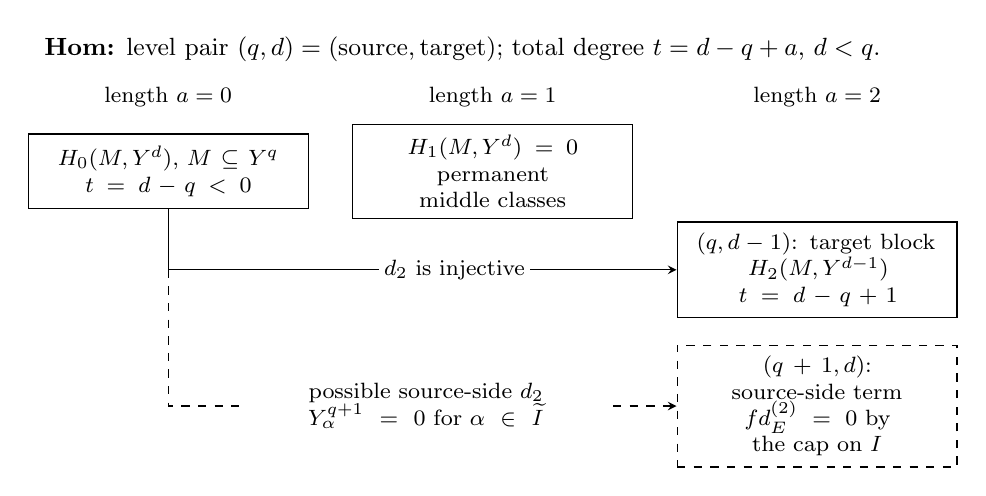
\begin{tikzpicture}[
      x=.01\linewidth,y=1cm,
      every node/.style={font=\footnotesize,align=center},
      term/.style={text width=.27\linewidth,inner sep=4pt},
      permanent/.style={term,draw,semithick,minimum height=.95cm},
      endpoint/.style={term,draw,thin,minimum height=.95cm},
      excluded/.style={term,draw,dashed,thin,minimum height=.95cm},
      differential/.style={->,thin,>=stealth}
    ]
    \node[anchor=west,align=left,font=\small] at (-14,-4.55)
      {\textbf{Hom:} level pair $(q,d)=(\text{source},\text{target})$;
        total degree $t=d-q+a$, $d<q$.};
    \node at (0,-5.16) {length $a=0$};
    \node at (34,-5.16) {length $a=1$};
    \node at (68,-5.16) {length $a=2$};
    \node[endpoint] (hom-zero) at (0,-6.1)
      {$H_0(M,Y^d)$, $M\subseteq Y^q$\\$t=d-q<0$};
    \node[permanent] (hom-middle) at (34,-6.1)
      {$H_1(M,Y^d)=0$\\permanent middle classes};
    \node[endpoint] (hom-target) at (68,-7.35)
      {$(q,d-1)$: target block\\$H_2(M,Y^{d-1})$\\$t=d-q+1$};
    \node[excluded] (hom-source) at (68,-9.08)
      {$(q+1,d)$: source-side term\\$f d_E^{(2)}=0$ by the cap on $I$};
    \draw[differential] (hom-zero.south) -- (0,-7.35)
      -- (hom-target.west);
    \node[fill=white,inner sep=2pt] at (30,-7.35)
      {$d_2$ is injective};
    \draw[differential,dashed] (0,-7.35) -- (0,-9.08)
      -- (hom-source.west);
    \node[fill=white,text width=.38\linewidth,inner sep=2pt] at (27,-9.08)
      {possible source-side $d_2$\\
        $Y^{q+1}_\alpha=0$ for $\alpha\in\widetilde I$};
  \end{tikzpicture}
  \caption{The Hom length filtration for a direct summand $M$ of $Y^q$
    supported on $\widetilde I$, with the family capped at $q$ on $I$.
    Here $d<q$, and $H_a$ denotes the linear cohomology $\mathsf H_a$ with
    family and bidegree indices suppressed.  The secondary differential
    of a length-zero linear cocycle $f$ has the two displayed target blocks;
    $d_E^{(2)}$ denotes the length-two part of the source differential.
    The source-side contribution
    $f d_E^{(2)}$ vanishes: length-two paths are diagonal and the cap
    excludes level-$q+1$ source generators on $\widetilde I$.
    Higher source generators outside $I$ need not vanish.
    Negative-degree actual Hom vanishes, forcing injection into the
    remaining target block.  The identity and token classes give the
    middle vanishing proved in Lemma~\ref{lem:rigidity-hom-filtration}.
    The dashed arrow marks an excluded possibility.}
  \label{fig:hom-filtration}
\end{figure}


\subsection{Convex subrepresentations and the boundary sign}

The following consequence of the Hom calculation isolates the convex
part of the argument.  For a family of layers, saying that its socle
vanishes on a color set means that this holds at every unfolded vertex
of those colors in every member of the family.

\begin{lemma}[Separation from the boundary]
\label{lem:rigidity-separation}
Let $I\subseteq S$ be nonempty and connected, and let $c$ be zero off $I$
and strictly positive on $I$, with $C_Ic_I=0$.  Let $J\subseteq I$.
Suppose $\mathcal M=(M_L)_L$ is a family of direct summands of one pure
layer of the family $E_L$, supported on $\widetilde I$, with weighted
generator array $\phi m$.  Assume $m-c$ is supported on $J$ and that
$(m-c)_J$ is an interior point in $\R^J$ of the convex hull of finitely
many vectors $s_J$ with the following properties: $s$ is zero off $J$,
and $\phi s$ is the weighted generator array of a family of graded
subrepresentations $\mathcal S=(S_L)_L\subseteq\mathcal M$ supported on
$\widetilde J$.

Let $\mathcal Y=\mathcal Y^d$ be any layer of the family $E_L$, and write
$\phi y$ for its weighted generator array.  If its socle vanishes on $J$,
then
\begin{equation}
 y|_{\partial I}=0,\qquad
 (Cy)_J=0,\qquad
 h_0^{\mathrm{wt}}(\mathcal M,\mathcal Y)
 =h_0^{\mathrm{wt}}(\mathcal Y,\mathcal M)=0.
 \label{eq:rigidity-separation-conclusions}
\end{equation}
Here $\partial I$ is the outside-neighbor set, including the frame.
The assertion includes the usual interior convention in $\R^0$ when
$J=\varnothing$.
\end{lemma}

\begin{proof}
Fix one of the subrepresentation families $\mathcal S$.  A nonzero
homogeneous coefficient-array map $S_L\to Y_H$ has a nonzero graded
image supported on $\widetilde J$.  Such an image has a socle: arrow
coefficients raise cochain placement, so a nonzero coefficient in its
highest occupied placement is killed by every outgoing arrow.  Since
the image is a subrepresentation, this is a socle of $Y_H$ on
$\widetilde J$.  The hypothesis therefore gives
\[
 h_0^{\mathrm{wt}}(\mathcal S,\mathcal Y)=0.
\]
Also, composition with the inclusion $S_L\hookrightarrow M_L$ gives
injections on length-zero linear cocycles, with no length-zero
boundaries to quotient out.  Thus
\[
 h_0^{\mathrm{wt}}(\mathcal Y,\mathcal S)
 \le h_0^{\mathrm{wt}}(\mathcal Y,\mathcal M).
\]
Apply \eqref{eq:rigidity-weighted-euler} first to
$(\mathcal S,\mathcal Y)$ and then to $(\mathcal M,\mathcal Y)$.
The first application uses only
$h_1^{\mathrm{wt}}(\mathcal S,\mathcal Y)\ge0$; the second has
$h_1^{\mathrm{wt}}(\mathcal M,\mathcal Y)=0$ by
Lemma~\ref{lem:rigidity-hom-filtration}.  Subtracting gives
\begin{equation}
 D_0(m-s)^{\mathsf t}Cy
 \ge h_0^{\mathrm{wt}}(\mathcal M,\mathcal Y)\ge0.
 \label{eq:rigidity-convex-inequality}
\end{equation}
In particular, no middle-Hom vanishing for $\mathcal S$ is required.

The left side of \eqref{eq:rigidity-convex-inequality} is affine-linear
in $s$, so the inequality holds throughout the convex hull.  At its
interior point $e=m-c$, it gives
\begin{equation}
 D_0c^{\mathsf t}Cy
 \ge h_0^{\mathrm{wt}}(\mathcal M,\mathcal Y)\ge0.
 \label{eq:rigidity-null-average}
\end{equation}
On the other hand, symmetry of $C$, the null equation on $I$, and
nonnegativity of $y$ give
\begin{equation}
 c^{\mathsf t}Cy
  =-\sum_{a\notin I}\sum_{i\in I}b_{ai}c_i y_a\le0.
 \label{eq:rigidity-boundary-sign}
\end{equation}
This is strictly negative if $y_a>0$ for any $a\in\partial I$.
Consequently $y|_{\partial I}=0$, the two sides of
\eqref{eq:rigidity-null-average} are zero, and
$h_0^{\mathrm{wt}}(\mathcal M,\mathcal Y)=0$.

Because $e_J$ is an ordinary real interior point, for each $j\in J$ the
hull contains $e_J\pm\varepsilon\mathbf e_j$ for sufficiently small
$\varepsilon>0$.  Substituting these two points into
\eqref{eq:rigidity-convex-inequality}, whose value at $e$ is now zero,
forces $(Cy)_j=0$.  It follows that
\[
 m^{\mathsf t}Cy
   =c^{\mathsf t}Cy+(m-c)_J^{\mathsf t}(Cy)_J=0.
\]
The weighted Euler identity, with middle vanishing for $\mathcal M$,
now forces $h_0^{\mathrm{wt}}(\mathcal Y,\mathcal M)=0$ as well.
When $J=\varnothing$, one has $m=c$ and the hull is the singleton in
$\R^0$; the same argument applies with no coordinate perturbations.
\end{proof}

\subsection{The socle-removal induction}

\begin{proof}[Proof of Proposition~\ref{prop:isolated-layer}]
Assume \eqref{eq:rigidity-strict-hypothesis} holds at every capped
representative.  Since
$\partial J\subseteq(I\setminus J)\cup\partial I$,
Lemma~\ref{lem:cap-accessibility} supplies a representative capped on $J$
and hence on all of $I$.  We shall move only among such representatives.
All the exterior data in \eqref{eq:rigidity-exterior-data} stay fixed,
since operations in $A_J$ change multiplicities only in colors of $J$.

At any capped representative, let $M_L$ be the part of $Y_L^q$ supported
on $\widetilde I$, and set $\mathcal M=(M_L)_L$.  This is a direct
summand of the pure layer: its outside neighbors have zero multiplicity
at level $q$ by \eqref{eq:rigidity-exterior-data}, so no linear arrow
joins it to the rest of that layer.  This statement concerns the pure
layer, and does not assert a splitting of $E_L$.  By
Lemma~\ref{lem:family-proportionality}, its weighted generator array is
$\phi m$, where $m$ equals $m^q$ on $I$ and is zero off $I$.

Harmonizing the full level-$q$ vector on $J$ gives the coordinates $c_J$.
Indeed, only neighbors of $J$ enter these equations, their prescribed
values are those of $c$, and $C_Ic_I=0$; uniqueness follows from the
sphericity of $J$.  Remote coordinates outside $I\cup\partial I$ do not
enter these equations.  Capping a representative on $J$, with the fixed
exterior cap, is equivalent to capping it on $I$.
Proposition~\ref{prop:convex-subobjects} therefore applies with its strict,
universally quantified hypothesis.  It shows that
\begin{equation}
 e=m-c,\qquad \supp(e)\subseteq J,
 \qquad
 e_J\in\operatorname{int}_{\R^J}
 \operatorname{conv}\{s_J\},
 \label{eq:rigidity-interior}
\end{equation}
where each $s$ is the folded weighted dimension of subrepresentations
$\mathcal S\subseteq\mathcal M$ supported on $\widetilde J$.
Such subrepresentations, initially obtained in the full layer, lie in
$\mathcal M$ because of their support.

The interior in \eqref{eq:rigidity-interior} is the ordinary real
interior supplied by Proposition~\ref{prop:convex-subobjects}, even when
folded multiplicities are not integers.  For $J=\varnothing$, it means
$e=0$ in $\R^0$.

Thus Lemma~\ref{lem:rigidity-separation} applies at every capped
representative.  This uniformity is essential: both $\mathcal M$ and its
convex hull may change during the following operations, but the
hypothesis \eqref{eq:rigidity-strict-hypothesis} supplies
\eqref{eq:rigidity-interior} anew after each cap-preserving move.

Let $d_b$ be the lowest layer that meets $\partial I$.  This level exists
because the frame $o$ belongs to $\partial I$ and $m_o^0=1$.  It is fixed
throughout the coset, and
\begin{equation}
 d_b\le0<q.
 \label{eq:rigidity-boundary-level}
\end{equation}
Choose an integer $d_{\min}$ below or equal to every initially occupied
layer of every member of the family.  Positive operations cannot create
layers below $d_{\min}$ by their amplitude.  We shall proceed through
$d=d_{\min},\ldots,d_b$.  At the beginning of a stage, the induction
conditions are, for every $k<d$,
\begin{equation}
 \begin{aligned}
 \operatorname{soc}_{\widetilde J}\mathcal Y^k&=0,
 & (Cm^k)_J&=0,\\
 h_0^{\mathrm{wt}}(\mathcal Y^k,\mathcal M)&=0,
 & h_0^{\mathrm{wt}}(\mathcal M,\mathcal Y^k)&=0.
 \end{aligned}
 \label{eq:rigidity-induction}
\end{equation}
Here $m^k$ is the folded vector of the full layer $\mathcal Y^k$, and
$\mathcal M$ always denotes the current level-$q$ summand.  The conditions
hold initially since all lower layers are zero.

Since $d\le d_b<q$, Lemma~\ref{lem:rigidity-secondary-injection} and the
condition at $d-1$ give
\begin{equation}
 h_0^{\mathrm{wt}}(\mathcal M,\mathcal Y^d)=0.
 \label{eq:rigidity-current-hom-zero}
\end{equation}
Suppose that $\mathcal Y^d$ has a nonzero socle in a color $j\in J$.
Then $\mathcal M$ has zero top in that color.  To see this, a top simple
quotient of some $M_L$ and a socle simple of some $Y_H^d$ at the same
unfolded vertex compose to a nonzero homogeneous length-zero map.
Lemma~\ref{lem:family-proportionality} ensures that if a top occurs
anywhere in color $j$ in the family, then it occurs at every label in
that color in some family member.  It can therefore be matched with the
label of the chosen socle.  The resulting map would contradict
\eqref{eq:rigidity-current-hom-zero}, since every weight is positive.

Apply $F_j$ to this representative.  The top of $\mathcal M$ at color
$j$ is the top of the full level-$q$ layer there, because $\mathcal M$ is
a direct summand containing that color.  Its vanishing makes this move
cap-preserving by Lemma~\ref{lem:cap-accessibility}.  Concretely, the only
new level-$q+1$ contribution from the level-$q$ layer is this top; higher
layers have no generators on $I\cup\partial I$, and the twist acts
identically on that remote part.  Other colors keep their multiplicities.

We next prove that this move preserves
\eqref{eq:rigidity-induction} and changes the level-$d$ layer only by its
unshifted positive operation.  Denote the data immediately before and
after the move by ``old'' and ``new''.  For this single move, ascend again
through the integers $k<d$, starting below all occupied layers.  Suppose
that the old top at color $j$ in level $k-1$ has already been shown to
vanish.  This is vacuous at the starting level.
Lemma~\ref{lem:layers-amplitude-extension} then identifies
\begin{equation}
 \mathcal Y^k_{\mathrm{new}}
   \cong\text{the level-$k$ part of }F_j\mathcal Y^k_{\mathrm{old}}.
 \label{eq:rigidity-unshifted-step}
\end{equation}
Indeed, the level-$k$ term from the old level $k-1$ is exactly its top in
color $j$, and no other input layer contributes at $k$.  By
Lemma~\ref{lem:positive-layer}, the vanishing of the old socle on $J$
implies the vanishing of the new socle on $J$ in
\eqref{eq:rigidity-unshifted-step}.

The new representative is capped, so
Lemma~\ref{lem:rigidity-separation} applies using its new family
$\mathcal M_{\mathrm{new}}$.  As $k<d\le d_b$, the layer has no boundary
support.  The lemma yields all the new conditions
\eqref{eq:rigidity-induction} at this $k$, including
$(Cm^k_{\mathrm{new}})_j=0$.  The old row is also zero, and all
multiplicities off color $j$ are unchanged.  Since $C_{jj}=2$, comparison
of the two rows gives
\[
 2\bigl(m^k_{\mathrm{new},j}-m^k_{\mathrm{old},j}\bigr)=0.
\]
Let $t_j^k\ge0$ be the folded weighted top multiplicity of
$\mathcal Y^k_{\mathrm{old}}$ in color $j$.  Formula
\eqref{eq:layers-positive-dimension}, together with
\eqref{eq:rigidity-unshifted-step}, says
\[
 m^k_{\mathrm{new},j}
   =m^k_{\mathrm{old},j}-(Cm^k_{\mathrm{old}})_j+t_j^k.
\]
Thus $t_j^k=0$.  Positivity of the weights makes every old top in this
color zero, providing the premise at $k+1$.  This completes the upward
verification.  In particular, the old top at level $d-1$ is zero, so
\eqref{eq:rigidity-unshifted-step} also holds at $k=d$.

The order of this verification is important: the absence of a shifted-in
contribution at $k$ uses the top vanishing already established at $k-1$;
the top vanishing at $k$ is then deduced from the new row equation and the
pure-layer dimension formula.  Hence no assertion about the level being
checked is assumed in advance.  The verification also proves that
\eqref{eq:rigidity-current-hom-zero} can be used again after the move,
with the new $\mathcal M$, by
Lemma~\ref{lem:rigidity-secondary-injection}.

Continue applying $F_j$ whenever a socle in a color $j\in J$ remains in
level $d$.  This process terminates.  To prove it, consider only the
unshifted operations on that fixed pure layer.  By
Lemma~\ref{lem:layers-bottom-composition}, a composite is the bottom
cohomology of the corresponding positive word, so these operations
satisfy the positive braid relations.  A last-action color has zero
socle after its operation by Lemma~\ref{lem:positive-layer}.
Inductively suppose the colors used so far form a reduced expression
for $w\in W_J$, with the most recent operation written on the left.  If
the next chosen color $j$ were a left descent of $w$, a reduced
expression for $w$ would begin with $j$.  Braid moves would therefore
express the current pure layer as the result of an unshifted $F_j$
operation acting last.  Its socle in color $j$ would be zero,
contradicting the choice of $j$.  Each choice is consequently a Coxeter
ascent.  Since $W_J$ is finite, the number of choices at level $d$ is
bounded by the length of its longest element.

At termination, the socle on $J$ vanishes in the current layer $d$.
If $d<d_b$, Lemma~\ref{lem:rigidity-separation} supplies
\eqref{eq:rigidity-induction} also at $k=d$, and we proceed to the next
level.  The range from $d_{\min}$ to $d_b$ is finite, and the earlier
conditions were preserved during every move.  At $d=d_b$, the same
lemma asserts that the layer has no support on $\partial I$, contradicting
the definition of $d_b$.

If $J=\varnothing$, the procedure contains no firing steps: the socle
condition on $J$ is vacuous, \eqref{eq:rigidity-interior} says $m=c$, and
Lemma~\ref{lem:rigidity-separation} already contradicts the boundary
layer.  Thus the dimension-zero case is included.  The contradiction
proves the proposition.
\end{proof}

\section{Sublevels in spherical residues}
\label{sec:residues}

Inside a spherical coset, we consider smaller cosets whose exposed layer
counts lie below the ambient harmonic vector.  The two-point estimate will
show that a nonempty sublevel has only one source in its vertex filtration.
The isolated-layer obstruction has a different role: for the closed
inequalities associated with a positive null vector, it guarantees
nonemptiness and excludes the rank-zero exterior data.  We begin with the
topological principle that converts the link calculations into
contractibility.

\begin{lemma}[Vertex filtration]
\label{lem:filtration-principle}
Let $\mathcal P$ be a set-sized poset, and well-order its elements by
$\prec$.  For $v\in\mathcal P$, define the earlier lower and upper posets
\[
 \mathcal L_v=\{w\in\mathcal P:w<v,\ w\prec v\},\qquad
 \mathcal U_v=\{w\in\mathcal P:v<w,\ w\prec v\}.
\]
The link along which $v$ is added to the induced order complex on its
predecessors is the simplicial join of the order complexes of
$\mathcal L_v$ and $\mathcal U_v$.  If one poset is empty, this link is
the order complex of the other; if both are empty, the link is empty.

Suppose each attaching link is empty or contractible.  Then every
component of $|\mathcal P|$ is contractible and contains exactly one
\emph{source}, meaning a vertex with empty attaching link.  In
particular, the conclusion holds if each of $\mathcal L_v$ and
$\mathcal U_v$ is empty or contractible for every $v$.
\end{lemma}

\begin{proof}
A chain containing $v$ consists of a chain below $v$, the vertex $v$,
and a chain above $v$.  Every element of the first chain precedes every
element of the second in the poset order.  Restricting all other vertices
to those earlier than $v$ proves the asserted join description.  The
join of two nonempty contractible complexes is contractible.  Together
with the stated conventions for empty factors, this proves the last
assertion from the first one.

Index the vertices as $v_\alpha$, $\alpha<\kappa$, and let $K_\alpha$
be the induced order complex on $\{v_\beta:\beta<\alpha\}$.  At a
successor stage we attach the cone on the earlier link $L_\alpha$:
\[
 K_{\alpha+1}=K_\alpha\cup_{L_\alpha}(v_\alpha*L_\alpha).
\]
An empty link adds an isolated vertex and starts one component.  A
nonempty contractible link lies in a single component of $K_\alpha$.
The inclusion of that link in its cone is a homotopy equivalence and
a subcomplex cofibration.  The homotopy extension property therefore
makes the induced inclusion of the old component into the new one a
homotopy equivalence.  No other component changes, and two old
components cannot merge.  Thus the asserted description of components
and their sources persists at successor stages.

At a limit ordinal $\lambda$, the complex is the union of the earlier
subcomplexes, with the CW topology.  We recall why compact images cause
no difficulty in this union.  A compact subset of a closure-finite CW
complex lies in a finite subcomplex.  Otherwise it meets infinitely many
open cells; choose one point in each of a countable set of these cells.
Every subset of the chosen points meets each closed cell in a finite
set, by closure-finiteness, and hence is closed in the whole complex by
the weak topology.  The chosen points would therefore form an infinite
closed discrete subspace of the compact subset, a contradiction.  The
closures of the finitely many cells met by a compact subset form the
required finite subcomplex.

Consequently a path or a sphere map in $K_\lambda$ has image in some
$K_\alpha$ with $\alpha<\lambda$: only finitely many vertex indices
occur in its finite carrier.  Paths cannot merge previously distinct
components at the limit.  Every sphere map within a component is
null-homotopic in an earlier component, which is contractible by
induction.  Each component of $K_\lambda$ is thus weakly contractible
and has the same unique source as any of its earlier vertices.
Components are CW subcomplexes, so the CW Whitehead theorem makes them
contractible.  Transfinite induction, including the final union,
proves the result.
\end{proof}

We will also use the order homotopy observation that an order map
$f:\mathcal P\to\mathcal P$ satisfying $f(x)\le x$ for every $x$, or
$f(x)\ge x$ for every $x$, induces a map homotopic to the identity.
For example, when $f(x)\le x$, the assignments
$(x,0)\mapsto f(x)$ and $(x,1)\mapsto x$ form an order map from
$\mathcal P\times\{0<1\}$: if $x\le y$, then $f(x)\le y$.
The usual prism triangulation on every chain gives the homotopy, and
these homotopies agree on faces.  Thus an order retraction pointwise
comparable with the identity is a homotopy equivalence on order
complexes.  A poset with a maximum has a conical order complex.

\subsection{The two local sublevels}

Fix a spherical subset $T\subseteq S$, an integer $q$, and a right
coset $A_Tx$.  Assume that the layer data are capped at $q$ on
$\partial T$.  Operations in $A_T$ leave all exterior data unchanged,
so this assumption is independent of the representative.  Let $b$ be
the full vector obtained from $m^q(x)$ by harmonic extension on $T$:
\[
 b_i=m_i^q(x)\quad(i\notin T),\qquad (Cb)_T=0.
\]
The vector $b$ is nonnegative and independent of $x$ within its coset.
Here and throughout, caps concern all levels greater than $q$, whereas
the displayed inequalities concern level $q$ alone.

Consider pairs
\begin{equation}
 \label{eq:residues-pairs}
 X=(J,A_Jz),\qquad J\subsetneq T,\qquad z\in A_Tx,
\end{equation}
ordered by nested types and actual inclusion of cosets.  The open
colors of $X$ are $V=T\setminus J$.  Counts and caps on $V$ are
well-defined on $A_Jz$, since operations in $A_J$ change data only
in colors of $J$.

The \emph{strict sublevel} $\mathcal R_{<}(T,A_Tx;q)$ consists of
the pairs in \eqref{eq:residues-pairs} for which every $i\in V$ is
capped at $q$ and satisfies
\begin{equation}
 \label{eq:residues-strict}
 m_i^q(z)<b_i.
\end{equation}
We use a closed sublevel only with the following additional data:
\begin{enumerate}[label=(\roman*)]
 \item $q>0$;
 \item $I\subseteq S$ is nonempty and connected, with $T\subseteq I$;
 \item $c_I>0$ and $C_Ic_I=0$, and $c$ is extended by zero outside $I$;
 \item on $(I\setminus T)\cup\partial I$ the data are capped at $q$
 and satisfy $m^q=c$.
\end{enumerate}
These are exterior conditions for $A_Tx$.  In particular they imply
the assumed cap on $\partial T$.  Harmonicity and uniqueness of
extension give $b_T=c_T$.  The \emph{special closed sublevel}
$\mathcal R_{\le}(T,A_Tx;q,I,c)$ consists of the pairs in
\eqref{eq:residues-pairs} for which every $i\in V$ is capped at $q$
and satisfies
\begin{equation}
 \label{eq:residues-closed}
 m_i^q(z)\le b_i=c_i.
\end{equation}
No connectedness assumption is imposed on $T$.

\begin{proposition}[Spherical-residue sublevels]
\label{prop:residue-sublevels}
For every nonempty spherical $T$ and the data just specified:
\begin{enumerate}[label=(\roman*)]
 \item $\mathcal R_{<}(T,A_Tx;q)$ is empty or contractible;
 \item whenever the additional exterior hypotheses hold,
 $\mathcal R_{\le}(T,A_Tx;q,I,c)$ is nonempty and contractible.
\end{enumerate}
For $T=\varnothing$, the strict sublevel is empty, and the exterior
hypotheses for the special closed sublevel cannot hold.
\end{proposition}

\begin{proof}
We first dispose of nonemptiness and the rank-zero convention.  If
$T=\varnothing$, there is no proper subset $J$ in
\eqref{eq:residues-pairs}, so the strict sublevel is empty.  The
closed exterior hypotheses would prescribe a cap and $m^q=c$ on
$I\cup\partial I$.  This is precisely the rank-zero situation
excluded by Proposition~\ref{prop:isolated-layer}.

Now let $T\ne\varnothing$ and assume the closed exterior hypotheses.
Lemma~\ref{lem:cap-accessibility} gives a representative capped on
$T$, and hence on $I$.  If the closed sublevel were empty, then at
every such representative $z$ one would have $m_j^q(z)>c_j$ for
every $j\in T$.  Indeed, any $j$ with $m_j^q(z)\le c_j$ would give
the allowed pair $(T\setminus\{j\},A_{T\setminus\{j\}}z)$.
The resulting strict inequalities at every capped representative
contradict Proposition~\ref{prop:isolated-layer}, applied with its
spherical subset equal to $T$.  Thus the closed sublevel is nonempty.

We prove the contractibility assertions together by induction on
$|T|$, with the conventions just established as the base.  Let
$\mathcal R$ denote either of the two sublevels, and suppose that the
proposition holds for all smaller spherical subsets.  For
$X=(J,A_Jz)\in\mathcal R$, define $p_X$ by
\[
 (p_X)_i=m_i^q(z)\quad(i\notin J),\qquad (Cp_X)_J=0,
 \qquad u_X=(p_X)_T-b_T.
\]
This vector is independent of the representative of $A_Jz$.
On $V=T\setminus J$ it satisfies
$(u_X)_i=m_i^q(z)-b_i\le0$.  Harmonic extension gives
\begin{equation}
 \label{eq:residues-harmonic-difference}
 (u_X)_J=-C_J^{-1}C_{J,V}(u_X)_V\le0,
 \qquad (Cp_X)_T=C_Tu_X.
\end{equation}
The inequality uses nonnegativity of $C_J^{-1}$ and nonpositivity
of the off-diagonal entries of $C$; the formula includes the empty
$J$ convention.  In particular $u_X\le0$ coordinatewise.  In the
strict sublevel $u_X\ne0$, since $V$ is nonempty and all of its
inequalities are strict.

Filter the vertices by increasing height
\[
 h(X)=\sum_{i\in T}(u_X)_i\le0.
\]
Only finitely many height values occur.  For each possible type $J$,
the open counts belong to bounded intervals $0\le m_i^q(z)\le b_i$,
and each such interval contains only finitely many possible layer
counts, by Section~\ref{sec:height-data}.  The exterior vector is
fixed, and harmonic extension determines the remaining coordinates.
There are only finitely many types.  At equal negative height put
larger $|J|$ first; at height zero put smaller $|J|$ first.  Break all
remaining ties by any well-order.  This gives a well-order of
$\mathcal R$.  Remaining ties occur only between incomparable
distinct vertices, so they do not affect any earlier lower or upper
part.

\medskip\noindent
\textit{The upper part at nonzero height.}
Fix $X=(J,A_Jz)$ with $u=u_X\ne0$, and put $V=T\setminus J$.
Every upper extension has the unique form
$(K,A_Kz)$ with $J\subsetneq K\subsetneq T$.  It is allowed because
its open colors are a subset of $V$ and retain the same data.
Writing $p_K$ for its harmonic vector, the change is supported on
$K$ and is
\begin{equation}
 \label{eq:residues-upper-change}
 (p_K-p_X)_K=-C_K^{-1}(C_Tu)_K.
\end{equation}
The rows $(C_Tu)_J$ vanish.  Set
\[
 D=\{i\in V:(C_Tu)_i\ge0\}.
\]
If $K\setminus J$ avoids $D$, all its rows in
\eqref{eq:residues-upper-change} are strictly negative.  The
nonnegative inverse, with positive diagonal, makes the total change
in height strictly positive.  Such an extension is later.  If instead
$\varnothing\ne K\setminus J\subseteq D$, the change is
coordinatewise nonpositive, so the extension is earlier: a strict
height decrease suffices, and equality is resolved in its favor by
the larger type at the negative height $h(X)$.

It follows that every earlier upper extension meets $D$ in a new
color, whereas every extension using only new colors in $D$ is
earlier.  Also $D\ne V$.  Otherwise $C_Tu\ge0$, and
$u=C_T^{-1}C_Tu\ge0$, contradicting $u\le0$ and $u\ne0$.
If $D=\varnothing$, the earlier upper part is empty.  If
$D\ne\varnothing$, define on that part
\[
 (K,A_Kz)\longmapsto
 \bigl(K\cap(J\cup D),A_{K\cap(J\cup D)}z\bigr).
\]
The new type properly contains $J$, uses only new colors in $D$,
and is a proper subset of $T$.  Hence the image is an earlier upper
extension.  This order map is below the identity and retracts onto
the subposet of extensions whose types are contained in $J\cup D$.
That subposet has maximum $(J\cup D,A_{J\cup D}z)$, which is itself
earlier.  Thus the earlier upper part is contractible.

\medskip\noindent
\textit{The lower part at nonzero height.}
Since equal negative heights place larger types first, every earlier
lower pair has strictly smaller height.  Write such a pair as
$Y=(R,A_Rw)$, where $R\subsetneq J$ and $w\in A_Jz$.
Its newly open colors are $U=J\setminus R$.  The vector
$\delta=p_Y-p_X$ vanishes outside $J$, equals
$m_i^q(w)-(p_X)_i$ on $U$, and is harmonic on $R$.  If every one
of these new open differences were nonnegative, nonnegative harmonic
interpolation on $R$ would give $\delta\ge0$ and preclude a strict
height decrease.  Therefore the set
\[
 N(Y)=\{i\in J\setminus R:m_i^q(w)<(p_X)_i\}
\]
is nonempty.  All its colors are capped, since $Y$ is allowed.
Close the other newly open colors by defining
\begin{equation}
 \label{eq:residues-lower-retraction}
 \rho(Y)=\bigl(J\setminus N(Y),A_{J\setminus N(Y)}w\bigr).
\end{equation}
This pair is well-defined on the coset $A_Rw$: both the tests on
$J\setminus R$ and the larger coset are unchanged if $w$ is
replaced by another element of $A_Rw$.

The boundary data on $\partial J$ are capped.  Indeed a neighbor
outside $J$ lies either in $V$ or in $\partial T$, where the cap is
already known.  The harmonic bound for the residue $(J,A_Jz)$ is
exactly $p_X$.  Consequently \eqref{eq:residues-lower-retraction}
belongs to the strict sublevel
$\mathcal R_{<}(J,A_Jz;q)$.  Viewed as a pair inside $A_Tx$, it
is allowed: its new open counts are strictly below $p_X\le b$,
and its old open colors $V$ retain their original inequalities.
Its harmonic difference from $p_X$ is strictly negative on the
nonempty set $N(Y)$ and is a nonnegative interpolation of these
differences on the remaining colors of $J$.  It is therefore
coordinatewise nonpositive with strictly negative sum.  Thus
$\rho(Y)$ remains an earlier lower pair.

For completeness, this closure respects actual coset inclusions
when representatives differ.  Suppose
\[
 (R_1,A_{R_1}w_1)\le(R_2,A_{R_2}w_2).
\]
Then $R_1\subseteq R_2$ and $w_1\in A_{R_2}w_2$.  On their
shared open colors $J\setminus R_2$ the counts agree, whence
\[
 N(Y_2)=N(Y_1)\cap(J\setminus R_2)\subseteq N(Y_1).
\]
Writing $K_a=J\setminus N(Y_a)$, we obtain $K_1\subseteq K_2$.
Moreover $R_2\subseteq K_2$, so $w_1\in A_{K_2}w_2$ and
\[
 A_{K_1}w_1\subseteq A_{K_2}w_2.
\]
This proves that $\rho$ is an order map.  It lies above the identity
because $R\subseteq J\setminus N(Y)$.

Conversely, any pair in $\mathcal R_{<}(J,A_Jz;q)$ is an allowed
earlier lower pair in $\mathcal R$: the same interpolation argument
gives a strict decrease of height, and $p_X\le b$ gives the outer
inequalities.  All its newly open colors pass the strict test, so
$\rho$ fixes it.  Thus $\rho$ is an order retraction onto exactly
that strict sublevel.  Since $J\subsetneq T$, induction says that
the earlier lower part is empty or contractible.  This includes
$J=\varnothing$, when both lower posets are empty.

\medskip\noindent
\textit{The zero-height case.}
If $u_X=0$, the pair lies in the special closed sublevel.  All open
colors have $m_i^q(z)=c_i$ and are capped.  An upper extension retains
$p_X=b$, so its height remains zero and its larger type makes it
later.  There is no earlier upper part.  Every allowed lower pair is
earlier: its height is either negative, or zero with a smaller type.

The lower part is exactly
$\mathcal R_{\le}(J,A_Jz;q,I,c)$.  Its exterior hypotheses follow
from the original ones together with the equalities and caps on
$V=T\setminus J$: these sets supply all of
$(I\setminus J)\cup\partial I$.  If $J=\varnothing$, those
hypotheses contradict the rank-zero case.  Hence $J\ne\varnothing$,
and induction makes this earlier lower part nonempty and
contractible.

\medskip\noindent
\textit{Sources.}
We have shown that every earlier lower and upper part is empty or
contractible.  Lemma~\ref{lem:filtration-principle} therefore makes
each component contractible with exactly one source.  The zero-height
case has a nonempty earlier lower part, so a source must have
$u_X\ne0$.  The upper calculation then forces $D=\varnothing$,
and the strict lower sublevel for $(J,A_Jz)$ must be empty.

These facts give all the hypotheses of a candidate in
Proposition~\ref{prop:candidate-uniqueness}, for the fixed ambient
coset $A_Tx$ and cap $q$.  The colors $V$ are capped by definition.
Equation~\eqref{eq:residues-harmonic-difference} gives
\[
 -(Cp_X)_i=-(C_Tu_X)_i>0\quad(i\in V),
 \qquad (Cp_X)_J=0.
\]
Finally consider \emph{any} representative $w\in A_Jz$ capped on
$T$.  If $m_j^q(w)<(p_X)_j$ for some $j\in J$, the pair
$(J\setminus\{j\},A_{J\setminus\{j\}}w)$ would belong to the
strict lower sublevel.  Its emptiness therefore proves
\[
 m_j^q(w)\ge(p_X)_j\qquad(j\in J)
\]
at every such capped representative, as required.  For
$J=\varnothing$ this condition is vacuous.

Proposition~\ref{prop:candidate-uniqueness} gives at most one source
in $\mathcal R$.  A nonempty $\mathcal R$ has a first vertex in
the filtration and hence a source.  It therefore has one component
and is contractible.  The special closed sublevel was already shown
to be nonempty.  This completes both inductions.
\end{proof}

\section{The global harmonic filtration}\label{sec:global}

We now filter the entire spherical-coset poset.  Throughout the construction
assume that $S\ne\varnothing$; the empty system will be included in the final
theorem.  Recall that $\mathcal D$ consists of the right cosets $A_Tx$, with
$T$ spherical, ordered by inclusion with nested types.  All realizations of
posets have the CW topology.

\subsection{Harmonic vectors and a well-ordered height}

For a spherical subset $T\subseteq S$ and a vector
$v\in\R^{\widehat S}$, let $\mathsf H_T(v)$ be the vector that agrees with
$v$ outside $T$ and is harmonic on $T$.  Thus
\begin{equation}\label{eq:global-harmonization}
 \mathsf H_T(v)_{\widehat S\setminus T}=v_{\widehat S\setminus T},
 \qquad
 \mathsf H_T(v)_T
   =C_T^{-1}\left(\sum_{j\notin T}b_{ij}v_j\right)_{i\in T}.
\end{equation}
For $T=\varnothing$, this is the identity.  Nonnegativity of $C_T^{-1}$
shows that $\mathsf H_T$ preserves nonnegative vectors.

For $P=A_Tx\in\mathcal D$ and every integer $k$, put
\begin{equation}\label{eq:global-coset-vector}
 p^k(P)=\mathsf H_T\bigl(m^k(x)\bigr).
\end{equation}
Operations in a color of $T$ change the layer multiplicities only in that
color.  Therefore all $m_i^k(x)$ with $i\notin T$ are constant on $A_Tx$,
and \eqref{eq:global-coset-vector} is independent of its representative.
The vectors $p^k(P)$ are nonnegative and have finite support in $k$.
The frame coordinate satisfies
\begin{equation}\label{eq:global-frame}
 p_o^k(P)=m_o^k(x)=
 \begin{cases}1,&k=0,\\0,&k\ne0.\end{cases}
\end{equation}

For example, the identity representative has $m^0(1)=\varepsilon_o$
and all other layers zero, because its family consists of the frame
projectives themselves.  On the coset $A_T$ this gives
$p_T^0(A_T)=C_T^{-1}\mathbf1$, with frame coordinate $1$ and all
other exterior coordinates zero.  In rank one the interior coordinate
is $1/2$.  This is the simplest instance of replacing generator counts
by harmonic coset data.

We shall repeatedly use two harmonic comparison formulas.  If
$P=A_Tx\subseteq A_Ux=P'$ with $U$ spherical, then the difference
$p^k(P')-p^k(P)$ is supported on $U$, and
\begin{equation}\label{eq:global-upper-change}
 \bigl(p^k(P')-p^k(P)\bigr)_U
   =-C_U^{-1}\bigl(Cp^k(P)\bigr)_U.
\end{equation}
Indeed the two vectors agree outside $U$ and the new vector has zero
$C$-rows on $U$.

For a lower coset $Q=A_Rz\subseteq P=A_Tx$, set $V=T\setminus R$.
The two vectors agree outside $T$.  Writing
$\delta_i=m_i^k(z)-p_i^k(P)$ for $i\in V$, their difference
$\Delta=p^k(Q)-p^k(P)$ satisfies
\begin{equation}\label{eq:global-lower-change}
 \Delta_V=\delta_V,
 \qquad
 \Delta_R=C_R^{-1}
       \left(\sum_{j\in V}b_{ij}\delta_j\right)_{i\in R}.
\end{equation}
Both formulas also hold when one of the displayed types is empty.
In particular, componentwise nonnegative or nonpositive changes on the
open coordinates extend with the same sign.  A nonzero change on an open
coordinate remains nonzero in the full vector.

Fix an ordering of $\widehat S$.  For a nonnegative vector, its
positive-support components mean the connected components of the graph
on its positive coordinates, using the edges with $b_{ij}>0$.  Boundaries
of these components are taken in $\widehat S$, and may contain the frame.

The comparison formulas suggest ordering cosets by their harmonic vectors,
from higher nonnegative layers down, but equal vectors still require a choice.  Suppose
that adjoining a color with positive coordinate leaves the vector at the
comparison level unchanged.  Our ordinary preference will put the larger
type first, by assigning $-1$ to each positive coordinate belonging to the
type.  Zero coordinates contribute nothing to this tie; they may leave the
comparison to a lower level.

We reverse this preference on a positive-support component $I\subseteq S$
at a level $k>0$ when $p^k(P)$ is harmonic on $I$ and all higher vectors
vanish on $I\cup\partial I$.  The vector on such a component is a positive
null vector for its Cartan matrix.  The upper-link proof must exclude this
singular alternative when it retracts the earlier upper part to extensions
contained in one spherical type; this is why the preference cannot be uniform.  Assigning
$+1$ on this component instead puts those tied additions later.  The same
choice puts removal of an equal positive coordinate earlier, so the lower
comparison must allow equality with the harmonic bound.  This is the role
of the special closed sublevels in
Proposition~\ref{prop:residue-sublevels}, whose nonemptiness comes from the
isolated-layer obstruction.  The upper and lower verifications appear in
Lemmas~\ref{lem:global-active-spherical} and~\ref{lem:global-residue-blocks}.
The following definition encodes both preferences in the type-dependent
integer at each level.

\begin{definition}\label{def:global-sign-height}
For $P=A_Tx$, $k\ge0$, and $i\in\widehat S$, define a sign
$\eta_i^k(P)$ as follows.  It is zero if $p_i^k(P)=0$.  If $p_i^k(P)>0$,
let $I$ be its positive-support component at level $k$.  Set
$\eta_i^k(P)=+1$ precisely when
\begin{equation}\label{eq:global-null-sign}
 k>0,\qquad I\subseteq S,\qquad
 \bigl(Cp^k(P)\bigr)_I=0,\qquad
 p_j^d(P)=0
 \quad(j\in I\cup\partial I,\ d>k).
\end{equation}
In every other positive-coordinate case set $\eta_i^k(P)=-1$.
Define the level block
\begin{equation}\label{eq:global-height-block}
 \mathsf b_k(P)=
 \left(
    \sum_{i\in\widehat S}p_i^k(P),\
    (p_i^k(P))_{i\in\widehat S},\
    \sum_{i\in T}\eta_i^k(P)
 \right).
\end{equation}
Within a block use lexicographic order: first the sum, then the vector in
the fixed coordinate order, then the integer.  Compare the finite-support
sequences $(\mathsf b_k(P))_{k\ge0}$ at their highest differing level,
with the smaller block earlier.  Finally, choose a well-order of each set
of cosets with identical block sequences.
\end{definition}

Thus the sign comparison at level $k$ precedes every comparison at a
lower level.  The signs are functions only of the vectors at level $k$
and above; if those vectors coincide for two cosets, the same signs are
used at that level.

\begin{lemma}\label{lem:global-well-order}
Definition~\ref{def:global-sign-height} gives a well-order of the vertices
of $\mathcal D$.  Distinct comparable cosets have different block
sequences, so the final tie refinement does not affect either of their
earlier links.
\end{lemma}

\begin{proof}
The weighted layer counts of Section~\ref{sec:height-data} have only
finitely many possible values in a bounded interval, uniformly over the
level.  Indeed, for any fixed unfolded label the count is a nonnegative
integer combination of finitely many fixed positive weights, up to a
fixed positive proportionality factor.  A bound on the count bounds each
integer coefficient.  This proves the asserted finiteness without
requiring the real weights to lie in a lattice.

If $\sum_i p_i^k(P)\le B$, every exterior coordinate
$m_i^k(x)=p_i^k(P)$ for $i\notin T$ lies in $[0,B]$.  There are therefore
only finitely many exterior vectors.  For a fixed type $T$,
\eqref{eq:global-harmonization} determines the interior vector uniquely.
There are only finitely many spherical types.  Consequently there are
only finitely many possible primary vectors with sum at most $B$,
uniformly over $P$ and $k$.  The secondary integer in
\eqref{eq:global-height-block} lies between $-|S|$ and $|S|$.

The set of possible level blocks thus has only finitely many predecessors
below any one of its members.  Adjoin the zero block if necessary.  It is
the least block: a zero primary vector has all signs zero, whereas every
nonzero primary vector has positive sum.  Assign to each block its rank
$n(\mathsf b)\in\Zbb_{\ge0}$ in this order, with $n(0)=0$.  For a
finite-support sequence, the ordinal
\[
 \omega^N n(\mathsf b_N)+\omega^{N-1}n(\mathsf b_{N-1})
       +\cdots+\omega n(\mathsf b_1)+n(\mathsf b_0)
       <\omega^\omega
\]
has exactly the prescribed highest-level-first comparison.  The block
sequences are therefore well ordered.  A well-ordered refinement of each
fiber is again a well-order.  Such a refinement may also be obtained from
an enumeration of words in the finitely generated group and the finitely
many types.

It remains to examine comparable ties.  For every $i\in T$, the frame
and \eqref{eq:global-harmonization} give
\begin{equation}\label{eq:global-level-zero-positive}
 p_T^0(P)\ge C_T^{-1}\mathbf1>0.
\end{equation}
All signs on positive coordinates at level zero are $-1$, so the
secondary value at that level is exactly $-|T|$.  Suppose
$A_Tx\subseteq A_Ux$ and all nonnegative primary vectors agree.
If $T\ne U$, their level-zero secondary values differ.  If $T=U$,
the two nested cosets are equal.  Hence distinct comparable vertices are
never fully tied.  Negative levels may distinguish further incomparable
cosets, but their omission cannot change this conclusion or the
well-ordering argument.
\end{proof}

Write $Q\prec P$ for the resulting order of vertices.  We must show that
the earlier strict lower and strict upper parts at every $P$ are each
empty or contractible.

\subsection{The earlier upper part}

Fix $P=A_Tx$.  For each $i\in S\setminus T$, let
\begin{equation}\label{eq:global-incidence-level}
 H_i=\max\{k\ge0:
       p_i^k(P)>0\text{ or }p_j^k(P)>0
       \text{ for some }j\text{ with }b_{ij}>0\}.
\end{equation}
This maximum exists: the vectors have finite level support, and the frame
is a positive neighbor at level zero.  Call $i$ \emph{active} when
\begin{equation}\label{eq:global-active}
 (Cp^{H_i}(P))_i>0,
 \qquad\text{or}\qquad
 (Cp^{H_i}(P))_i=0\ \text{ and }\ \eta_i^{H_i}(P)=-1.
\end{equation}
Let $\operatorname{Act}(P)$ be the set of active colors.  If the row in
\eqref{eq:global-active} is zero, the coordinate $p_i^{H_i}(P)$ is
positive: otherwise the zero row would force all its neighboring
coordinates to vanish, contrary to the definition of $H_i$.

\begin{lemma}\label{lem:global-upper-comparison}
Every earlier upper extension of $P$ adds an active color.  Every
spherical upper extension adding a nonempty set of active colors and no
other colors is earlier than $P$.
\end{lemma}

\begin{proof}
Let $P'=A_Ux$ with $T\subsetneq U$ spherical, and put
$H=\max_{i\in U\setminus T}H_i$.  At levels above $H$, the coordinates
at every added color and all of its neighbors vanish.  The $T$-rows of
$Cp^k(P)$ vanish by harmonicity, and the added rows vanish by this
incidence condition.  Formula~\eqref{eq:global-upper-change} shows that
the vectors agree above $H$.  All added signs are zero there, so the
secondary values agree as well.

At level $H$, an added color with $H_i<H$ has zero coordinate, zero row,
and zero sign.  Suppose first that no added color is active.  An added
color with $H_i=H$ has row at most zero.  Thus all rows on $U$ are
nonpositive, and \eqref{eq:global-upper-change} gives a nonnegative
change of vector.  If any such row is negative, the positive diagonal of
$C_U^{-1}$ makes this change nonzero, and the sum increases strictly.
If all these rows vanish, the vectors agree at $H$.  Each added color
with $H_i=H$ then has positive coordinate and sign $+1$.  There is at
least one such color.  Since the signs for the two cosets agree whenever
their vectors at and above $H$ agree, the secondary value increases
strictly.  In either case $P'$ is later.

If all added colors are active, the same argument reverses the
inequalities.  The rows at level $H$ are nonnegative, so the vector change
is nonpositive.  A nonzero row decreases the sum strictly.  If all rows
are zero, every added color with $H_i=H$ has sign $-1$, and their
nonempty contribution decreases the secondary value strictly.  Hence
$P'\prec P$.
\end{proof}

\begin{lemma}\label{lem:global-active-spherical}
The subset $T\cup\operatorname{Act}(P)$ is spherical.
\end{lemma}

\begin{proof}
Let $G$ be a connected component of this subset, and choose the highest
level $k\ge0$ having a positive coordinate on $G$ or on one of its
neighbors.  Such a level exists by the frame.  For a vertex of $T$ the
full $C$-row is zero.  At an active vertex whose incidence maximum is
less than $k$, its coordinate and neighboring coordinates are all zero
at $k$.  At an active vertex with incidence maximum $k$, the full row is
nonnegative by \eqref{eq:global-active}.  Therefore
\begin{equation}\label{eq:global-full-row}
 (Cp^k(P))_G\ge0,
 \qquad C_Gp_G^k(P)\ge0.
\end{equation}

The vector $p_G^k(P)$ is nonzero.  Otherwise a positive incident exterior
coordinate, whose existence would be forced by the choice of $k$, would
give a negative full row at its adjacent vertex of $G$.  Moreover, a
zero coordinate of $p_G^k(P)$ cannot neighbor a positive coordinate in
$G$, since its $C_G$-row would be negative.  Connectedness implies
$p_G^k(P)>0$.

Apply Lemma~\ref{lem:cartan-positive-null}.  Either $C_G$ is positive
definite, or $C_Gp_G^k(P)=0$.  In the latter case the full rows equal
minus the exterior incidence:
\[
 (Cp^k(P))_i=-\sum_{j\notin G}b_{ij}p_j^k(P)
 \quad(i\in G).
\]
Together with \eqref{eq:global-full-row}, this forces every displayed
sum to vanish.  There is no positive exterior neighbor, and the full
rows are zero.  Since $p_G^k(P)>0$, the set $G$ is exactly one
positive-support component of $p^k(P)$.

The level $k$ cannot be zero: the frame lies outside $G\subseteq S$,
has positive level-zero coordinate, and neighbors every vertex of $G$.
By the maximality of $k$, all higher coordinates vanish on
$G\cup\partial G$.  Thus $G$ satisfies every condition in
\eqref{eq:global-null-sign}, and all its signs at level $k$ are $+1$.
Each active vertex in $G$ would now have $H_i=k$, positive coordinate,
and zero full row, contradicting its active condition.  Hence there are
no active vertices in $G$, so $G\subseteq T$.  This contradicts the
assumption that $C_G$ is not positive definite, because $T$ is
spherical.  We conclude that every component $G$ has positive-definite
Cartan matrix, proving the assertion.
\end{proof}

\begin{proposition}\label{prop:global-upper-link}
The earlier strict upper part of $P$ is empty or contractible.
\end{proposition}

\begin{proof}
If $\operatorname{Act}(P)=\varnothing$, there is no earlier upper
extension by Lemma~\ref{lem:global-upper-comparison}.  Otherwise put
$K=T\cup\operatorname{Act}(P)$, which is spherical by
Lemma~\ref{lem:global-active-spherical}.  On the earlier upper part the
map
\[
 A_Ux\longmapsto A_{U\cap K}x
\]
is an order map pointwise below the identity.  Its image is still in the
earlier strict upper part: $U\cap K$ contains an added active color and
adds only active colors.  The map is a retraction onto the upper
extensions adding only active colors, and that image has largest element
$A_Kx$.  The order homotopy observation in Section~\ref{sec:residues}
proves contractibility.
\end{proof}

\subsection{The earlier lower part}

For $i\in T$, define
\begin{equation}\label{eq:global-prescribed-top}
 q_i=\max\{k\ge0:p_i^k(P)>0\}.
\end{equation}
The maximum exists and is nonnegative by
\eqref{eq:global-level-zero-positive}.  On a connected component $B$ of
$T$, the vector $p_B^k(P)$ is either zero everywhere or positive
everywhere: apply the strict positivity of $C_B^{-1}$ to the nonnegative
exterior forcing vector.  Consequently $q_i$ is constant on $B$, and
the signs $\eta_i^{q_i}(P)$ are also constant there, because $B$ lies in
one positive-support component at that level.

\begin{definition}\label{def:global-eligible}
For a lower coset $Q=A_Rz\subsetneq P$, call an open color
$i\in T\setminus R$ \emph{eligible} if
\begin{equation}\label{eq:global-eligibility}
 \begin{gathered}
 m_i^d(z)=0\quad\text{for every }d>q_i,\\
 m_i^{q_i}(z)<p_i^{q_i}(P),
 \quad\text{or}\quad
 m_i^{q_i}(z)=p_i^{q_i}(P)
       \ \text{ and }\ \eta_i^{q_i}(P)=+1.
 \end{gathered}
\end{equation}
The first line is required in both alternatives of the second line.
Write $E(Q)$ for the eligible open colors.  This definition is
independent of $z$, since all its tested colors lie outside $R$.
\end{definition}

\begin{lemma}\label{lem:global-lower-comparison}
Every earlier lower coset has an eligible open color.  A lower coset all
of whose open colors are eligible is earlier than $P$.  The earlier
lower part retracts by an order map pointwise above the identity onto
the poset of these all-eligible lower cosets.
\end{lemma}

\begin{proof}
Let $Q=A_Rz\subsetneq P$ and $V=T\setminus R$.  Test the comparison at
the level
\[
 H=\max\left(
    \{q_i:i\in V\}\ \cup\
    \{k\ge0:m_i^k(z)>0\text{ for some }i\in V\}
   \right).
\]
This is a finite maximum over a nonempty set.  Above it all open
coordinates of both vectors vanish.  Formula~\eqref{eq:global-lower-change}
gives equality of the full vectors there, and the removed colors have
zero signs, so the secondary values also agree.

Suppose first that $E(Q)=\varnothing$.  At level $H$, a color with
$q_i<H$ has prescribed value zero and actual value nonnegative.  A color
with $q_i=H$ has no actual data above $q_i$ by the choice of $H$;
ineligibility therefore implies $m_i^H(z)\ge p_i^H(P)$.  Every open
difference at $H$ is nonnegative.  If one is positive, the full vector
has a strictly larger sum by \eqref{eq:global-lower-change}.

If all open differences vanish, no color with $q_i<H$ has actual data
at $H$.  In particular $H$ is the prescribed maximum of at least one
open color; it could not have arisen solely from actual data above a
prescribed maximum.  The open colors with $q_i<H$ contribute zero signs
at $H$.  Each with $q_i=H$ has equal positive actual and prescribed
coordinates, and ineligibility forces sign $-1$.  The full vectors now
agree at and above $H$, so the signs are common to the two cosets.  The
change in the secondary value is
\[
 \sum_{i\in R}\eta_i^H(Q)-\sum_{i\in T}\eta_i^H(P)
       =-\sum_{i\in V}\eta_i^H(P)>0.
\]
Thus $Q$ is later in this case as well.  This proves the first assertion
by contraposition, including the possibility of actual data above the
prescribed maximum on a different open component.

If every open color is eligible, the actual caps imply
$H=\max_{i\in V}q_i$.  Open colors with smaller $q_i$ have zero actual
and prescribed values at $H$; all other open differences are
nonpositive.  A strict difference decreases the sum.  If every
difference vanishes, the nonempty set of open colors with $q_i=H$ has
sign $+1$, and its removal strictly decreases the secondary value.
Hence $Q\prec P$.

For an earlier lower coset define
\begin{equation}\label{eq:global-closure}
 \rho(Q)=A_{T\setminus E(Q)}z.
\end{equation}
Since $E(Q)$ is nonempty and contained in $T\setminus R$, this is a
proper lower coset above $Q$.  Its open colors are exactly $E(Q)$ and
remain eligible, so it is earlier.  Changing the representative of
$Q$ by $A_R$ does not change the displayed coset, since
$R\subseteq T\setminus E(Q)$.

We verify order preservation with representatives included.  If
$Q_1=A_{R_1}z_1\subseteq Q_2=A_{R_2}z_2$, then all colors outside
$R_2$ have the same actual data at $z_1$ and $z_2$.  Hence
\[
 E(Q_2)=E(Q_1)\cap(T\setminus R_2).
\]
Putting $K_a=T\setminus E(Q_a)$ gives $K_1\subseteq K_2$ and
$R_2\subseteq K_2$.  Moreover
$z_1\in Q_2\subseteq A_{K_2}z_2$.  Thus
$A_{K_1}z_1\subseteq A_{K_2}z_2$, as required.  Finally, if every open
color of $Q$ is eligible, then $T\setminus E(Q)=R$ and $\rho(Q)=Q$.
So \eqref{eq:global-closure} is the stated order retraction.
The order homotopy observation in Section~\ref{sec:residues}
identifies the homotopy type of the earlier lower part with that of
its all-eligible image.
\end{proof}

\begin{lemma}\label{lem:global-residue-blocks}
The all-eligible lower poset at $P=A_Tx$ is a product of the residue
sublevel posets of Proposition~\ref{prop:residue-sublevels}, each with a
largest element adjoined, with the all-largest tuple deleted.  More
precisely, its factors are as follows.
\begin{enumerate}
 \item Each connected component $B$ of $T$ with negative sign at its
 highest level $q_B$ contributes the strict sublevel in the coset
 $A_Bx$ at level $q_B$.
 \item For a positive sign, group all components of $T$ belonging to the
 same positive-support component $I$ at the same level $q$.  Their union
 is $B=T\cap I$, and it contributes the special closed sublevel in
 $A_Bx$ with data $I,q,c_I=p_I^q(P)$.
\end{enumerate}
Every strict factor is empty or contractible, and every special closed
factor is nonempty and contractible.
\end{lemma}

\begin{proof}
Consider first a connected component $B$ with sign $-1$ and highest
level $q_B$.  Its boundary is outside $T$, because $B$ is an entire
component of $T$.  It has a cap at $q_B$: if some exterior neighbor had
a positive coordinate at a level $d>q_B$, the harmonic equation on $B$
and positivity of $C_B^{-1}$ would give a positive coordinate throughout
$B$ at that level, contrary to its definition.  On this boundary the
actual data $m^d(x)$ equal $p^d(P)$.  Their harmonic extension on $B$
therefore equals $p_B^{q_B}(P)$ at the test level.  Eligibility is
exactly a cap followed by the strict inequality against this harmonic
vector.  These are all the hypotheses of the strict residue sublevel.

Now take a positive-sign component, with support component $I$ at level
$q$.  Condition~\eqref{eq:global-null-sign} gives $q>0$, a positive
vector $c_I=p_I^q(P)$, and vanishing of all higher coordinates on
$I\cup\partial I$.  The coordinates on $\partial I$ at level $q$ are
zero by the definition of a support component.  Hence
$(Cp^q(P))_I=0$ also gives $C_Ic_I=0$.

Every component of $T$ meeting $I$ lies wholly in $I$, by harmonic
positivity on that component at level $q$.  Its highest level is $q$
because the higher coordinates vanish on $I$, and it has the same
positive sign.  We must group all these components, giving $B=T\cap I$.
If a vertex $j\in T\setminus I$ neighbored $I$, then $p_j^q(P)=0$,
since otherwise it would lie in the same support component.  An edge
to a positive coordinate in $I$ would give $(Cp^q(P))_j<0$, contradicting
harmonicity on $T$.  Therefore
\begin{equation}\label{eq:global-closed-exterior}
 \partial I\cap T=\varnothing,
 \qquad (I\setminus B)\cup\partial I
           \subseteq\widehat S\setminus T.
\end{equation}
All exterior values required by the special closed sublevel are thus
actual, fixed values on the entire coset $A_Tx$.  They are capped at
$q$ and equal the zero-extended vector $c$ at that level.  The block
$B$ is spherical and its harmonic prescription is $c_B$.
It cannot equal $I$, because a positive-definite principal matrix cannot
have the positive null vector $c_I$.  Eligibility on $B$ is exactly the
closed inequality in Proposition~\ref{prop:residue-sublevels}.  This
verifies every special closed hypothesis, including when several
disconnected components of $T$ meet the same $I$.

These blocks partition $T$ into unions of its connected components.
The presentation and the standard embeddings give
$A_T=\prod_B A_B$.  For $z\in A_Tx$, write uniquely
$zx^{-1}=\prod_B g_B$ with $g_B\in A_B$.  A subcoset $A_Rz$ corresponds
to the tuple
\[
 \bigl(A_{R\cap B}g_Bx\bigr)_B.
\]
Coset equality and inclusion are coordinatewise under this
correspondence.  Operations in other blocks leave every multiplicity in
$B$ unchanged, so the eligible-color conditions in $B$ are precisely
those for $g_Bx$ in the displayed block coset.  The boundary data just
verified lie outside $T$: for a strict block this follows because it is
a full component of $T$, and for a closed block it is
\eqref{eq:global-closed-exterior}.  They are therefore fixed under every
operation in $A_T$, including operations in the other blocks.  Opening nothing in a block gives its
single largest element $A_Bx$; opening somewhere gives the stated
proper residue sublevel.  The requirement $R\subsetneq T$ deletes just
the all-largest tuple.  This proves the product description.  Its
contractibility assertions follow from
Proposition~\ref{prop:residue-sublevels}.
\end{proof}

\begin{lemma}\label{lem:global-product-minus-top}
Let $\mathcal E_1,\ldots,\mathcal E_r$ be posets whose realizations are
each empty or contractible, and let $\mathcal E_a^+$ denote the result
of adjoining a largest element.  Then
\[
 \left(\prod_{a=1}^r\mathcal E_a^+\right)
          \setminus\{(\top,\ldots,\top)\}
\]
is empty if every $\mathcal E_a$ is empty, and otherwise has
contractible realization.  The empty product has the same empty
conclusion after its largest element is deleted.
\end{lemma}

\begin{proof}
We first record the product fact in the topology of order complexes.
If $\mathcal P$ and $\mathcal Q$ are nonempty posets with contractible
realizations, projection $\mathcal P\times\mathcal Q\to\mathcal P$
has lower fiber $\mathcal P_{\le p}\times\mathcal Q$ over $p$.
The order map $(p',q)\mapsto(p,q)$ is pointwise above the identity and
retracts that fiber onto $\{p\}\times\mathcal Q$.  The fiber is
contractible.  Quillen's Theorem~A, in the form recalled in
Section~\ref{sec:topology}, shows that the product poset has contractible
realization.  Iteration proves this for any finite number of nonempty
contractible factors.  This argument does not require identifying an
infinite order-complex realization with an ordinary topological product.

Discard indices for which $\mathcal E_a$ is empty, since their augmented
factor has only its largest element.  If no indices remain, the deleted
product is empty.  Otherwise cover its realization by the subcomplexes
$X_a$ consisting of chains whose $a$th coordinate lies in
$\mathcal E_a$.  They cover every chain: its largest vertex has a
nonlargest coordinate, and every earlier vertex has a nonlargest
coordinate at that same index.  For a nonempty set $J$ of indices,
the intersection $\bigcap_{a\in J}X_a$ is the realization of
\[
 \left(\prod_{a\in J}\mathcal E_a\right)
        \times
 \left(\prod_{a\notin J}\mathcal E_a^+\right).
\]
It is nonempty and contractible by the product fact: the required
factors are contractible, and each augmented factor has a largest
element.

There are finitely many subcomplexes in this cover.  Their union is
contractible by induction on their number.  Indeed the intersection of
the last subcomplex with the preceding union has a cover by the
corresponding intersections; all of its nonempty finite intersections
are again nonempty contractible.  Induction makes both the preceding
union and this intersection contractible.  Gluing the last
contractible subcomplex along the contractible intersection preserves
the homotopy type of a point, since subcomplex inclusions are
cofibrations.  This completes the proof.
\end{proof}

\begin{proposition}\label{prop:global-lower-link}
The earlier strict lower part of every $P\in\mathcal D$ is empty or
contractible.
\end{proposition}

\begin{proof}
For type $T=\varnothing$ the lower part is empty.  Otherwise
Lemma~\ref{lem:global-lower-comparison} retracts it onto the all-eligible
part.  Lemma~\ref{lem:global-residue-blocks} identifies that part with
the product in Lemma~\ref{lem:global-product-minus-top}, whose factors
satisfy that lemma's hypotheses.  The conclusion follows.
\end{proof}

\subsection{Contractibility and the Salvetti complex}

\begin{theorem}\label{thm:deligne-contractible}
For every Coxeter matrix on a finite set $S$, the order complex of the
spherical-coset poset $\mathcal D$ is contractible.
\end{theorem}

\begin{proof}
If $S=\varnothing$, the poset has a single vertex.  Otherwise use the
well-order of Lemma~\ref{lem:global-well-order}.
Propositions~\ref{prop:global-upper-link} and
\ref{prop:global-lower-link} show that the earlier strict upper and
strict lower parts at each vertex are empty or contractible.  Their
join is the earlier attaching link.  The empty-part convention and
Lemma~\ref{lem:filtration-principle} therefore show that each component
of the final order complex is contractible.

Finally $\mathcal D$ is connected.  The singleton cosets $x$ and
$\sigma_sx$ both lie in $A_{\{s\}}x$, since rank-one types are
spherical.  Left generator steps therefore connect all singleton
cosets.  Every other coset contains a singleton coset and hence joins
this same component.  The preceding componentwise conclusion proves
contractibility of $|\mathcal D|$.
\end{proof}

\begin{proof}[Proof of Theorem~\ref{thm:main}]
Lemma~\ref{lem:salvetti-comparison} gives a homotopy equivalence from
the universal cover of the full Artin Salvetti complex to
$|\mathcal D|$.  The latter is contractible by
Theorem~\ref{thm:deligne-contractible}, so the universal cover is
contractible.  Since covering maps induce isomorphisms on homotopy
groups in degrees at least two, the specified Salvetti complex is
aspherical.
\end{proof}

\subsection{Spherical, affine, and product cases}

If $S$ itself is spherical, the coset $A_S$ is a largest element of
$\mathcal D$.  Its contractibility is therefore immediate and agrees
with the spherical theorem used in the comparison.  The proof for an
arbitrary $S$ uses finite Coxeter length, finite Artin monoids, and
positive-definite inverses only on spherical subsets and their finite
unfoldings.

The positive-null-vector alternative, including the affine case, is
handled by the reversed preference in \eqref{eq:global-null-sign}.

If the original diagram splits as $S=S_1\sqcup\cdots\sqcup S_t$ with
all cross labels equal to $2$, its presentation gives
$A=\prod_a A_{S_a}$, and a type $T$ is spherical exactly when every
$T\cap S_a$ is spherical.  The finite Coxeter permutahedra split as
products on these components.  Shortest representatives and their
positive lifts split as well, because lengths add and letters in
different factors commute.  Consequently the canonical Salvetti cell
and face maps give the product of the factor Salvetti complexes, and
their universal covers give the corresponding product of covers.  The
argument above is compatible with this decomposition; in particular
the lower-block construction allows disconnected spherical types.

An infinite label contributes weight $2$ and an edge object consisting
of two copies of the tensor unit, and imposes no Artin braid relation.  It is
excluded from a spherical subset by positive definiteness itself: the
two-color principal matrix with that label is singular.  No restriction
on infinite labels in the original matrix, or on the connectedness of
its diagram, was used in the contraction.

\section{Structural consequences and homological stability}
\label{sec:consequences}

Since \(S\) is finite, \(X(W,S)\) has finitely many cells, one for each
spherical subset of \(S\).  Theorem~\ref{thm:main} therefore gives a finite
classifying space for \(A\); its cellular chains and cochains compute the
integral group homology and cohomology.  The theorem also supplies the
\(K(\pi,1)\) hypothesis in the following results about torsion, centers,
positive monoids, and Boyd's homological-stability families.

\subsection{Torsion, centers, and monoid classifying spaces}

The Coxeter diagram has vertex set \(S\) and an edge between distinct
\(s,t\) exactly when \(m_{st}\ne2\).  Its connected components are the
irreducible Coxeter components, and a component is spherical when its
Coxeter group is finite.  Let \(A^+\) denote the positive Artin monoid:
it has the same standard generators and positive braid relations as
\(A\), interpreted as a monoid presentation.  For a monoid \(M\), write
\(BM\) for the geometric realization of the nerve of the one-object
category with endomorphism monoid \(M\).  A monoid homomorphism induces
a map of these classifying spaces.

\begin{corollary}[Torsion, center, and monoid consequences]
\label{cor:artin-structural}
Let \(A=A(W,S)\) be an Artin group with \(S\) finite, let \(A^+\) be its
positive Artin monoid, and let \(k\) be the number of irreducible
spherical components of the Coxeter diagram of \((W,S)\).  Then:
\begin{enumerate}[label=\textup{(\roman*)}]
  \item \(A\) is torsion-free.
  \item The center satisfies \(Z(A)\cong\Zbb^k\).
  \item The natural homomorphism \(\eta\colon A^+\to A\) induces a
    homotopy equivalence
    \[
      B\eta\colon BA^+\longrightarrow BA.
    \]
\end{enumerate}
\end{corollary}

\begin{proof}
When \(S=\varnothing\), both \(A\) and \(A^+\) are trivial and \(k=0\),
so all three assertions hold.  Assume that \(S\ne\varnothing\).

The complex \(X(W,S)\) has dimension at most \(|S|\), and it is a
\(K(A,1)\) by Theorem~\ref{thm:main} and
\eqref{eq:topology-fundamental-group}.  If \(A\) had a nonidentity
element of finite order, it would contain a subgroup \(P\cong C_p\)
for some prime \(p\).  The corresponding covering space
\(\widetilde X(W,S)/P\) would be a \(K(P,1)\) of dimension at most
\(|S|\).  This is impossible: the standard two-periodic resolution of
\(C_p\), whose cochain maps with trivial \(\Zbb\)-coefficients alternate
between zero and multiplication by \(p\), gives
\[
  H^{2q}(C_p;\Zbb)\cong\Zbb/p\Zbb\qquad(q\ge1),
\]
whereas the cohomology of a CW complex of dimension at most \(|S|\)
vanishes in higher degrees.  This proves (i).

Let \(S_1,\ldots,S_r\) be the connected components of the Coxeter
diagram.  All cross labels are \(2\), so the presentation gives
\[
  A\cong\prod_{j=1}^r A_{S_j},
\]
as in \eqref{eq:topology-parabolic-product}.  If \(S_j\) is spherical,
Deligne's center theorem for a finite Coxeter system with nonempty
connected diagram gives \(Z(A_{S_j})\cong\Zbb\)
\cite[Theorem~4.21]{Deligne1972}.  If \(S_j\) is not spherical, its
connectedness means that \(A_{S_j}\) has no spherical factor.
Theorem~\ref{thm:main} applied to the submatrix on \(S_j\) verifies the
\(K(\pi,1)\) hypothesis of Jankiewicz--Schreve's theorem
\cite[Theorem~3]{JankiewiczSchreve2022}, which gives
\(Z(A_{S_j})=\{1\}\).  Taking centers of the direct product proves (ii).

For (iii), Dobrinskaya's equivalence
\cite[Theorem~2 and the following paragraph]{Dobrinskaya2002}, reproved by Ozornova
\cite[Section~5, especially Conjecture~5.9 and Theorem~5.10]{Ozornova2013},
states that the natural map \(BA^+\to BA\) is a homotopy equivalence
exactly when the \(K(\pi,1)\) conjecture holds for \(A\).
Theorem~\ref{thm:main} supplies that condition.
\end{proof}

\subsection{Homological stability after adjoining a braid tail}

Boyd studies a fixed initial diagram with a growing type-\(A\) path.
We give the full matrix construction so that the indexing in her
stability range is explicit.

\begin{corollary}[Boyd stability for fixed-core braid-tail families]
\label{cor:boyd-stability}
Let \(A_1\) be the Artin group of a Coxeter matrix \(m_1\) on a finite
set \(\Sigma_1\), and choose a vertex \(\sigma_1\in\Sigma_1\).  For each
\(n\ge2\), adjoin new vertices \(\sigma_2,\ldots,\sigma_n\) and let
\(A_n\) be the Artin group of the Coxeter matrix \(m_n\) on
\(\Sigma_n=\Sigma_1\sqcup\{\sigma_2,\ldots,\sigma_n\}\).  Retain \(m_1\)
on \(\Sigma_1\), put diagonal entries equal to \(1\), and set the
remaining off-diagonal entries, symmetrically, by
\[
\begin{aligned}
 m_n(\sigma_j,\sigma_{j+1})&=3
     &&(1\le j<n),\\
 m_n(\sigma_j,\sigma_\ell)&=2
     &&(1\le j<\ell\le n,\ \ell-j\ge2),\\
 m_n(u,\sigma_j)&=2
     &&(u\in\Sigma_1\setminus\{\sigma_1\},\ 2\le j\le n).
\end{aligned}
\]
Let \(s_n\colon A_{n-1}\hookrightarrow A_n\) be the natural inclusion
for \(n\ge2\).  For every \(n\ge2\), every abelian group \(C\), used as
a constant coefficient group, and every integer \(i\ge0\), the induced map
\[
 (Bs_n)_*\colon H_i(BA_{n-1};C)\longrightarrow H_i(BA_n;C)
\]
is an isomorphism when \(i<n/2\) and a surjection when \(i=n/2\).
\end{corollary}

\begin{proof}
This is precisely Boyd's sequence of diagrams
\cite[Introduction, Definition~6.1 and Remark~6.2]{Boyd2020}.
Deleting \(\sigma_1\) from the initial diagram gives the diagram for
her \(A_0\), while \(\sigma_1,\ldots,\sigma_n\) form her type-\(A\)
subdiagram.  In particular, the new vertices have no other edges to
the fixed core, and our parameter \(n\) is Boyd's parameter.
The inclusions \(s_n\) are the standard parabolic inclusions.

Every \(\Sigma_n\) is finite, so Theorem~\ref{thm:main} proves the
\(K(\pi,1)\) conjecture for every \(A_n\) in this sequence.  This is
exactly the hypothesis of Boyd's Corollary~B, whose conclusion is the
displayed stabilization map and the stated constant-coefficient range.
\end{proof}

Here \(n\) counts the vertices in the growing type-\(A\) subdiagram,
not the total rank \(|\Sigma_1|+n-1\); the equality case \(i=n/2\) can
occur only when \(n\) is even.  The stability conclusion recorded here
is restricted to the displayed fixed-core construction and constant
coefficient systems.  It makes no assertion for arbitrary sequences
of Coxeter diagrams or for twisted coefficient systems.

\begingroup
\raggedright
\bibliographystyle{plain}
\bibliography{references/bibliography}
\endgroup
\end{document}
